
\chapter{Grid Unit}
\label{Chp:Grid Unit}


%------------------------------------------------------------------------
% Introduction
%------------------------------------------------------------------------
\section{Overview}
\label{Sec:GridIntroduction}

The \unit{Grid} unit has four subunits: \unit{GridMain} is responsible
for maintaining the Eulerian grid used to discretize the spatial dimensions of
a simulation; \unit{GridParticles} manages the data movement
related to active, and Lagrangian tracer particles;
\unit{GridBoundaryConditions}  
handles the application of boundary conditions at the physical
boundaries of the domain; 
and \unit{GridSolvers} provides services for solving some types
of partial differential equations on the grid. In the Eulerian grid,
discretization is achieved by dividing the computational domain into
one or more sub-domains or blocks%\index{block},
and using these blocks
as the primary computational entity visible to the physics units.  A
block%\index{block}
contains a number of computational cells
(\code{nxb} in the $x$-direction, \code{nyb} in the $y$-direction, and
\code{nzb} in the $z$-direction). A perimeter of
guardcells%\index{guardcells}%\index{grid!guardcells|see{guardcells}},
of width \code{nguard} cells in each coordinate direction,
surrounds each block of local data, providing it with data from the
neighboring blocks or with boundary conditions, as shown in
\figref{Fig:single_block.eps}. Since the majority of physics solvers
used in Flash-X are explicit, a block with its surrounding guard cells
becomes a self-contained computational domain. Thus the physics units
see and operate on only one block at a time, and this abstraction is
reflected in their design.

Therefore any mesh package that can present a self contained block as
a computational domain to a client unit can be used with
Flash-X. However, such interchangeability of grid packages  also
requires a careful design of the \unit{Grid} API to make the
underlying management of the discretized grid completely transparent
to outside units.  The data structures for physical variables, the
spatial coordinates, and the management of the grid are kept private
to the \code{Grid} unit, and client units can access them only through
accessor functions.  This strict protocol for data management along
with the use of blocks as computational entities enables Flash-X to
abstract the grid from physics solvers and facilitates the ability of
Flash-X to use multiple mesh packages.
\begin{figure}
\begin{center}
{\leavevmode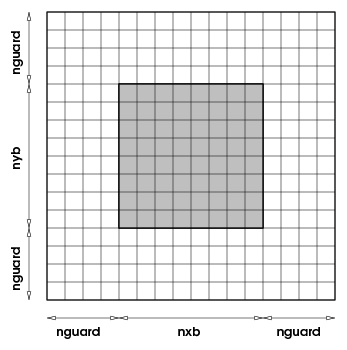
\includegraphics[width=3in]{Grid_single_block}}
\end{center}
\caption[A 2-D block with guard cells]{\label{Fig:single_block.eps} A
single 2-D block showing the
interior cells (shaded) and the perimeter of guard cells.}
\end{figure}

Any unit in the code can retrieve all or part of a block of data from
the \unit{Grid} unit along with the coordinates of corresponding
cells; it can then use this information for internal computations, and
finally return the modified data to the \unit{Grid} unit. The
\unit{Grid} unit also manages the parallelization of Flash-X. It
consists of a suite of subroutines which handle distribution of work
to processors and guard cell filling. When using an adaptive mesh, the
Grid unit is also responsible for refinement/derefinement and
conservation of flux across block boundaries. 

Flash-X can interchangeably use either
a \emterm{uniform} or \emterm{adaptive grid} for most
problems. Additionally, a new feature in \flashx is an option to
replicate the mesh; that is processors are assumed to be partitioned
into groups, each group gets a copy of the entire domain mesh. This
feature is useful when it is possible to decompose the computation
based upon certain compute intensive tasks that apply across the
domain. One such example is radiation transfer with multigroup flux
limited diffusion where each group needs an implicit solve. Here the 
state variable of the mesh are replicated on each group of processors,
while the groups are unique. Thus at the cost of some memory
redundancy, it becomes possible to compute a higher fidelity problem
(see \chpref{chp:RadTrans} for an example). 
Because of this feature, the parallel environment of the simulation is
now controlled by the Driver which differentiates between global
communicators and mesh communicators. The Grid unit queries the Driver
unit for mesh communicators. In all other respects this change is
transparent to the Grid unit. Mesh replication can be invoked through
the runtime parameter \rpi{Driver/meshCopyCount}

The uniform grid supported in Flash-X discretizes the physical domain by
placing grid points at regular intervals defined by the geometry of
the problem. The grid configuration remains unchanged throughout the
simulation, and exactly one block is mapped per processor.
An adaptive grid changes the discretization over the course of the
computation, and several blocks can be mapped to each computational
processor. Two AMR packages are currently supported in Flash-X for
providing adaptive grid capbility. The block-structured oct-tree based
AMR package, \Paramesh%\index{paramesh}
has been the work horse since
the beginning of the code. 

\begin {flashtip}
The following two commands will create the same (identical) application:
a simulation of a Sod shock tube in 3 dimensions with \Paramesh4
managing the grid.
\begin{codeseg}
./setup Sod -3d -auto

./setup Sod -3d -auto -unit=Grid/GridMain/paramesh/paramesh4/Paramesh4.0
\end{codeseg}
However, if the command is changed to
\begin{codeseg}
./setup Sod -3d -auto -unit=Grid/GridMain/UG
\end{codeseg}
the application is set up with a uniform grid instead.
Additionally, because two different grids types are supported in Flash-X, the user
must match up the correct \unit{IO} \childunit with the correct \unit{Grid} \childunit.
Please
see \chpref{Chp:IO} for more details.
Note that the \code{setup} script has capabilities to let the user set up
shortcuts, such as ``\code{+ugio}'', which makes sure that the appropriate
branch of \unit{IO} is included when the uniform grid is being used. Please see
\chpref{Sec:SetupShortcuts} for more information. Also see
% \tips{grid}{grid tips}
for shortcuts useful for the Grid unit.
\end{flashtip}

\section{\unit{GridMain} Data Structures}
The \unit{Grid} unit is the most extensive infrastructure unit in the
Flash-X code, and it owns data that most other units wish to fetch and
modify. Since the data layout in this unit has implications on the
manageability and performance of the code, we describe it in some
detail here. 

% First, unlike other units, \code{Grid} has two different
% \Fortran90 modules which contain the data variables.  In common with
% the structure of other units, there is
% \code{Grid_data.F90}. Additionally, there is the
% \code{physicaldata.F90} module, which contains the data types for all
% the physical-mesh based data. The split structure is necessary because
% Flash-X shares the \code{physicaldata.F90} module with \Paramesh.  
% To lessen confusion, the same name \code{physicaldata.F90} module is also defined in the \code{UG}
% (uniform grid) implementation.

Flash-X can be run with a grid discretization that assumes cell-centered data,
face-centered data, or a combination of the two. Paramesh and Uniform
Grid store physical data in multidimensional \Fortran90 arrays;
cell-centered variables in \code{unk}, short for ``unknowns'', and 
face-centered variables in arrays 
called \code{facevarx}, \code{facevary}, and \code{facevarz},
which contain the face-centered data along the
$x$, $y$, and $z$
dimensions, respectively. The cell-centered array \code{unk} is dimensioned as
\code{array(\code{NUNK_VARS},nxb,nyb,nzb,\metavar{blocks})},
 where \code{nxb}, \code{nyb}, \code{nzb} are the spatial dimensions
of a single block, and \metavar{blocks} is the number of blocks per
processor (\code{MAXBLOCKS} for \Paramesh and 1 for UG). The
face-centered arrays have one extra data point along the dimension
they are representing, for example \code{facevarx} is dimensioned as
\code{array(\code{NFACE_VARS},nxb+1,nyb,nzb,\metavar{blocks})}. 
 Some or all of the  actual values dimensioning these arrays are
determined at application setup time. The number of variables and the
value of \code{MAXBLOCKS} are always determined at setup time. The
spatial dimensions \code{nxb},\code{nyb},\code{nzb} can either be
fixed at setup time, or they may be determined at runtime. These two
modes are referred to as FIXEDBLOCKSIZE and
NONFIXEDBLOCKSIZE. 

All values determined at setup time are defined as constants in
a file \code{Flash.h} generated by the setup tool. This file contains
all application-specific global constants such as the number and
naming of physical variables, number and naming of fluxes and species,
\etc; it is described in detail in \chpref{Chp:Flash.h}.

For cell-centered variables, the \unit{Grid} unit
also stores a \emterm{variable type} that can be retrieved using 
the \api{Simulation/Simulation_getVarnameType} routine; see
\secref{Sec:ConfigFileSyntax} for the syntax and meaning
of the optional \code{TYPE} attribute that can be specified
as part of a \code{VARIABLE} definition read by the setup tool.

In addition to the primary physical variables, the \unit{Grid} unit has
another set of data structures for storing auxiliary fluid variables. 
This set of data structures provides a mechanism for storing such
variables whose spatial scope is the entire 
physical domain, but who do not need to maintain their guard cells
updated at all times. The data structures in this set include:
\code{SCRATCHCENTERVAR}, which has the same shape as the cell
centered variables data structure;  and \code{SCRATCHFACEXVAR},
\code{SCRATCHFACEYVAR} and \code{SCRATCHFACEZVAR}, which have
the same shape as the corresponding face centered variables
data structures. Early releases of Flash-X3 had \code{SCRATCHVAR},
dimensioned
\code{array(\code{NSCRATCH_GRID_VARS},nxb+1,nyb+1,nzb+1,blocks)}, as  
the only grid scope scratch data structure.  For reasons of backward
compatibility, and to maximize reusability of space, \code{SCRATCHVAR}
continues to exist as a supported data structure, though its use is
deprecated.  The
datastructures  
for face variables, though supported, are not used anywhere in the
released code base.  The unsplit MHD solver
\code{StaggeredMesh} discussed in \secref{Sec:usm_algorithm} gives an
example of the use of some of these data structures. It is important
to note that there is no guardcell filling for the scratch variables,
and the values in the scratch variables become invalid after a grid
refinement step. While users can define scratch variables to be
written to the plotfiles, they are not by default written to 
checkpoint files. The \unit{Grid} unit also stores the metadata
necessary for work distribution, load balancing, and other
housekeeping activities. These activities are further discussed in 
\secref{Sec:Grid UG} and \secref{Sec:Grid AMR}, which describe
individual implementations of the \unit{Grid} unit.


\section{Computational Domain}
\label{Sec:computational domain}
The size of the computational domain%\index{computational domain}
in
physical units is specified at runtime through the
(\rpi{Grid/xmin}, \rpi{Grid/xmax})%\index{grid!xmin/xmax@\code{xmin/xmax}},
(\rpi{Grid/ymin}, \rpi{Grid/ymax})%\index{grid!ymin/ymax@\code{ymin/ymax}}, and
(\rpi{Grid/zmin}, \rpi{Grid/zmax})%\index{grid!zmin/zmax@\code{zmin/zmax}}
runtime parameters.
When working with curvilinear coordinates (see
below in \secref{Sec:Grid geometry}), the extrema for angle
coordinates%\index{angular coordinates}
are specified in
degrees. Internally all angles are represented in radians, so angles
are converted to radians at \unit{Grid} initialization. 
\begin{flashtip}
The convention for specifying the ranges for angular coordinates
has changed from Flash-X2, which used units of $\pi$ instead of degrees
for angular coordinates.
\end{flashtip}

The physical domain is mapped into a computational domain at problem
initialization through routine \api{Grid/Grid_initDomain} in
\Paramesh and \api{Grid/Grid_init} in \code{UG}.When
using the uniform grid \code{UG}, the mapping is easy: one block is
created for each 
processor in the run, which can be sized either at build time or
runtime depending upon the mode of UG use. \footnote{Note that the
term processor, as used here and elsewhere in the 
documentation, does not necessarily correspond to a separate hardware
processor. It is also possible to have several logical ``processors''
mapped to the same hardware, which can be useful for debugging and
testing; this is a matter for the operating environment to regulate.} 
Further description can be found in \secref{Sec:Grid UG}.
When using the AMR grid \Paramesh, the mapping is non-trivial.
The adaptive mesh \code{gr\_createDomain} function creates an
initial mesh of \code{nblockx * nblocky * nblockz} top level blocks,
where \rpi{Grid/nblockx}, \rpi{Grid/nblocky}, and \rpi{Grid/nblockz}
are runtime parameters which default to 1.\footnote{The
\code{gr\_createDomain} function also can remove certain blocks of
this initial mesh, if this is requested by a non-default
\api{Simulation/Simulation_defineDomain} implementation.}
The resolution of the computational domain is usually very coarse and
unsuitable for computation after the initial mapping. The
\code{gr\_expandDomain} routine remedies the situation by applying the
refinement process to the initial domain until a satisfactory level of
resolution is reached everywhere in the domain. This method of mapping
the physical domain to computational domain is effective because the
resultant resolution in any section is related to the demands of the
initial conditions there. 

\begin{flashtip}
\flashx supported only an AMR grid with paramesh 2.  At initialization, it
created the coarsest level initial blocks
covering the domain using an algorithm called ``sequential'' divide domain.
A uniform grid of blocks on processor zero was created, and until the
first refinement, all blocks were on processor zero.  \flashx onwards
the paramesh based implementation of the Grid uses a ``parallel''
domain creation algorithm that attempts to create the initial domain
in blocks that are distributed amongst all processors according to the
same Morton ordering used by \Paramesh. 

First, the parallel algorithm computes a Morton number for each block
in the coarsest level uniform grid, producing a sorted list of Morton
numbers for all blocks to be created.  Each processor will create the
blocks from a section of this list, and each processor determines how
big its section will be.  After that, each processor loops over all
the blocks on the top level, computing Morton numbers for each,
finding them in the sorted list, and determining if this block is in
its own section.  If it is, the processor creates the block. Parallel
divide domain is especially useful in three-dimensional problems where
memory constraints can sometimes force the initial domain to be
unrealistically coarse with a sequential divide domain
algorithm. 
\end{flashtip} 


%------------------------------------------------------------------------
% Boundary conditions - text in separate file.
%------------------------------------------------------------------------
%using \input because of LaTeX Error: \include cannot be nested.
%------------------------------------------------------------------------
% Boundary conditions
%------------------------------------------------------------------------
\section{Boundary Conditions}
\label{Sec:BndryCond}

 Much of the \flashx code within the \unit{Grid} unit that deals with
implementing boundary conditions has been organized into a separate
\subunit, \unit{GridBoundaryConditions}.
Note that the following aspects are still handled elsewhere:
\begin{itemize}
\item Recognition of bounday condition  names as strings (in runtime parameters) 
and constants (in the source code); these are defined in 
\api{RuntimeParameters/RuntimeParameters_mapStrToInt} and in \code{constants.h},
respectively.
\item Handling of periodic boundary conditions; this is done within the underlying
\unit{GridMain} implementation. When using \Paramesh,
the subroutine \code{gr\_createDomain} is responsible for setting the
neighbors of top-level blocks (to either other top-level
blocks or to external boundary conditions) at initialization,
after \rpi{Grid/Nblockx} $\times$ \rpi{Grid/Nblocky} $\times$ \rpi{Grid/Nblockz}
root blocks have been created.
periodic (wrap-around) boundary conditions are initially configured in
this routine as well. If periodic boundary conditions are set in the
$x$-direction, for instance, the first blocks in the $x$-direction are
set to have as their left-most neighbor the blocks that are last in
the $x$-direction, and {\it vice versa}. Thus, when the guard cell
filling is performed, the periodic boundary conditions are
automatically maintained.
\item Handling of user-defined boundary conditions; this should be implemented
by code under the 
\newline
\unit{Simulation} directory.
\item
Low-level implementation and interfacing, such as are part of the \Paramesh code.
\item
Behavior of particles at a domain boundary. This is based on the boundary types
described below, but their handling is implemented
in \unit{GridParticles}.
\end{itemize}


Although the \unit{GridBoundaryConditions} \subunit is included in a
setup by default, it can be excluded (if no \code{Config} file
``\code{REQUIRES}'' it) by specifying
\code{-without-unit=Grid/GridBoundaryConditions}. This will generally
only make sense if all domain boundaries are to be treated as
periodic.  (All relevant runtime parameters
\rpi{Grid/xl_boundary_type} \etc need to be set to \code{"periodic"} in that
case.)

\subsection{Boundary Condition Types}
Boundary conditions %\index{boundary conditions}%\index{grid!boundary|see{boundary conditions}}
are determined by the physical problem.
%They are implemented
%by setting appropriate runtime parameters in flash.par, and filling the
%grid in \api{Simulation/Simulation_initBlock}.
Within Flash-X, the parallel structure of blocks means that each
processor works independently. If a block is on a physical boundary,
the  guard cells are filled by calculation
since there are no neighboring blocks from which to copy
values. Boundaries are selected by setting runtime parameters such as
\rpi{Grid/xl_boundary_type} (for the `left' $X$--boundary) to
one of the supported boundary types (\tblref{Tab:Boundaries}) in
\code{flash.par}. Even though the runtime parameters for specifying
boundary condition types are strings, the \unit{Grid} unit understands them as
defined integer constants defined in the file
\code{constants.h}, which contains all global constants for
the code. The translation from the string specified in
``flash.par'' to the constant understood by the \unit{Grid} unit is done by the
%% function \api{Simulation/Simulation_mapStrToInt}, which is generated by \code{setup}. %% -not so!
routine \api{RuntimeParameters/RuntimeParameters_mapStrToInt}.

\begin{table}[ht]
\label{Tab:Boundaries}
\begin{center}
\begin{tabular}{ll}
{\bf {\it ab}\_boundary\_type} & {\bf Description}\medskip\\
\hline
\code{periodic}     & Periodic (`wrap-around') \medskip\\
\code{reflect},\code{reflecting} & 
\begin{minipage}{0.6\textwidth}
Non-penetrating boundaries; plane symmetry,
the normal vector components change sign 
\end{minipage}
\medskip\\
\code{outflow}      & Zero-gradient boundary conditions; allows shocks
                     to leave the domain \medskip\\
\hline
\code{diode}        & 
\begin{minipage}{0.6\textwidth}
like outflow, but fluid velocities are never allowed to
                      let matter flow into the domain: normal velocity components are
		      forced to zero in guard cells if necessary
\end{minipage}
\medskip\\
\hline
\code{axisymmetric} & 
\begin{minipage}{0.6\textwidth}
like \code{reflect}, but both normal and toroidal vector components change sign.
Typically used with cylindrical geometry (R-Z) for the Z symmetry axis.
\end{minipage}
\medskip\\
\code{eqtsymmetric} & 
\begin{minipage}{0.6\textwidth}
like reflect for velocities but the magnetic field components, poloidal and toroidal,
change sign. The sign of the normal magnetic field component remains the same.
Typically used with cylindrical geometry (R-Z) for the R axis to emulate equatorial
symmetry.
\end{minipage}
\medskip\\
\hline
\code{hydrostatic-f2}  & Hydrostatic boundary handling as in \flashx. See remark in text. \medskip\\
\hline
\begin{minipage}{0.25\textwidth}
\code{hydrostatic-f2+nvrefl},
\code{hydrostatic-f2+nvout},
\code{hydrostatic-f2+nvdiode}
\end{minipage}
&
\begin{minipage}{0.6\textwidth}
Variants of \code{hydrostatic-f2}, where the \textbf{n}ormal \textbf{v}elocity
is handled specially in various ways, analogous to
\code{reflect}, \code{outflow}, and \code{diode} boundary conditions, respectively. See remark in text.
\end{minipage}
\medskip\\
\hline
\begin{minipage}{0.2\textwidth}
\code{user-defined}
 or \code{user}
\end{minipage}
&
\begin{minipage}{0.6\textwidth}
The user must implement the desired boundary behavior; see text.
\end{minipage}
\medskip\\
\hline
\end{tabular}
\caption{  Hydrodynamical boundary conditions supported by Flash-X. Boundary type {\it ab} may be
replaced with $a$=\{x,y,z\} for direction and $b$=\{l,r\} for left/right edge.
All boundary types listed except the last (\code{user}) have an implementation in \unit{GridBoundaryConditions}.}
\end{center}
\end{table}

To use any of the \code{hydrostatic-f2*} boundary conditions, the setup must
include \code{Grid/GridBoundary\-Conditions/\-Flash2HSE}.  This must
usually be explicitly requested, for example with a line
\begin{codeseg}
REQUIRES Grid/GridBoundaryConditions/Flash2HSE
\end{codeseg}
in the simulation directory's \code{Config} file.

% \begin{comment}
% \code{hydrostatic}  & Supports the fluid `above' against gravity \\
% \code{diode}        & like outflow, but fluid velocities are never allowed to
% The user must override the default
% \api{Grid/Grid_applyBCEdge} with an implementation
% that adds the desired boundary behavior.
% \end {comment}


Note that the \rpi{Gravity/grav_boundary_type} runtime parameter is 
used by some implementations of the \unit{Gravity} unit
to define the type of boundary for solving a self-gravity (Poisson) problem;
see \api{physics/Gravity/Gravity_init}. This runtime parameter is
separate from the {\bf {\it ab}\_boundary\_type} ones interpreted
by \unit{GridBoundaryConditions}, and its recognized values are
not the same (although there is some overlap).


\begin{table}[ht]
\begin{center}
\begin{tabular}{lll}
{\bf {\it ab}\_boundary\_type} & {\bf Constant}& {\bf Remark}\\
\hline
\code{isolated}        & --- & used by Gravity only for \rpi{Gravity/grav_boundary_type} \\
---                    & \code{DIRICHLET} & used for multigrid solver \\
---                    & \code{GRIDBC\_MG\_EXTRAPOLATE} & for use by multigrid solver\\
---                    & \code{PNEUMANN} & (for use by multigrid solver) \\
\hline
\code{hydrostatic}  & \code{HYDROSTATIC} &  Hydrostatic, other implementation than \flashx \\
\hline
\code{hydrostatic+nvrefl}& \code{HYDROSTATIC\_NVREFL} &  Hydrostatic variant, other impl.~ than \flashx \\
\code{hydrostatic+nvout}& \code{HYDROSTATIC\_NVOUT} &  Hydrostatic variant, other impl.~ than \flashx \\
\code{hydrostatic+nvdiode}& \code{HYDROSTATIC\_NVDIODE} &  Hydrostatic variant, other impl.~ than \flashx \\
\hline
\hline
\end{tabular}
\caption{Additional boundary condition types recognized by Flash-X. Boundary type {\it ab} may be
replaced with a=\{x,y,z\} for direction and b=\{l,r\} for left/right edge.
These boundary types are either reserved for implementation by users and/or future
Flash-X versions for a 
specific purpose (as indicate by the remarks), or are for special uses
within the \unit{Grid} unit.}
\label{Tab:RecognizedBoundaries}
\end{center}
\end{table}




\subsection{Boundary Conditions at Obstacles}

The initial coarse grid of root blocks can be modified by removing certain blocks.
This is done by providing a non-trivial implementation of
\api{Simulation/Simulation_defineDomain}. Effectively this creates
additional domain boundaries at the interface between blocks removed
and regions still included. All boundary conditions other than
\code{periodic} are possible at these additional boundaries, and
are handled there in the same way as on external domain boundaries.
This feature is only available with \Paramesh.
See the documentation and example in \api{Simulation/Simulation_defineDomain}
for more details and some caveats.

\subsection{Implementing Boundary Conditions}

Users may need to implement boundary conditions
beyond those provided with \flashx, and the \unit{Grid\-Boundary\-Conditions} \subunit
provides several ways to achieve this.
Users can provide an implementation for the \code{user} boundary type;
or can provide or override an implementation for one of the other
recognized types.

The simple boundary condition types \code{reflect},
\code{outflow}, \code{diode} are implemented in the
\newline
\api{Grid/Grid_bcApply\-To\-Region}\code{.F90} file in
\code{Grid/GridBoundaryConditions}.  A users can
add or modify the handling of some boundary condition
types in a version of this file in the simulation directory,
which overrides the regular version.  There is, however, also
the interface \api{Grid/Grid_bcApplyToRegionSpecialized}
which by default is only provided as a stub and is
explicitly intended to be implemented by users.
\newline
A \api{Grid/Grid_bcApplyToRegionSpecialized} implementation
gets called before \api{Grid/Grid_bcApplyToRegion}
and can decide to either handle a specific combination
of boundary condition type, direction, grid data structure, \etc,
or leave it to \api{Grid/Grid_bcApplyToRegion}.
These calls operate on a region of one block's cells at a time.
Flash-X will pass additional information beyond that needed
for handling simple boundary conditions to 
\api{Grid/Grid_bcApplyToRegionSpecialized}, in particular
a block handle through which an implementation can
retrieve coordinate information and access
other information associated with a block and its cells.

The \unit{GridBoundaryConditions} \subunit also provides
a simpler kind of interface if one includes 
\code{Grid/\-GridBoundaryConditions/OneRow} in the setup.
When using this style of interface, users can implement
guard cell filling one row at a time. Flash-X passes
to the implementation one row of cells at a time,
some of which are interior cells while the others
represent guard cells outside the boundary that are
to be modified in the call.
A row here means a contiguous set of cells along a line perpendicular
to the boundary surface.
There are two versions of this interface:
\api{Grid/Grid_applyBCEdge} is given only one fluid
variable at a time, but can also handle data structures
other than \code{unk}; whereas \api{Grid/Grid_applyBCEdgeAllUnkVars}
handles all variables of \code{unk} along a row in one call.
Cell coordinate information is included in the call arguments.
Flash-X invokes these functions through an implementation
of \api{Grid/Grid_bcApplyToRegionSpecialized} in
\code{Grid/GridBoundaryConditions/OneRow} which acts as a wrapper.
\code{GridBoundaryConditions/OneRow} also provides a default
implementation of \api{Grid/Grid_applyBCEdge} (which implements
the simple boundary conditions) and \api{Grid/Grid_applyBCEdgeAllUnkVars}
(which calls \code{Grid\_applyBCEdge}) each.
Another implementation of \api{Grid/Grid_applyBCEdgeAllUnkVars}
can be found in
\code{GridBoundaryConditions/OneRow/Flash2HSE},
this one calls \code{Grid\_applyBCEdge} or, for \flashx-type
hydrostatic boundaries, the code for handling them.
These can be used as templates for overriding implementations
under \code{Simulation}.
It is not recommended to try to mix both \code{Grid\_bcApplyToRegion*}-style
and \code{Grid\_applyBCEdge*}-style overriding implementations in
a simulation directory, since this could become confusing.


Note that in all of these cases, \ie, whether boundary guard
cell filling for a boundary type is implemented in
\api{Grid/Grid_bcApplyToRegion},
\api{Grid/Grid_bcApplyToRegionSpecialized},
\api{Grid/Grid_applyBCEdge}, or
\newline
\api{Grid/Grid_applyBCEdge\-AllUnkVars}, the implementation
does not fill guard cells in permanent data storage (the
\code{unk} array and similar data structures) directly,
but operates on buffers. \flashx fills some parts of the buffers
with current values for interior cells before the
call, and copies updated guardcell data from some (other) parts
of the buffers back into \code{unk} (or similar) storage
after the handling routine returns.

All calls to handlers for boundary conditions are for one face in a given
dimension at a time. Thus for each of the
\code{IAXIS}, \code{JAXIS}, and \code{KAXIS} dimensions there can be up to
two series of calls, once for
the left, \ie, ``\code{LOW},'' and once for the right, \ie,
``\code{HIGH},'' face.  \Paramesh4 makes additional calls
for filling guard cells in edge and corner regions of blocks,
these calls result in additional \code{Grid\_bcApplyToRegion*}\ invocations
for those cells that lie in diagonal directions from the block interior.

The boundary condition handling interfaces described so far can
be implemented (and will be used!) independent of the \unit{Grid}
implementation chosen. At a lower level, the various implementations
of \unit{GridMain} have different ways of requesting that
boundary guard cells be filled. The \unit{GridBoundaryConditions} \subunit
collaborates with \unit{GridMain} implementations to provide to user code
uniform interfaces that are agnostic of lower-level details.
However, it is also possible --- but not recommended --- for users to
replace a routine that is located
deeper in the \unit{Grid} unit. For \Paramesh4, the most relevant
routine is \code{amr\_1blk\_bcset.F90}, for \Paramesh2 it is
\code{tot\_bnd.F90}, and for uniform grid \code{UG} it is
\code{gr\_bcApplyToAllBlks.F90}.

\subsubsection{Additional Concerns with \Paramesh4}
Boundary condition handling has become significantly more complex in \flashx.
In part this is so because \Paramesh4 imposes requirements on
guard cell filling code that do not exist in the other \code{GridMain}
implementations:
\begin{enumerate}
\item In other \code{Grid} implementations, filling of domain boundary guard cells
is under control of the ``user'' (in this context, the user of the grid implementation,
\ie, Flash-X): These cells can be filled for all blocks at a time that is predictable to the user
code, as a standard part of handling \api{Grid/Grid_fillGuardCells}, only.
With \Paramesh4, the user-provided \code{amr\_1blk\_bcset} routine can be called
from within the depths of \Paramesh on individual blocks (and cell regions, see below)
during guard cell filling and at other times when the user has called a \Paramesh
routine. It is not easy to predict when and in which sequence this will happen.
\item \Paramesh4 does not want all boundary guard cells filled in one call,
but requests individual regions in various calls.
\item \Paramesh4 does not let the user routine \code{amr\_1blk\_bcset} operate on 
permanent storage (\code{unk} \etc) directly, but on (regions of) one-block
buffers.
\item \Paramesh4 occasionally invokes \code{amr\_1blk\_bcset} to operate on 
regions of a block that belongs to a remote processor (and for which
data has been cached locally). Such block data is not associated with
a valid local \code{blockID}, making it more complicated for user
code to retrieve metadata that may be needed to implement the
desired boundary handling.
\end{enumerate}

Some consequences of this for \flashx users:
\begin{itemize}
\item
User code that implements boundary conditions for the grid inherits
the requirement that it must be ready to be called at various times
(when certain \unit{Grid} routines are called).
\item
User code that implements boundary conditions for the grid inherits
the requirement that it must operate on a region of the cells of
a block, where the region is specified by the caller.
\item
Such user code must not assume that it operates on permanent data (in \code{unk} \etc).
Rather, it must be prepared to fill guardcells for a block-shaped buffer
that may or may not end up being copied back to permanent storage.

User code also is not allowed to make certain \Paramesh4 calls while
a call to  \code{amr\_1blk\_bcset} is active, namely those that
would modify the same one-block buffers that the current call
is working on.
\item
The user code must not assume that the block data it is acting on belongs to
a local block. The data may not have a valid \code{blockID}.
The code will be passed a ``block hande'' which can be used
in some ways, but not all, like a valid \code{blockID}.
%This last point may be most onerous.
\end{itemize}

 

%------------------------------------------------------------------------
% UG
%------------------------------------------------------------------------
\section{Uniform Grid} 
\label{Sec:Grid UG} 

The Uniform Grid has the same resolution in all the blocks throughout
the domain, and each processor has exactly one block.  The uniform
grid can operate in either of two modes: fixed block size
(FIXEDBLOCKSIZE) mode, and non-fixed block size (NONFIXEDBLOCKSIZE)
mode. The default fixed block size grid is statically defined at
compile time and can therefore take advantage of compile-time
optimizations. The non-fixed block size version uses dynamic memory
allocation of grid variables. 

\subsection{FIXEDBLOCKSIZE Mode} 
\code{FIXEDBLOCKSIZE}%\index{FIXEDBLOCKSIZE mode}
mode, also called
static mode, is the default for the uniform grid. In this mode, the
block size is specified at compile time as
\code{NXB}$\times$\code{NYB}$\times$\code{NZB}. These variables
default to $8$ if the dimension is defined and $1$ otherwise -- \eg
for a two-dimensional simulation, the defaults are \code{NXB}$=8$,
\code{NYB}$=8$, \code{NZb}$=1$. To change the static dimensions,
specify the desired values on the command line of the \code{setup}
script; for example 
\begin{codeseg} 
./setup Sod -auto -3d -nxb=12 -nyb=12 -nzb=4 +ug
\end{codeseg} 
The distribution of processors along the three dimensions is given at 
run time as $iprocs\times jprocs\times kprocs$ with the constraint 
that this product must be equal to the number of processors that the 
simulation is using. The global domain size in terms of number of grid
points is $\code{NXB}*iprocs \times \code{NYB}*jprocs \times 
\code{NZB}*kprocs$.  For example, if $iprocs=jprocs=4$ and $kprocs=1$,
the execution command should specify $np=16$ processors.
\begin{codeseg} 
mpirun -np 16 flash3 
\end{codeseg} 
When working in static mode, the simulation is constrained to run on 
the same number of processors when restarting, since any different 
configuration of processors would change the domain size. 

At Grid initialization time, the domain is created and the 
communication machinery is also generated. This initialization 
includes MPI communicators and datatypes for directional guardcell 
exchanges. If we view processors as arranged in a three-dimensional 
processor grid, then a row of processors along each dimension becomes 
a part of the same communicator. We also define MPI datatypes for each
of these communicators, which describe the layout of the block on the
processor to MPI. The communicators and datatypes, once generated, 
persist for the entire run of the application. Thus the 
\code{MPI\_SEND/RECV} function with specific communicator and its 
corresponding datatype is able to carry out all data exchange for 
guardcell fill in the selected direction in a single step. 

Since all blocks exist at the same resolution in the Uniform Grid, 
there is no need for interpolation%\index{grid!interpolation}
while
filling the guardcells. Simple exchange of correct data between
processors, and the application of boundary conditions where needed is
sufficient. The guard cells along the face of a block are filled with
the layers of the interior cells of the block on the neighboring
processor if that face is shared with another block, or calculated
based upon the boundary conditions if the face is on the physical
domain boundary. Also, because there are no jumps in refinement in the
Uniform Grid, the flux conservation step across processor boundaries
is unnecessary. For correct functioning of the Uniform Grid in Flash-X, 
this conservation step should be explicitly turned off with  a runtime
parameter \rpi{Grid/flux_correct} which controls whether or not to run
the flux conservation step in the PPM Hydrodynamics
implementation. AMR sets it by default to true, while UG sets
it to false. Users should exercise care if they wish to override the 
defaults via their ``\code{flash.par}'' file. 

\subsection{NONFIXEDBLOCKSIZE  mode}\label{Sec:NONFIXEDBLOCKSIZE}%\index{NONFIXEDBLOCKSIZE mode}
Up ot version 2, Flash-X always ran in a mode where all blocks have
exactly the same number of grid points in exactly the same shape, and these
were fixed at compile time. Flash-X was limited to use the fixed block
size mode described above. With \flashx this constraint was eliminated
through an option at setup time. The two main reasons for this
development were: one, to allow a uniform grid based simulation to be
able to restart with different number of processors, and two, to open up
the possibility of using other AMR packages with
Flash-X. Patch-based packages typically have different-sized
block configurations at different times. This mode,
called the ``NONFIXEDBLOCKSIZE'' mode, can currently be selected for
use with Uniform Grid. To run an
application in ``NONFIXEDBLOCKSIZE'' mode%\index{NONFIXEDBLOCKSIZE mode},
the ``\code{-nofbs}'' option must be used when invoking the setup
tool; see \chpref{Chp:The Flash-X configuration script} for more information.
For example:
\begin{codeseg}
./setup Sod -3d -auto -nofbs
\end{codeseg}
Note that \code{NONFIXEDBLOCKSIZE} mode requires the use of its own IO implementation, 
and a convenient shortcut has been provided to ensure that this mode is used as 
in the example below:
\begin{codeseg}
./setup Sod -3d -auto +nofbs
\end{codeseg}

In this mode, the blocksize in UG is determined at execution
from runtime parameters \rpi{Grid/iGridSize},
\rpi{Grid/jGridSize} and
\rpi{Grid/kGridSize}. These parameters specify the global
number of grid points in the computational domain along each
dimension. The blocksize then is
$(iGridSize/iprocs)\times(jGridSize/jprocs)\times(kGridSize/kprocs)$.

Unlike \code{FIXEDBLOCKSIZE} mode, where memory %\index{memory}
is allocated
at compile time, in the \code{NONFIXEDBLOCKSIZE}
mode%\index{NONFIXEDBLOCKSIZE mode}  all memory%\index{memory}
allocation is dynamic.  The global data structures are allocated when
the simulation initializes and deallocated when the simulation
finalizes, whereas the local scratch space is allocated and
deallocated every time a unit is invoked in the simulation. Clearly
there is a trade-off between flexibility and performance as the
\code{NONFIXEDBLOCKSIZE} mode typically runs about 10-15\% slower.  We
support both to give choice to the users. The amount of memory
consumed by the Grid data structure of the Uniform Grid is
$\code{nvar} \times (2*\code{nguard}+\code{nxb}) \times
(2*\code{nguard}+\code{nyb})\times(2*\code{nguard}+\code{nzb})$
irrespective of the mode.  Note that this is not the total amount of
memory used by the code, since fluxes, temporary variables, coordinate
information and scratch space also consume a large amount of memory.

The example shown below gives two possible ways to define parameters
in \code{flash.par} for a 3d problem of global domain size $64 \times
64 \times 64$, being run on 8 processors.
\begin{codeseg}
iprocs = 2
jprocs = 2
kprocs = 2
iGridSize = 64
jGridSize = 64
kGridSize = 64
\end{codeseg}
This specification will result in each processor getting a block of
size $32 \times 32 \times 32$. Now consider the following
specification for the number of processors along each dimension,
keeping the global domain size the same.
\begin{codeseg}
iprocs = 4
jprocs = 2
kprocs = 1
\end{codeseg}
In this case, each processor will now have blocks of size $ 16 \times 32 \times 64$.



%------------------------------------------------------------------------
% AMR
%------------------------------------------------------------------------
\section{Adaptive Mesh Refinement (AMR) Grid with Paramesh}
\label{Sec:Grid AMR}


The default package in Flash-X is
\Paramesh%\index{PARAMESH}%\index{adaptive mesh}
(MacNeice {\it et al.}\ 1999) for implementing the adaptive mesh
refinement (AMR) grid. \Paramesh uses a block-structured adaptive mesh
refinement scheme similar to others in the literature (\eg, Parashar
1999; Berger \& Oliger 1984; Berger \& Colella 1989; DeZeeuw \& Powell
1993).  It also shares ideas with schemes which refine on an
individual cell basis (Khokhlov 1997).  In block-structured AMR, the
fundamental data structure is a block of cells arranged in a logically
Cartesian fashion. ``Logically Cartesian'' implies that each
cell can be specified using a block identifier
(processor number and local block number) and a coordinate triple
$(i,j,k)$, where $i=1\ldots\code{nxb}$, $j=1\ldots\code{nyb}$, and
$k=1\ldots\code{nzb}$ refer to the $x$-, $y$-, and $z$-directions,
respectively.   It does not require a physically rectangular coordinate system;
for example a spherical grid can be indexed in this same manner.
%Note, however, that this release of Flash-X3 only supports logically- and
%physically-Cartesian problems.

The complete computational grid consists of a collection
of blocks with different physical cell sizes, which are related to
each other in a hierarchical fashion using a tree data structure. The
blocks at the root of the tree have the largest cells, while their
children have smaller cells and are said to be refined. Three rules
govern the establishment of refined child blocks in \Paramesh. First, a
refined child block must be one-half as large as its parent block in
each spatial dimension. Second, a block's children must be nested;
\ie, the child blocks must fit within their parent block and cannot
overlap one another, and the complete set of children of a block must
fill its volume. Thus, in $d$ dimensions a given block has either zero
or $2^d$ children.  Third, blocks which share a common border may not
differ from each other by more than one level of refinement.

A simple two-dimensional domain is shown in
\figref{Fig:block_structure.eps}, illustrating the rules above. Each
block contains $\code{nxb}\times\code{nyb}\times\code{nzb}$ interior
cells and a set of guard cells. The guard cells contain boundary
information needed to update the interior cells. These can be obtained
from physically neighboring blocks, externally specified boundary
conditions, or both.
\begin{figure}
\begin{center}
{\leavevmode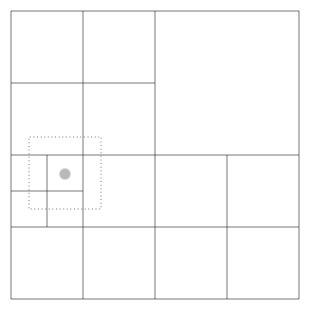
\includegraphics[width=3in]{Grid_block_structure}}
\end{center}
\caption{\label{Fig:block_structure.eps} A simple computational domain showing
varying levels of refinement in a total of 16 blocks.  The dotted lines outline the
guard cells for the block marked with a circle.}
\end{figure}
The number of guard cells needed depends upon the interpolation schemes
and the differencing stencils used by the various physics units (usually
hydrodynamics). For the explicit PPM algorithm distributed with Flash-X,
four guard cells are needed in each direction, as illustrated in
\figref{Fig:single_block.eps}. The blocksize while using the adaptive
grid is fixed at compile time, resulting in static
memory%\index{memory}
allocation.  The total number of blocks a
processor can manage is determined by
\code{MAXBLOCKS}%\index{MAXBLOCKS@\code{MAXBLOCKS}},
which can be
overridden at setup time with the \code{setup \ldots -maxblocks=\#}
argument. The amount of memory consumed by the Grid data structure of
code when running with \Paramesh is $\code{NUNK\_VARS} \times
(2*\code{nguard}+\code{nxb}) \times
(2*\code{nguard}+\code{nyb}) \times
(2*\code{nguard}+\code{nzb}) \times \code{MAXBLOCKS}$. \Paramesh
also needs memory to store its tree data structure for adaptive mesh
management, over and above what is already mentioned with Uniform
Grid. As the levels of refinement increase, the size of the tree also
grows.

%%%%%%%%%%%%%%  next 2 paras anticipate INTERP subsection %%%%%%%%%%%%
\Paramesh handles the filling of guard cells with information from
other blocks or, at the boundaries of the physical domain, from an
external boundary routine (see \secref{Sec:BndryCond}).
If a block's neighbor exists and has the same level of refinement,
\Paramesh fills the corresponding guard cells using a direct copy from
the neighbor's interior cells. If the neighbor has a different level
of refinement, the data from the neighbor's cells must be adjusted by
either interpolation%\index{grid!interpolation}
(to a finer level of
resolution) or averaging (to a coarser level)%\index{grid!data averaging}
---see \secref{Sec:gridinterp} below for more information.
If the block and its neighbor are stored in the memory of
different processors, \Paramesh handles the appropriate parallel
communications (blocks are never split between processors).
The filling of guard cells is a global operation that is
triggered by calling \api{Grid/Grid_fillGuardCells}.

Grid Interpolation%\index{grid!interpolation}
is also used when filling
the blocks of children newly created in the course of automatic
refinement. This happens during \api{Grid/Grid_updateRefinement}
processing. Averaging%\index{grid!data averaging}
is also used 
to regularly update the solution data in at least one level of parent
blocks in the oct-tree. This ensures that after leaf nodes are
removed during automatic refinement processing (in regions of the
domain where the mesh is becoming coarser), the new leaf nodes
automatically have valid data.
This averaging happens as an initial step in
\api{Grid/Grid_fillGuardCells} processing.

\Paramesh also enforces flux conservation %\index{flux
                                %conservation}\label{Sec:PARAMESH flux
                                %conservation}
at jumps
in refinement, as described by Berger and Colella (1989).  At jumps
in refinement, the fluxes of mass, momentum, energy (total and
internal), and species density in the fine cells across boundary
cell faces are summed and passed to their parent.  The parent's
neighboring cell will be at the same level of refinement as the summed
flux cell because \Paramesh limits the jumps in refinement to one level
between 
blocks.  The flux in the parent that was computed by the more
accurate fine cells is taken as the correct flux through the
interface and is passed to the corresponding coarse face on the
neighboring block (see \figref{Fig:flux_conservation_fig}). The
summing allows a geometrical weighting to be implemented for
non-Cartesian geometries, which ensures that the proper volume-corrected
flux is computed.

\begin{figure}
\begin{center}
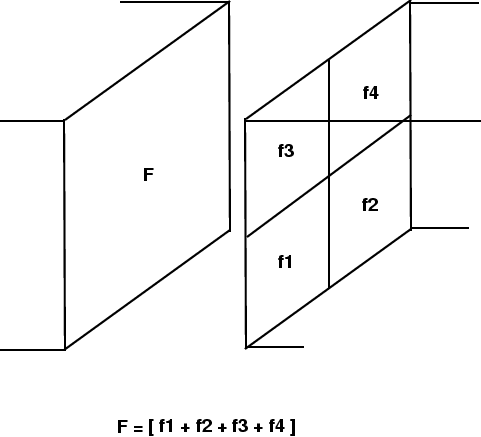
\includegraphics[height=2.5in]{Grid_flux_cons}
\caption{\label{Fig:flux_conservation_fig}
        Flux conservation at a jump in refinement.  The fluxes in the fine
        cells are added and replace the coarse cell flux (F).}
\end{center}
\end{figure}

\subsection{Additional Data Structures}
\label{Sec:amr data struct}
\Paramesh maintains much additional information about the mesh.
In particular, oct-tree related information is kept 
in various arrays which are declared in a
\Fortran90 module called ``\code{tree}''.
It includes
% information about a block's Morton number,
the physical coordinate of a block's center, its physical size,
level of refinement, and
much more. These data structures also acts as temporary storage while
updating refinement in the grid and moving the blocks.
This metadata should in general not be accessed directly by application code.
The \unit{Grid} API contains subroutines for accessing the most important
pars of this metadata on a block by block basis, like
\api{Grid/Grid_getBlkBoundBox},
\api{Grid/Grid_getBlkCenterCoords},
\api{Grid/Grid_getBlkPhysicalSize},
\api{Grid/Grid_getBlkRefineLevel}, and
\api{Grid/Grid_getBlkType}.

Flash-X has its
own \code{oneBlock} data structure that stores block specific
information. This data structure keeps the physical coordinates of
each cell in the block. For each dimension, the coordinates are stored
for the \code{LEFT_EDGE}, the \code{RIGHT_EDGE} and the center of the cell. The
coordinates are determined from ``{\it cornerID}'' which is also a part of
this data structure.

The concept of \code{cornerID} was introduced in \flashx; it serves three
purposes. First, it creates a unique global identity for every cell
that can come into existence at any time in the course of the
simulation.   Second, it can prevent machine precision error from
creeping into the spatial coordinates calculation. Finally, it can
help pinpoint the location of a block within the oct-tree of
\Paramesh. Another useful integer variable is the concept of a {\it
stride}. A stride indicates the spacing factor between one cell and
the cell directly to its right when calculating the cornerID.   At the
maximum refinement level, the stride is $1$, at the next higher level
it is $2$, and so on. Two consecutive cells at refinement level $n$
are numbered with a stride of $2^{lrefine\_max-n}$ where $1 \le n \le
lrefine\_max$.

The routine \api{Grid/Grid_getBlkCornerID} provides a convenient way
for the user to retrieve the location of a block or cell.  A usage
example is provided in the  documentation for that routine.
The user should retrieve accurate physical and grid coordinates by
calling the routines \api{Grid/Grid_getBlkCornerID},
\api{Grid/Grid_getCellCoords}, \api{Grid/Grid_getBlkCenterCoords} and
\api{Grid/Grid_getBlkPhysicalSize}, instead of calculating their own
from local block information, since they take advantage of the
\code{cornerID} scheme, and therefore avoid the possibility of
introducing machine precision induced numerical drift in the calculations.


%------------------------------------------------------------------------
% INTERPOLATION
%------------------------------------------------------------------------
\subsection[Grid Interpolation]{Grid Interpolation (and Averaging)}
\label{Sec:gridinterp}
The adaptive grid requires data \emterm{interpolation} or
\emterm{averaging} when the refinement level 
(\ie, mesh resolution) changes in space or in time.
\footnote{Particles and Physics units may make additional use of
interpolation as part 
of their function, and the algorithms may or may not be different.
This subsection only discusses interpolation automatically performed by the
\unit{Grid} unit on the fluid variables in a way that should be transparent to other units.}
If during guardcell filling a block's neighbor has a coarser level of
refinement, the neighbor's cells are used to \emterm{interpolate}
guard cell values to the cells of the finer block. 
Interpolation%\index{grid!interpolation}
is also used when filling the blocks
of children newly created in the course of automatic refinement.
Data \emterm{averaging} is used to adapt data in the opposite direction, \ie,
from fine to coarse.

In the AMR context, the term \emterm{prolongation}%\index{grid!prolongation}
is used to refer to data interpolation
(because it is used when the tree of blocks grows longer).
Similarly, the term \emterm{restriction}%\index{grid!restriction}
is used to refer to fine-to-coarse data averaging.

The algorithm used for restriction is straightforward (equal-weight)
averaging in Cartesian coordinates, but has to
take cell volume factors into account for curvilinear coordinates;
see \secref{Sec:Non-Cart Prol/Rest}.


\Paramesh supports various interpolation%\index{grid!interpolation}
schemes, to which user-specified interpolation schemes can be added.
\flashx currently allows to choose between two interpolation schemes:
\begin{enumerate}
\item monotonic
\item native
\end{enumerate}
The choice is made at \code{setup} time, see \secref{Sec:ListSetupArgs}.


%for guard cell filling at jumps at refinement

The versions of \Paramesh supplied with \flashx supply their own
default interpolation scheme, which is used when \flashx is
configured with the \code{-gridinterpolation=native} \code{setup}
option (see \secref{Sec:ListSetupArgs}). The default schemes are only
appropriate for Cartesian coordinates. If \flashx is configured
with curvilinear support, an alternative scheme (appropriate for all
supported geometries) is compiled in. This so-called
``\emterm{monotonic}'' interpolation attempts to ensure that
interpolation does not introduce small-scale non-monotonicity in the
data. The order of ``monotonic'' interpolation can be chosen with the
\rpi{Grid/interpol_order}%\index{grid!interpolation!order}
runtime
parameter. See \secref{Sec:Non-Cart Prol/Rest} for some more details
on prolongation for curvilinear coordinates.  At setup time, monotonic
interpolation is the default interpolation used.

%\begin{flashtip}
% an entire page is not a ``tip''
\subsubsection{Interpolation for mass-specific solution variables}
\label{Sec:InterpMassSpecific}
To accurately preserve the total amount of conserved quantities,
the interpolation routines have to be applied to solution data in
\emterm{conserved}, \ie, volume-specific, form. However, many variables
are usually stored in the \code{unk} array in mass-specific form,
\eg, specific internal and total energies, velocities, and mass
fractions. See \secref{Sec:ConfigFileSyntax} for how to use
the optional \code{TYPE} attribute in a \code{Config} file's
\code{VARIABLE} definitions to inform the \unit{Grid} unit
which variables are considered mass-specific.

\flashx provides three ways to deal with this:
\begin{enumerate}
\item Do nothing---\ie, assume that ignoring the difference between
mass-specific and conserved form is a reasonable approximation.
Depending on the smoothness of solutions in regions where refinement,
derefinement, and jumps in refinement level occur, this assumption may
be acceptable.
This behavior can be forced 
by setting the
%\newline
\rpi{Grid/convertToConsvdInMeshInterp} runtime parameter to \code{.false.}

\item Convert mass-specific variables to conserved form
\emph{in all blocks throughout the physical domain}
before invoking a \unit{Grid} function that may
result in some data interpolation or restriction (refinement,
derefinement, guardcell filling); and convert back after these
functions return. Conversion is done by cell-by-cell multiplication
with the density (\ie, the value of the ``\code{dens}'' variable, which should be declared as
\begin{codeseg}
VARIABLE dens TYPE: PER_VOLUME
\end{codeseg}
in a \code{Config} file).

This behavior is available in both \Paramesh2  and \Paramesh4.
It is enabled by setting the 
\newline 
\rpi{Grid/convertToConsvdForMeshCalls}
runtime parameter and corresponds roughly to \flashx with
\newline
\code{conserved_var} enabled.

\item Convert mass-specific variables to conserved form
only where and when necessary, from the \code{Grid} user's
point of view \emph{as part of data interpolation}.
Again, conversion is done by cell-by-cell multiplication
with the value of density.
In the actual implementation of this approach, the
conversion and back-conversion operations are
closely bracketing the interpolation (or restriction) calls.
The implementation avoids spurious back-and-forth
conversions (\ie, repeated successive
multiplications and divisions of data by the density)
in blocks that should not be modified by interpolation or restriction.

This behavior is available only for \Paramesh4.
As of \flashx, this is the default behavior whenever available.
It can be enabled explicitly 
(only necessary in setups that change the default) by setting the
\newline
\rpi{Grid/convertToConsvdInMeshInterp} runtime parameter.

\end{enumerate}
%\end{flashtip}




\subsection{Refinement}
\label{Sec: refinement}
%------------------------------------------------------------------------
% Refinement criteria
%------------------------------------------------------------------------
\subsubsection{Refinement Criteria}
The refinement criterion used by \Paramesh is adapted from L\"ohner (1987).
L\"ohner's error estimator was originally developed for finite element
applications and has the advantage that it uses a mostly  local
calculation. Furthermore, the estimator is dimensionless and can be
applied with complete generality to any of the field variables of the
simulation or any combination of them.

\begin{flashtip}
\flashx does not define any refinement variables by default.
Therefore simulations using AMR have to make the appropriate runtime parameter
definitions in \code{flash.par}, or in the simulation's \code{Config} file.
If this is not done, the program generates a warning at startup, and no
automatic refinement will be performed. The mistake of
not specifying refinement variables
is thus easily detected.
To define a refinement variable, use \rpi{Grid/refine_var_\#}
(where \code{\#} stands for a number from 1 to 4)
in the \code{flash.par} file.
\end{flashtip}

L\"ohner's estimator is a modified second
derivative, normalized by the average of the gradient over one
computational cell. In one dimension on a uniform mesh, it is given by

\begin{equation}
E_{i} = { \frac{ \mid u_{i+1} - 2u_{i} + u_{i-1} \mid}
%          \over
         { \mid u_{i+1} - u_{i} \mid + \mid u_{i} - u_{i-1} \mid +
              \epsilon [ \mid u_{i+1} \mid + 2 \mid  u_{i} \mid +
                          \mid u_{i-1} \mid ] }\ } ,
%E_{i} = { \mid u_{i+1} - 2u_{i} + u_{i-1} \mid
%          \over  % warning about Foreign over from amsmath
%          \mid u_{i+1} - u_{i} \mid + \mid u_{i} - u_{i-1} \mid +
%              \epsilon [ \mid u_{i+1} \mid + 2 \mid  u_{i} \mid +
%                          \mid u_{i-1} \mid ] }\ ,
\end{equation}
where $u_i$ is the refinement test variable's value in the $i$th
cell. The last term in the denominator of this expression acts as a
filter, preventing refinement of small ripples, where $\epsilon$
should be a small constant.

When extending this criterion to
multidimensions, all cross derivatives are computed, and the
following generalization of the above expression is used

\begin{equation}
E_{i_1i_2i_3} = \left\{
            {\displaystyle
%            \sum_{pq}\left({\partial^2 u\over\partial x_p\partial x_q}
            \sum_{pq}\left({ \frac{\partial^2 u}{\partial x_p\partial x_q}}
                           \Delta x_p\Delta x_q\right)^2
            }
            \over
            {\displaystyle
            \sum_{pq}\left[\left(
                         \left|{\partial u\over\partial x_p}\right|_{i_p+1/2}
                         + \left|{\partial u\over\partial x_p}\right|_{i_p-1/2}
                           \right)\Delta x_p
                           + \epsilon{\partial^2 |u|\over
                           \partial x_p\partial x_q}
                           \Delta x_p\Delta x_q
                     \right]^2
            }
          \right\}^{1/2},
\end{equation}
where the sums are carried out over coordinate directions, and where,
unless otherwise noted, partial
derivatives are evaluated at the center of the $i_1i_2i_3$-th cell.

%==================================================================================
The estimator actually used in \flashx's default refinement criterion is
a modification of the above, as follows:

\begin{equation}
E_{i} = { \mid u_{i+2} - 2u_{i} + u_{i-2} \mid
          \over
          \mid u_{i+2} - u_{i} \mid + \mid u_{i} - u_{i-2} \mid +
              \epsilon [ \mid u_{i+2} \mid + 2 \mid  u_{i} \mid +
                          \mid u_{i-2} \mid ] }\ ,
\end{equation}
where again $u_i$ is the refinement test variable's value in the $i$th
cell. The last term in the denominator of this expression acts as a
filter, preventing refinement of small ripples, where $\epsilon$
is a small constant.

When extending this criterion to
multidimensions, all cross derivatives are computed, and the
following generalization of the above expression is used

\begin{equation}
E_{i_Xi_Yi_Z} = \left\{
            {\displaystyle
            \sum_{pq}\left({\partial^2 u\over\partial x_p\partial x_q}
                                               \right)^2
            }
            \over
            {\displaystyle
            \sum_{pq}\left[ \frac{1}{2\,\Delta x_q}\left(
                         \left|{\partial u\over\partial x_p}\right|_{i_q+1}
                         + \left|{\partial u\over\partial x_p}\right|_{i_q-1}
                           \right)
                           + \epsilon{\bar{\left|u_{pq}\right|}\over
                           \Delta x_p\Delta x_q}
                     \right]^2
            }
          \right\}^{1/2},
\end{equation}
where again the sums are carried out over coordinate directions, where,
unless otherwise noted, partial
derivatives are actually finite-difference approximations
evaluated at the center of the $i_Xi_Ji_K$-th cell,
and $\bar{\left|u_{pq}\right|}$ stands for an \emph{average} of the values of $\left|u\right|$ over several
neighboring cells in the $p$ and $q$ directions.

%---------------------------------------------------------------------

The constant
$\epsilon$ is by default given a value of $10^{-2}$, and can be overridden
through the \rpi{Grid/refine\_filter_\#} runtime parameters.
Blocks are marked for refinement when the value of $E_{i_Xi_Yi_Z}$ for any of the
block's cells exceeds a threshold given by the runtime parameters
\rpi{Grid/refine_cutoff_\#}, where the number \code{\#}
matching the number of the \rpi{Grid/refine_var_\#} runtime parameter
selecting the refinement variable.
Similarly, blocks are marked for derefinement when the values of $E_{i_Xi_Yi_Z}$ for \emph{all}
of the
block's cells lie below another threshold given by the runtime parameters
\rpi{Grid/derefine_cutoff_\#}.


Although PPM
is formally second-order and its leading error terms scale as the
third derivative, we have found the second derivative criterion to
be very good at detecting discontinuities and sharp features in the
flow variable $u$. When \unit{Particles} (active or tracer) are being
used in a simulation, their count in a block can also be used as a
refinement criterion by setting \rpi{Grid/refine_on_particle_count} to true
and setting \rpi{Grid/max_particles_per_blk} to the desired count.


%=====================================================================



% In Flash-X, several different interpolation methods can be chosen at
% setup time.  Each interpolation scheme is stored in a subdirectory
% under \code{/source/mesh/amr/paramesh2.0}.  You should choose a
% method that matches the geometry of the simulation. Once each
% block's guard cells are filled, it can be updated independently of
% the other blocks.



%------------------------------------------------------------------------
% Refinement processing
%------------------------------------------------------------------------
\subsubsection{Refinement Processing}
Each processor decides when to refine or derefine its blocks by
computing a user-defined error estimator for each block. Refinement
involves creation of either zero or $2^d$ refined child blocks,
while derefinement involves deletion of all of a parent's child
blocks ($2^d$ blocks). As child blocks are created, they are
temporarily placed at the end of the processor's block list. After
the refinements and derefinements are complete, the blocks are
redistributed among the processors using a work-weighted Morton
space-filling curve in a manner similar to that described by Warren
and Salmon (1987) for a parallel treecode. An example of a Morton
curve is shown in \figref{Fig:f3}.

\begin{figure}
\begin{center}
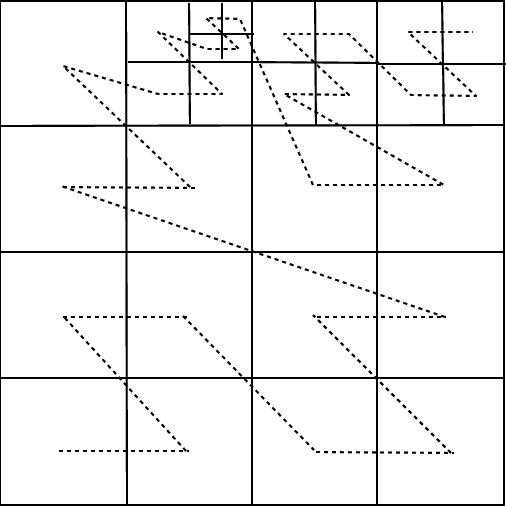
\includegraphics[width=3in]{Grid_f3}
\caption{\label{Fig:f3}
        Morton space-filling curve for adaptive mesh grids.}
\end{center}
\end{figure}

During the distribution step, each block is assigned a weight which
estimates the relative amount of time required to update the block.
The Morton number of the block is then
computed by interleaving the bits of its integer coordinates,
as described by Warren and Salmon (1987).  This reordering determines its
location along the space-filling curve.
Finally, the list of all
blocks is partitioned among the processors using the block weights,
equalizing the estimated workload of each processor.  By default, all leaf-blocks 
are weighted twice as heavily as all other blocks in the simulation.


%------------------------------------------------------------------------
% Refinement routines
%------------------------------------------------------------------------
\subsubsection{Specialized Refinement Routines}
\label{Sec:MarkRefLib}
Sometimes, it may be desirable to refine a particular region of
the grid independent of the second derivative of the variables.
This criterion might be, for example, to better resolve the flow at the
boundaries of the domain, to refine a region where there is vigorous
nuclear burning, or to better resolve some smooth initial condition.
For curvilinear coordinates, regions around the coordinate origin
or the polar $z$-axis may require special consideration for refinement.
A collection of methods that can refine a (logically) rectangular region
or a circular region in Cartesian coordinates, or can automatically
refine by using some variable threshold, are available through the 
\api{Grid/Grid_markRefineSpecialized}.
It  is intended to be called from 
 the \api{Grid/Grid_markRefineDerefine} routine.  The interface works
by allowing the calling routine to pick one of the routines in the
suite through an integer argument. The calling routine is also
expected to populate the data structure \code{specs} before making the
call. A copy of the file \code{Grid\_markRefineDerefine.F90} should be
placed in the \code{Simulation} directory, and the interface
file \code{Grid_interface.F90} should be used
in the header of the function.



\section{GridMain Usage}
\label{Sec:usage}

The \unit{Grid} unit has the largest API of all units, since it is the
custodian of the bulk of the simulation data, and is responsible for most
of the code housekeeping. The \api{Grid/Grid_init} routine, like all
other \code{Unit\_init} routines, collects the runtime parameters needed by
the unit and stores values in the data module. If using UG, the
\api{Grid/Grid_init} also creates the computational domain and the
housekeeping data structures and
initializes them. If using AMR, the computational domain is created
by the \api{Grid/Grid_initDomain} routine, which also makes a call to
mesh package's own initialization routine. The physical variables are all
owned by the \unit{Grid} unit, and it initializes them by
calling the \api{Simulation/Simulation_initBlock}
routine which applies the specified initial conditions to the
domain. If using an adaptive grid, the initialization routine also goes
through a few refinement iterations to bring the grid to desired
initial resolution, and then applies the \api{physics/Eos/Eos}
function to bring all simulation variables to thermodynamic equilibrium.
Even though the mesh-based variables are under \unit{Grid}'s control,
all the physics units can operate on and modify them.

A suite of \code{get/put} accessor/mutator functions allows the
calling unit to fetch or send data by the block. One option is to get a pointer
\api{Grid/Grid_getBlkPtr}, which gives unrestricted access to the whole
block and the client unit can modify the data as needed. The more
conservative but slower option is to get some portion of the block
data, make a local copy, operate on and modify the local copy and then
send the data back through the ``put'' functions. The \unit{Grid} interface
allows the client units to fetch the whole block
(\api{Grid/Grid_getBlkData}), a partial or full plane from a block
(\api{Grid/Grid_getPlaneData}), a partial or full row
(\api{Grid/Grid_getRowData}), or a single point
(\api{Grid/Grid_getPointData}). Corresponding ``put'' functions allow
the data to be sent back to the \unit{Grid} unit after the calling
routine has operated on it. Various \code{getData} functions can also
be used to fetch some derived quantities such as the cell volume or
face area of individual cells or groups of cells. There are several
other accessor functions available to query the housekeeping
information from the grid. For example \api{Grid/Grid_getListOfBlocks}
returns a list of blocks that meet the specified criterion such as
being ``LEAF'' blocks in \Paramesh, or residing on the physical
boundary. 


In addition to the functions to access the data, the \unit{Grid} unit also
provides a collection of routines that drive some housekeeping
functions of the grid without explicitly fetching any data. A good
example of such routines is \api{Grid/Grid_fillGuardCells}. Here no
data transaction takes place between \unit{Grid} and the calling
unit. The calling unit simply instructs the \unit{Grid} unit that it is ready for
the guard cells to be updated, and doesn't concern itself with the
details. The \api{Grid/Grid_fillGuardCells} routine makes sure that all the
blocks get the right data in their guardcells from their neighbors,
whether they are at the same, lower or higher resolution, and if
instructed by the calling routine, also ensures that \code{EOS} is
applied to them.

In large-scale, highly parallel Flash-X simulations with AMR, the processing
of \code{Grid\_fillGuardCells} calls may take up a significant part of
available resource like CPU time, communication bandwidth, and buffer space.
It can therefore be important to optimize these calls in particular.
From \flashx, \api{Grid/\-Grid_fillGuardCells} provides ways to
\begin{itemize}
\item operate on only a subset of the variables in \code{unk}
(and \code{facevarx}, \code{facevary}, and \code{facevarz}),
by masking out other variables;
\item fill only some the \code{nguard} layers of guard cells
that surround the interior of a block (while possibly excepting a ``sweep''
direction);
\item combine guard cell filling with EOS calls (which often follow
guard cell exchanges in the normal flow of execution of a simulation
in order to ensure thermodynamical consistency in all cells, and which
may also be very expensive), by letting \code{Grid\_fillGuardCells} 
make the calls on cells where necessary;
\item automatically determine masks and whether to call EOS, based on
the set of variables that the calling code actually needs updated.
by masking out other variables.
\end{itemize}
These options are controlled by \code{OPTIONAL} arguments, see
\api{Grid/Grid_fillGuardCells} for documentation.
When these optional arguments are absent or when a \unit{Grid}
implementation does not support them, Flash-X falls back to
safe default behavior which may, however, be needlessly expensive.

Another routine that may change the global state of the grid is
\api{Grid/Grid_updateRefinement}. This function is called
when the client unit wishes to update the grid's resolution. again,
the calling unit  does not need to know any of the details of the
refinement process.

\begin{flashtip}
As mentioned in \chpref{Chp:Architecture}, Flash-X allows every unit
to identify scalar variables for checkpointing. In the \unit{Grid} unit, the
function that takes care of consolidating user specified checkpoint
variable is \api{Grid/Grid_sendOutputData}. Users can select their own
variables to checkpoint by including an implementation of this
function specific to their requirements in their Simulation setup directory.
\end{flashtip}

%------------------------------------------------------------------------
% GridParticles - text in separate file.
%------------------------------------------------------------------------
%using \input because of LaTeX Error: \include cannot be nested.



\section{\unit{GridParticles}}
\label{Sec:GridParticles}

Flash-X is primarily an Eulerian code, however, there is support for
tracing the flow using Lagrangian particles. In \flashx we have
generalized the interfaces in the Lagrangian framework of the Grid
unit in such a way that it can also be used for miscellaneous 
non-Eulerian data such as tracing the path of a ray through the domain, 
or tracking the motion of solid bodies immersed in the fluid. Flash-X also
uses active particles with mass in cosmological simulations, and
charged particles in a hybrid PIC solver. Each particle has an
associated data structure, which contains fields such as its physical
position and velocity, and relevant physical attributes such as mass
or field values in active  particles. Depending upon the time advance
method, there may be other fields to store intermediate values. Also,
depending upon the requirements of the simulation, other physical variables
such as temperature \etc~ may be added to the data structure.
The \unit{GridParticles} subunit of the \unit{Grid} unit has two
sub-subunits of its own. The \unit{GridParticlesMove} sub-subunit 
moves the data structures associated with individual particles when
the particles move between blocks; the actual movement of the
particles through time advancement is the responsibility of the
\unit{Particles} unit. Particles move from one block to another
when their time advance places them outside their current
block. In AMR, the particles can also change their block through the
process of refinement and derefinement. The \unit{GridParticlesMap}
sub-subunit provides mapping between particles data and the mesh
variables. The mesh variables are either cell-centered or
face-centered, whereas a particle's position could be anywhere in the
cell. The \unit{GridParticlesMap} sub-subunit calculates the particle's
properties at its position from the corresponding mesh variable values
in the appropriate cell . When using active particles, this sub-subunit
also maps the mass of the particles onto the specified mesh variable
in appropriate cells.   The next sections describe the
algorithms for moving and mapping particles data.


\subsection{GridParticlesMove}
\label{Sec:GridParticlesMove}
\flashx has implementations of three different parallel algorithms
for moving the particles data when they are displaced from their
current block. \flashx had an additional algorithm, \code{Perfect
  Tree Level} which made use of the oct-tree structure. However,
because in all performance experiments it performed significantly
worse than the other two algorithms, it is not supported currently in
\flashx. The simplest algorithm, \code{Directional algorithm} is  
applicable only to the uniform grid when it is configured with one
block per processor. This algorithm uses directional movement of data,
and is easy because the directional neighbors are trivially known. 
The movement of particles data is much more challenging with AMR even
when the grid is not refining. Since the blocks are at various
levels of refinement at any given moment, a block may have more than one
neighbor along one or more of its faces. The distribution of blocks
based on space-filling curve is an added complication since the
neighboring blocks along a face may reside at a non-neighboring processor
The remaining two algorithmss included in \flashx implement
\code{GridParticlesMove} subunit for the adaptive mesh;  \code{Point
 to Point} and \code{Sieve}, of which only the \code{Sieve} algorithm
is able to move the data when the mesh refines. Thus even when a user
opts for the \code{PointToPoint} implementation for moving particles
with time evolution, some part of the \code{Sieve} implementation must
necessarily be included to  successfully move the data upon
refinement.   

\subsubsection{Directional Move}
\label{Sec: ug_algorithm}
The Directional Move algorithm for moving particles in a Uniform Grid 
minimizes the number of communication steps instead of minimizing
the volume of data moved. Its implementation has the following steps:
\begin{enumerate}
\item Scan particle positions.  Place all particles with their $x$
coordinate value greater than the block bounding box in the Rightmove
bin, and place those with $x$ coordinate less than block bounding box in
Leftmove bin.
\item Exchange contents of Rightbin with the right block neighbor's Leftbin
contents, and those of the Leftbin with left neightbor's Rightbin
contents.
\item Merge newly arrived particles from step 2 with those which did not move outside their original block.
\item Repeat steps 1-3 for the y direction.
\item Repeat step 1-2 for the z direaction.
\end {enumerate}

At the end of these steps, all particles will have reached their
destination blocks, including those that move to a neighbor on the
corner. \figref{Fig:ugMoveParticle} illustrates the steps in getting
a particle to its correct destination.
\begin{figure}
\begin{center}
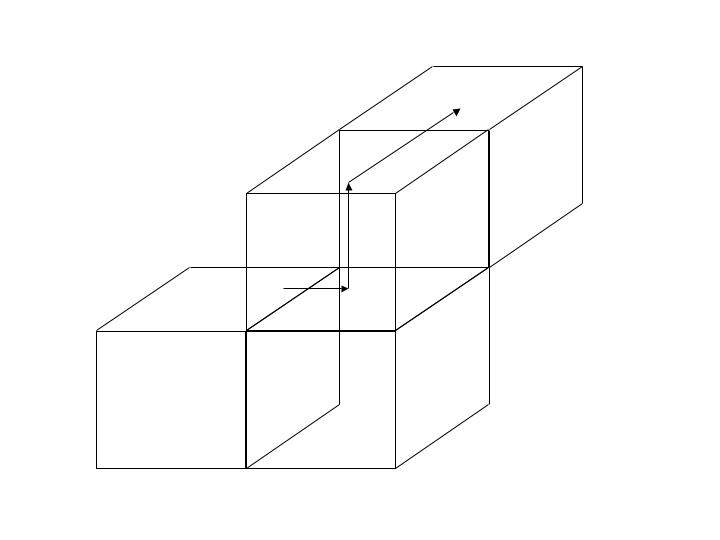
\includegraphics[width=3in]{Grid_ugMoveParticle}
\caption{\label{Fig:ugMoveParticle}
        Moving one particle to a neighbor on the corner.}
\end{center}
\end{figure}

\subsubsection {Point To Point Algorithm}
\label {Sec: ptop_algorithm}

As a part of the data cached by Paramesh, there is wealth of
information about the neighborhood of all the blocks on a
processor. This information includes the processor and block number of
all neighbors (face and corners) if they are at the same refinement
level. If those neighbors are at lower refinement level, then the
neighbor block is in reality the current block's parent's neighbor,
and the parent's neighborhood information is part of the cached
data. Similarly, if the neighbor is at a higher resolution then the
current blocks neighbor is in reality the parent of the neighbor. The
parent's metadata is also cached, from which information about all of
its children can be derived. Thus it is possible to determine the
processor and block number of the destination block for each particle.
The PointToPoint implementation finds out the destinations for every
particles that is getting displaced from its block. Particles going to
local destination blocks are moved first. The remaining particles are
sorted based on their destination processor number, followed by a
couple of global operations that allow every processor to determine
the number of particles it is expected to receive from all of the
other processors. A processor then posts asynchronous receives for
every source processor that had at least one particle to send to
it. In the next step, the processor cycles through the sorted list of
particles and sends them to the appropriate destinations using
synchronous mode of communition. 

\subsubsection{Sieve Algorithm}
\label {Sec: sieve_algorithm}
The \code{Sieve} algorithm does not concern itself with the
configuration of the underlying mesh at any time. It 
also does not distinguish between data movements due to time evolution
or regridding, and is therefore the only usable implementation when
the particles are displaced as a consequence of mesh refinement. 
The sieve implementation works with two bins, one
collects particles that have to be moved off-processor, and the other
receives particles sent to it by other processors. The following steps
broadly describe the algorithm: 
\begin{enumerate}
\item For each particle, find if its current position is on the current block
\item If not, find if its current position is on another block on the
same processor. If it is move the particle to that block, otherwise
put it in the send bin.
\item Send contents of the send bin to the designated neighbor, and
receive contents of another neighbor's send bin into my receive bin.
\item Repeat step 2 on the contents of the receive bin, and step 3
until all particles are at their destination.
\item For every instance of step 3, the designated send and receive
neighbors are different from any of the previous steps.
\end{enumerate}
In this implementation, the trick is to use an algorithm to determine
neighbors in such a way that all the particles reach their destination
in minimal number of hops. Using $MyPE+n*(-1)^{n+1}$ as the
destination processor and $MyPE+n*(-1)^{n}$ as the source processor in
modulo $numProcs$ arithmetic meets the requirements. Here $MyPE$ is
the local processor number and $numProcs$ is the number of processors.

% \subsubsection{Perfect Tree Level Algorithm}
% \label{Sec: perfectTree_algorithm}
% \code{PerfectTreeLevel} implementation exploits the oct-tree structure
% to move the data when there is no refinement. The algorithm can be
% written in four simple steps. 
% \begin {enumerate} 
% \item identify particles leaving the block
% \item move those particles up the oct-tree until they reach a level
% that is full (the level where all nodes exist)
% \item At this point the grid is reduced to Uniform Grid, apply the
% algorithm described in \secref{Sec: ug_algorithm}.
% \item move the newly arrived particles back down the tree to the
% appropriate leaves.
% \end {enumerate}
% Since each block contains complete information about its parent, and
% children it is relatively easy to navigate the
% tree. \figref{Fig:AMRParticlesNoRefine} shows the steps in the algorithm.

% \begin{figure}
% \begin{center}
% \includegraphics[width=3in]{Grid_AMRParticlesNoRefine}
% \caption{\label{Fig:AMRParticlesNoRefine}
%         Moving particles in AMR Grid when there is no refinement.}
% \end{center}
% \end{figure}


\subsection{GridParticlesMapToMesh}
\label{Sec:GridParticlesMapToMesh}
\flashx provides support for particles that can experience forces
and contribute to the problem dynamics.  These are termed
\emph{active} particles, and are described in detail in
\chpref{Chp:Particles}.  As these particles may move independently of
fluid flow, it is necessary to update the grid by mapping an attribute
of the particles to the cells of the grid.  We use these routines, for
example, during the PM method to assign the particles' mass to the
particle density solution variable \code{pden}. The hybrid PIC method 
uses its own variation for mapping appropriate physical quantities to
the mesh.

In general the mapping is performed using the grid routines in the
\code{GridParticlesMapToMesh} directory and the particle routines in
the \code{ParticlesMapping} directory.  Here, the particle subroutines
map the particles' attribute into a temporary array which is
independent of the current state of the grid, and the grid subroutines
accumulate the mapping from the array into valid cells of the
computational domain.  This means the grid subroutines accumulate the data
according to the grid block layout, the block refinement details, and
the simulation boundary conditions.  As these details are closely tied
with the underlying grid, there are separate implementations of the
grid mapping routines for UG and \Paramesh simulations.

The implementations are required to communicate information in a
relatively non-standard way.  Generally, domain decomposition parallel
programs do not write to the guard cells of a block, and only use the
guard cells to represent a sufficient section of the domain for the
current calculation.  To repeat the calculation for the next time
step, the values in the guard cells are refreshed by taking updated
values from the internal section of the relevant block.

In contrast, the guard cell values are mutable in the particle mapping
problem.  Here, it is possible that a portion of the particle's
attribute is accumulated in a guard cell which represents an internal
cell of another block.  This means the value in the updated guard cell
must be communicated to the appropriate block.  Unfortunately, the
mechanism to communicate information in this direction is not provided
by \Paramesh or UG grid.  As such, the relevant communication is
performed within the grid mapping subroutines directly.

In both \Paramesh and UG implementations, the particles' attribute is
``smeared'' across a temporary array by the generic particle mapping
subroutine.  Here, the temporary array represents a single leaf block
from the local processor.  In simulations using the \Paramesh grid,
the temporary array represents each LEAF block from the local
processor in turn.  We assign a particle's attribute to the temporary array when that
particle exists in the same space as the current leaf block.  For
details about the attribute assignment schemes available to the
particle mapping sub-unit, please refer to \secref{Sec:Particles
Mapping}.  

%Note that the particles are sorted in block
%order in the \Paramesh implementation, as this allows the particle
%mapping to be performed on a block by block basis.

After particle assignment, the \unit{Grid} sub-unit applies
simulation boundary conditions to those temporary arrays that
represent blocks next to external boundaries.  This may change the
quantity and location of particle assignment in the elements of the
temporary array.  The final step in the process involves accumulating
values from the temporary array into the correct cells of the
computational domain.  As mentioned previously, there are different
strategies for UG and \Paramesh grids, which are described in
\secref{Sec:UniformGridParticleMap} and
\secref{Sec:ParameshGridParticleMap}, respectively. 

\begin {flashtip}
The particle mapping routines can be run in a custom debug mode which
can help spot data errors (and even detect possible bugs).  In this
mode we inspect data for inconsistencies.  To use, append the
following line to the setup script:
\begin{codeseg}
-defines=DEBUG_GRIDMAPPARTICLES
\end{codeseg}
\end{flashtip}


\subsubsection{Uniform Grid}
\label{Sec:UniformGridParticleMap}

The Uniform Grid algorithm for accumulating particles' attribute on
the grid is similar to the particle redistribution algorithm described
in \secref{Sec: ug_algorithm}.  We once again apply the concept of
directional movement to minimize the number of communication steps:

\begin {enumerate}
\item Take the accumulated temporary array and iterate over all
  elements that correspond to the x-axis guard cells of the low block
  face.  If a guard cell has been updated, determine its position in
  the neighboring block of the low block face.  Copy the guard cell
  value and a value which encodes the destination cell into the send
  buffer.  %Guard cell values that have been updated must be
  %communicated to the neighboring block of the low block face.
\item Send the buffer to the low-side processor, and receive a buffer
  from the high-side processor.  For processors next to a domain
  boundary assume periodic conditions because all processors must
  participate.  If the simulation does not have periodic boundary
  conditions, there is still periodic communication at the boundaries,
  but the send buffers do not contain data.
\item Iterate over the elements in the receive buffer and accumulate
  the values into the local temporary array at the designated cells.
  It is possible to accumulate values in cells that represent internal
  cells and guard cells.  A value accumulated in a guard cell will be
  repacked into the send buffer during the next directional (y or z)
  sweep.
\item Repeat steps 1-3 for the high block face.
\item Repeat steps 1-4 for the y-axis, and then the z-axis.
\end {enumerate}

When the guard cell's value is packed into the send buffer, a single
value is also packed which is a 1-dimensional representation of the
destination cell's N-dimensional position.  The value is obtained by using an
array equation similar to that used by a compiler when mapping an
array into contiguous memory.  The receiving processor applies a
reverse array equation to translate the value into N-dimensional
space.  The use of this communication protocol is designed to minimize
the message size.

At the end of communication, each local temporary buffer contains
accumulated values from guard cells of another block.  The temporary
buffer is then copied into the solution array.



\subsubsection{Paramesh Grid}
\label{Sec:ParameshGridParticleMap}

There are two implementations of the AMR algorithms for accumulating
particles' attribute on the grid. They are inspired by a particle
redistribution algorithms \code{Sieve} and \code{Point to Point}
described  in \secref{Sec: sieve_algorithm}  and \secref{Sec:
ptop_algorithm} respectively. 

The \code{MoveSieve} implementation of the mapping algorithm uses the
same back and forth communication pattern as \code{Sieve} to minimize
the number of message exchanges.  That is, processor $MyPE$ sends to
$MyPE+n*(-1)^{n+1}$ and receives from $MyPE+n*(-1)^{n}$, where, $MyPE$
is the local processor number and $n$ is the count of the buffer
exchange round.  As such, this communication pattern involves a
processor exchanging data with its nearest neighbor processors first.
This is appropriate here because the block distribution generated by
the space filling curve should be high in data locality, \ie,
nearest neighbor blocks should be placed  on the same processor or
nearest neighbor processors.  

Similarly, the \code{Point to Point} implementation of the mapping
algorithm exploits the cached neighborhood knowledge, and uses a
judicious combination of global communications with asynchronous
receives and synchronous sends, as described in \secref{Sec:
ptop_algorithm}. Other than their communication patterns, the two
implementations are very similar as described below.

\begin {enumerate}
\item Accumulate the temporary array values into the central section
 of the corresponding leaf block.
\item Divide the leaf block guard cells into guard cell regions.
  Determine whether the neighbor(s) to a particular guard cell region
  exist on the same processor.
\item If a neighbor exists on the same processor, the temporary
  array values are accumulated into the central cells of that leaf
  block.  If the neighbor exists off processor, all temporary array
  values corresponding to a single guard cell region are copied into a
  send buffer.  Metadata is also packed into the send buffer which
  describes the destination of the updated values.
\item Repeat steps 1-3 for each leaf block.
\item Carry out data exchange with off-processor destinations as
described in the \secref{Sec: sieve_algorithm} or \secref{Sec: ptop_algorithm}
\end {enumerate}


%Step 2 and 3 are quite involved and are explained in more detail in
%the following paragraphs.

The guard cell region decomposition described in Step 2 is illustrated
in \figref{Fig:Grid_guardCell_divide}.  Here, the clear regions correspond to guard cells and
the gray region corresponds to internal cells.  Each guard cell region
contains cells which correspond to the internal cells of a single
neighboring block at the same refinement.

\begin{figure}[!ht]
\begin{center}
{\leavevmode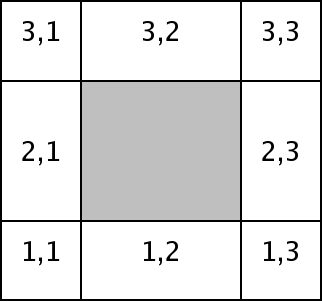
\includegraphics[width=3in]{Grid_guardCell_divide}}
\end{center}
\caption[Division of guard cells in 2-D block]{\label{Fig:Grid_guardCell_divide} A
single 2-D block showing how guard cells are divided into regions.}
\end{figure}

We use this decomposition as it makes it possible to query public
\Paramesh data structures which contain the block and process
identifier of the neighboring block at the same refinement.  However, at times
this is not enough information for finding the block neighbor(s) in a
refined grid.  We therefore categorize neighboring blocks as: Existing
on the same processor, existing on another processor and the block and
process ID are known, and existing on another processor and the block
and process ID are unknown.  If the block and process identifier are
unknown we use the \flashx corner ID.  This is a viable
alternative as the corner ID of a neighboring block can always be
determined.

The search process also identifies the refinement level of the
neighboring block(s).  This is important as the guard cell values
cannot be directly accumulated into the internal cells of another block
if the blocks are at a different refinement levels.  Instead the
values must be operated on in processes known as restriction and
prolongation (see \secref{Sec:gridinterp}).  We perform these
operations directly in the \code{GridParticlesMapToMesh} routines, and
use quadratic interpolation during prolongation.

Guard cell data is accumulated in blocks existing on the same
processor, or packed into a send buffer ready for communication.  When
packed into the send buffer, we keep values belonging to the same
guard cell region together.  This enables us to describe a whole
region of guard cell data by a small amount of metadata.  The metadata
consists of: Destination block ID, destination processor ID, block
refinement level difference, destination block corner ID (IAXIS,
JAXIS, KAXIS) and start and end coordinates of destination cells
(IAXIS, JAXIS, KAXIS).  This is a valid technique because there are no
gaps in the guard cell region, and is sufficient information for a
receiving processor to unpack the guard cell data correctly.

%The guard cell region is serialized into the send buffer in a similar
%way to \secref{Sec:UniformGridParticleMap}.  Here though, we choose to
%describe the entire guard cell region by 
%start and end coordinates for efficiency, rather than describing each
%guard cell individually.  This technique is valid as there are no gaps
%in the guard cell region.
%In order to use such an equation
%for an array, the array must be contiguous in memory.  This is not the
%case for a guard cell region, however, it can be applied because we do
%not need an actual mapping to a memory address.  All that is needed is
%a mapping to a unique 1-dimensional address, which can then be
%translated by the receiving processor into the desired N-dimensional
%cell address.  We therefore describe the entire guard cell region by 
%start and end coordinates for efficiency, rather than describing each
%guard cell individually.

We size the send / receive buffers according to the amount of data
that needs to be communicated between processors.  This is dependent
upon how the \Paramesh library distributes blocks to processors.
Therefore, in order to size the communication buffers economically, we
calculate the number of guard cells that will accumulate on blocks
belonging to another processor.  This involves iterating over every
single guard cell region, and keeping a running total of the number of
off-processor guard cells.  This total is added to the metadata total
to give the size of the send buffer required on each processor.  We use the maximum of the
send buffer size across all processors as the local size for the send
/ receive buffer.  Choosing the maximum possible size prevents
possible buffer overflow when an intermediate processor passes data
onto another processor.

After the point to point communication in step 6, the receiving
processor scans the destination processor identifier contained in each
metadata block.  If the data belongs to this processor it is unpacked
and accumulated into the central cells of the relevant leaf block.  As
mentioned earlier, it is possible that some guard cell sections do not
have the block and processor identifier.  When this happens, the
receiving processor attempts to find the same corner ID in one of its
blocks by performing a linear search over each of its leaf blocks.
Should there be a match, the guard cells are copied into the matched
block.  If there is no match, the guard cells are copied from the receive
buffer into the send buffer, along with any guard cell region
explicitly designated for another processor.  The packing and
unpacking will continue until all send buffers are empty, as indicated
by the result of the collective communication.

It may seem that the algorithm is unnecessarily complicated, however,
it is the only viable algorithm when the block and process identifiers
of the nearest block neighbors are unknown.  This is the situation in
\flashx.0, in which some data describing block and process
identifiers are yet to be extracted from \Paramesh.  
As an aside, this is different to the strategy used in Flash-X2, in
which the entire \Paramesh tree structure was copied onto each
processor.  Keeping a local copy of the entire \Paramesh tree
structure on each processor is an unscalable approach because increase
in the levels of resolution increases the meta-data memory overhead,
which restricts the size of  active particle simulations.  Therefore,
Point to Point method is a better option for
larger simulations, and significantly, simulations that run on
massively parallel processing (MPP) hardware architectures. 

In \flashx.1 we added a routine which searches non-public \Paramesh
data to obtain {\bf all} neighboring block and process identifiers.  This
discovery greatly improves the particle mapping performance because we
no longer need to perform local searches on each processor for blocks
matching a particular corner ID.

As another consequence of this discovery, we are able to experiment
with alternative mapping algorithms that require all block and process
IDs.  From \flashx.1 on we also provide a non-blocking point
to point implementation in which off-processor cells are sent directly
to the appropriate processor.  Here, processors receive messages at
incremented positions along a data buffer.  These messages can be
received in any order, and their position in the data buffer can
change from run to run.  This is very significant because the mass
accumulation on a particular cell can occur in any order, and
therefore can result in machine precision discrepancies.  Please be
aware that this can actually lead to slight variations in end-results
between two runs of the exact same simulation.  

% Finally, this
% implementation (under PttoPt subdirectory) is a proof on concept, and
% is not well tested compared to the MoveSieve implementation described
% earlier.  Also, we have no  results showing the relative performance
% of each implementation. 


%The particle positions and velocities at the next time step are calculated by
%considering both the long range and short range forces.
%The long range gravitational force between all particles is calculated 
%according to the particle-mesh (PM) technique.  In this technique, the
%gravitational acceleration on the mesh is used to update the positions and
%velocities of each particle.  
%The first stage in the technique is to 
%assign the particles' mass onto the mesh.  This gives
%a mesh-mapped particle density field in the particle density solution variable (pden).
%There are two different algorithms available for the mass assignment,
%one for UG simulations and one for \Paramesh simulations.

%This allows us to
%deduce the section in the guard cell region that needs to be copied to
%the block neighbor, and the section in the block neighbor that will
%receive the accumulated values.  


%\subsection{Example units to request}
%The stages in the PM technique and units required in 
%the Orbit simulation are as follows:
%1. Assign particles' mass to the mesh using an interpolation scheme. Different
%interpolation schemes are used depending on their accuracy and computational
%cost. The default scheme in Flash-X is Cloud-In-Cell (CIC).

%REQUESTS Particles\/ParticlesMapping\/meshWeighting\/CIC

%2. Solve Poisson's equation on the mesh in order to obtain the
%   gravitational potential.

%REQUESTS physics\/Gravity\/GravityMain\/Poisson\/Multigrid

%3. Perform a finite difference of the gravitational potential to obtain the force at each
%mesh cell.  Interpolate the forces from the cells to the particle positions
%using the same scheme as stage 1.

%REQUESTS Particles\/ParticlesMain\/active\/longRange\/gravity\/ParticleMesh

%4. Advance the particles' position and velocity.

%REQUESTS Particles\/ParticlesMain\/LeapfrogActive

 \section{GridSolvers}
\label{Sec:Solvers}


%-----------------------------------------------------------------------------
The \code{GridSolvers} unit groups together subunits that are used
to solve particular types of differential equations.  Currently, there
are two types of solvers:  a parallel Fast Fourier Transform package (\secref{Sec:GridSolversPfft})
and various solvers for the Poisson equation (\secref{Sec:GridSolversPoisson}).


%-----------------------------------------------------------------------------
\subsection {Pfft}
\label{Sec:GridSolversPfft}
\code{Pfft} is a parallel frame work for computing a Fast Fourier
Transform (FFT) on uniform grids. It can also be combined with the
Multigrid solver described below in \secref{Sec:GridSolversMultigrid} 
to let the composite solver scale to thousands of processors. 

\code{Pfft} has a layered architecture where the lower layer contains
functions implementing basic tasks and primary data structures.  The
upper layer combines pieces from the lowest layer to interface with Flash-X 
and create the parallel transforms. The computational part
of \code{Pfft} is handled by sequential 1-dimensional FFT's, which can be
from a native, vendor supplied scientific library, or from public
domain packages. The current distribution of Flash-X uses \code{fftpack} from
NCAR for the 1-D FFTs, since that package also contains transforms
that are useful with non-periodic boundary conditions. 

The lowest layer has three distinct components.  
The first component  redistributes data. 
It includes routines for distributed transposes
for two and three dimensional data. The second component provides a
uniform interface for FFT calls to hide the details of individual
libraries.  The third component is the data structures. There are global
data structures to keep track of the type of transform, number of data
dimensions, and physical and transform space information about each
dimension. The dimensional information 
includes the start and end point of data 
(useful when the dimension is spread over more than one processor), 
the MPI communicator, the coordinates of the node in
the processor grid etc. The structures also include pointers to the trigonometric
tables and work space needed by the sequential FFT calls. 

The upper layer of PFFT combines the lower layer routines to create
end-to-end transforms in a variety of ways. The available one
dimensional transforms include real-to-complex, complex-to-complex,
sine and cosine transforms. They can be combined to create two or
three dimensional tranforms for different configuration of the domain.
The two dimensional transforms support parallelization of one
dimension (or a one dimensional grid of  processors). 
The three dimensional transforms support one or two dimensional grid of
processors. All transforms must have at least one dimension within the
processor at all times. The data distribution changes during the
computation. However, a complete cycle of forward and inverse
transform restores the data distribution. 

The computation of a forward three dimensional FFT in parallel involves 
following steps :   
\begin {enumerate}
\item Compute 1-D transforms along {\bf x}.
\item Reorder, or transpose from {\bf x-y-z} to {\bf y-z-x}
\item Compute 1-D  transforms along {\bf y}. If the transform along
{\bf x} was real-to-complex, this one must be a complex-to-complex transform.
\item Transpose from {\bf y-z-x} to {\bf z-x-y}
\item Compute 1-D FFTs along {\bf z}. If the transform along {\bf x}
or {\bf y} was real-to-complex, this must be a complex-to-complex transform.
\end {enumerate} 

The inverse transform can be computed by carrying out the steps
described above in reverse order. The more commonly used domain
decomposition in FFT based codes assumes a one dimensional processor grid:

\begin {equation}\label {Eqn:Pfft_slab}
 N_1 \times N_2 \times N_3/P, 
\end {equation} 
where $N_1 \times N_2 \times N_3$ is the  global data size and $P$ is
the number of processors. Here, the first transpose is local, while
the second one is distributed. The internode communication is limited
to one distributed transpose involving all the processors. However,
there are two distinct disadvantages of this distribution  of work: 
\begin {itemize}
\item  The size of the problem imposes an upper limit on the number of 
processors, in that the largest individual dimension is also the
largest number of active processors. A three dimensional problem
is forced to  have modest individual dimensions to fit in the
processor memory.
\item As the machine size grows, the internode exchanges become long
range, and the possibility of contention grows.
\end {itemize}
We have chosen a domain decomposition where each subdomain is a column
of size \begin {eqnarray} \label {Eqn:Pfft_col}
N_1 \times N_2/P_1 \times N_3/P_2 \\ 
P = P_1 \times P_2. \nonumber
\end {eqnarray} 
With this distribution both the transposes are distributed in
parallel. The data exchange along any one processor grid dimension is
a collection of disjointed distributed transposes. Here, the
contention and communication range is reduced, while the volume of
data exchange is unaltered.  The distributed transposes are
implemented using collective {\bf MPI} operation {\bf alltoall}. In a
slabwise distribution, the upper limit on the number of processors is
determined by the smallest of $<N_1,N_2,N_3>$, where as in our
distribution, the upper limit on the number of processors is the
smallest of $<N_1*N_2,N_2*N_3,N_1*N_3>$. 

\subsubsection{Using \code{Pfft}}
\label{Sec:GridSolversUsingPfft}
\code{Pfft} can only be used with a pencil grid, with the constraint
that the number of processors along the \code{IAXIS} must be 1. This
is because all one dimensional transforms are computed locally within
a processor.  However, Flash-X contains a set of data
movement subroutines that generate a usable pencil grid from any UG
grid or any level of a PM grid.  These routines are briefly explained
in Section \ref{Sec:PFFTDataMove}.

During the course of a simulation, \code{Pfft} can be used in two
different modes. In the first mode, every instance of Pfft use will be
exactly identical to every other instance in terms of domain size and
the type of transforms. In this mode, the user can set the runtime
parameter \rpi{Grid/pfft_setupOnce} to true, which enables the
\code{Flash-X} initialization process to also create and initialize all
the data structures of \code{Pfft}. The finalization of the
\code{Pfft} subunit is also done automatically by the \code{Flash-X}
shutdown process in this mode. However, if a simulation needs to use
\code{Pfft} in different configurations at different instances of its
use, then each set of calls to \api{Grid/Grid_pfft} for computing the
transforms must be preceded by a call to \api{Grid/Grid_pfftInit} and
followed by a call to \api{Grid/Grid_pfftFinalize}. In addition, the
runtime parameter \rpi{Grid/pfft_setupOnce} should be set to false.  A
few other helper routines are available in the subunit to allow the
user to query \code{Pfft} about the dimensioning of the domain, and
also to map the Mesh variables from the \code{unk} array to and from
\code{Pfft} compatible (single dimensional) arrays.  \code{Pfft} also
provides the location of wave numbers in the parallel domain;
information that users can utilize to develop their own customized PDE
solvers using FFT based techniques.

\subsubsection{\code{Pfft} data movement subroutines}
\label{Sec:PFFTDataMove}
Mesh reconfiguration subroutines are available to generate a pencil
grid for the \code{Pfft} unit from another mesh configuration.  Two different implementations are
available at
\code{Grid/\-GridSolvers/\-Pfft/\-MeshReconfiguration/\-PtToPt} and
\code{Grid/\-GridSolvers/\-Pfft/\-MeshReconfiguration/\-Collective},
with the \code{PtToPt} implementation being the default.  Both
implementations are able to generate an appropriate pencil grid in UG
and PM mode.  The pencil processor grid is automatically selected, but
can be overridden by passing optional arguments to
\code{Grid_pfftInit}.  In UG mode they are invoked when the number of
processors in the \code{IAXIS} of the \code{Flash-X} grid is greater than one,
and in PM mode they are always invoked.  In PM mode they generate a
pencil grid from a single level of the AMR grid, which may be manually
specified or automatically selected as the maximum level that is
fully-refined (i.e. has blocks that completely cover the computational
domain at this level).

The pencil grid processor topology is stored in an \code{MPI}
communicator, and the communicator may contain fewer processors than are used in the
simulation.  This is to ensure the pencil grid points are never
distributed too finely over the processors, and naturally handles the 
case where the user may wish to obtain a pencil grid at a very coarse
level in the AMR grid.  If there are more blocks
than processors then we are safe to distribute the pencil grid over
{\bf all} processors, otherwise we must remove a number of processors.
Currently, we eliminate those processors that own {\bf zero} \code{Flash-X}
blocks at this level, as this is a simple calculation that can be
computed locally.

Both mesh reconfiguration implementations generate a map describing 
the data movement before moving any grid data.  The map is 
retained between calls to the \code{Pfft} routines and is 
only regenerated when the grid changes.  This avoids repeating 
the same global communications, but means communication buffers are
left allocated between calls to \code{Pfft}.

In the \code{Collective} 
implementation, the map coordinates are used to specify where 
the \code{Flash-X} data is copied into a send communication buffer.  Two 
\code{MPI_Alltoall} calls then move this data to the appropriate
pencil processor at coordinates (J,K).  Here, the first \code{MPI_Alltoall} moves data 
to processor (J,0), and the second \code{MPI_Alltoall} moves data 
to processor (J,K).  The decision to use \code{MPI_Alltoalls}
simplifies the \code{MPI} communication, but leads to very large 
send / receive communication buffers on each processor which consume:

\begin{verbatim}
Memory(bytes) = sizeof(REAL) * total grid points at solve level * 2
\end{verbatim}

The \code{PtToPt} implementation consumes less memory compared to the
\code{Collective} implementation, and communicates using point to
point \code{MPI} messages.  It is based upon using nodes in a linked
list which contain metadata (a map) and a communication buffer for a
single block fragment.  There are two linked lists: one for the
\code{Flash-X} block fragments and one for \code{Pfft} block fragments.
Metadata information about each \code{Flash-X} block fragment is placed
in separate messages and sent using \code{MPI_Isend} to the
appropriate destination pencil grid processor.

Each destination pencil grid processor repeatedly invokes
\code{MPI_Iprobe} using \code{MPI_ANY_SOURCE}, and creates a node in
its \code{Pfft} list whenever it discovers a message.  The \code{MPI}
message is received into a metadata region of the freshly allocated
node, and a communication buffer is also allocated according to the
size specified in the metadata.  The pencil processor continues
probing for messages until the cumulative size of its node's
communication buffers is equal to the pencil grid points it has been
assigned.  At this stage, grid data is communicated by traversing the
\code{Pfft} list and posting \code{MPI_Irecvs}, and then traversing
the \code{Flash-X} list and sending block fragment using
\code{MPI_Isends}.  After performing \code{MPI_Waits}, the received data in the 
nodes of the \code{Pfft} list is copied into internal \code{Pfft} arrays.

Note, the linked list is constructed using an include file stored at
\code{flashUtilities/\-datastructures/\-linkedlist}.  The file is named
\code{ut_listMethods.includeF90} and is meant to be included in any
\code{Fortran90} module to create lists with nodes of
a user-defined type.  Please see the README file, and the unit test
example at \code{flashUtilities/\-datastructures/\-linkedlist/\-UnitTest}.


\subsubsection{Unit Test}
\label{Sec:GridSolversPfftUnitTests}

The unit test for Pfft solver solves the following equation:
\begin{equation}
\label{Eqn:pfft Poisson}
\nabla^2({\bf F})=-13.0*\cos2x*\sin3y
\end{equation}
The simplest analytical solution of this equation assuming no
constants is
\begin{equation}
F=\cos2x*\sin3y
\end{equation}
We discretize the domain by assuming $xmin,ymin,zmin=0$, and
$xmax,ymax,zmax=2\pi$. The equation satisfies periodic boundary
conditions in this formulation and FFT based poisson solve techniques
can be applied. In the unit test we initialize one variable of the
solution data with the function $F$, and another one
with the right hand side of  \eqref{Eqn:pfft Poisson}. We
compute the forward real-to-complex transform of the solution data
variable that is initialized with the right hand side of \eqref{Eqn:pfft
Poisson}.  This variable is then divided by  
$({k_i}^2+{k_j}^2+{k_k}^2)$ where ${k_i, k_j}$ and ${k_k}$ are the
wavenumbers at any point {i,j,k} in the domain. An inverse complex-to-real
transform after the division should give the function $F$ as
result. Hence the unit test is considered successful if both the
variables have matching values within the specified tolerance.

\subsection{Poisson equation}
\label{Sec:GridSolversPoisson}

The \code{GridSolvers} subunit contains several different algorithms
for solving the general Poisson equation for a potential $\phi({\bf
x})$ given a source $\rho({\bf x})$ 
\begin{equation}
\label{Eqn:general Poisson}
\nabla^2\phi({\bf x}) = \alpha\rho({\bf x})\ .
\end{equation}
Here $\alpha$ is a constant that depends upon the application.  For example,
when the gravitational Poisson equation is being solved, $\rho({\bf x})$ is
the mass density, $\phi({\bf x})$ is the gravitational potential, and
$\alpha = 4\pi G$, where $G$ is Newton's gravitational constant.







\subsubsection{Multipole Poisson solver (original version)}
\label{Sec:GridSolversMultipole}
This section describes the multipole Poisson solver that has been
included in all the past releases of Flash-X. It is included in the
current release also, however, certain limitations found in this
solver lead to a new implementation described in
\secref{Sec:GridSolversMultipoleImproved}. This version is retained in
\flashx, because the new version is missing 
the ability to treat a non-zero minimal radius for spherical
geometries and the ability to specify a point mass contribution to the
potential. This will be implemented for the next coming release. 

The multipole Poisson solver is appropriate for spherical or nearly-spherical
source distributions with isolated boundary conditions (M{\"u}ller (1995)).
It currently works in 1D and 2D spherical, 2D axisymmetric cylindrical ($r,z$), and
3D Cartesian and axisymmetric geometries. Because of the imposed symmetries,
in the 1D spherical case, only the monopole term ($\ell = 0$) makes sense,
while in the axisymmetric and 2D spherical cases, only the $m = 0$ moments are used (\ie, the
basis functions are Legendre polynomials).

The multipole algorithm consists of the following steps.
First, find the center of mass ${\bf x}_{\rm cm}$
\begin{equation}
{\bf x}_{\rm cm} = {\int d^3{\bf x}\,{\bf x}\rho({\bf x}) \over
                    \int d^3{\bf x}\,\rho({\bf x})}\ .
\end{equation}
We will take ${\bf x}_{\rm cm}$ as our origin.  In integral form, Poisson's
(\eqref{Eqn:general Poisson}) is
\begin{equation}
\label{Eqn:Poisson integral}
\phi({\bf x}) = -{\alpha\over 4\pi}\int d^3{\bf x}'\,{\rho({\bf x}')\over
                |{\bf x} - {\bf x}'|}\ .
\end{equation}
The Green's function for this equation satisfies the relationship
\begin{equation}
\label{Eqn:Green}
{1\over |{\bf x} - {\bf x}'|} =
  4\pi\sum_{\ell=0}^\infty \sum_{m=-\ell}^\ell {1\over 2\ell+1}
  {r_<^\ell\over r_>^{\ell+1}}
  Y_{\ell m}^*(\theta',\varphi') Y_{\ell m}(\theta,\varphi)\ ,
\end{equation}
where the components of ${\bf x}$ and ${\bf x}'$ are expressed in
spherical coordinates $(r,\theta,\varphi)$ about ${\bf x}_{\rm cm}$, and
\begin{eqnarray}
r_< &\equiv& \min\{ |{\bf x}|, |{\bf x}'| \} \\
\nonumber
r_> &\equiv& \max\{ |{\bf x}|, |{\bf x}'| \}\ .
\end{eqnarray}
Here $Y_{\ell m}(\theta,\varphi)$ are the spherical harmonic functions
\begin{equation}
Y_{\ell m}(\theta,\varphi) \equiv
  (-1)^m \sqrt{ {2\ell+1\over 4\pi} {(\ell-m)!\over (\ell+m)!} }
  P_{\ell m}(\cos\theta) e^{im\varphi}\ .
\end{equation}
$P_{\ell m}(x)$ are Legendre polynomials.
Substituting \eqref{Eqn:Green} into
\eqref{Eqn:Poisson integral}, we obtain
\begin{eqnarray}
\label{Eqn:Multipole_poisint2}
\phi({\bf x}) &=& -\alpha
  \sum_{\ell=0}^\infty \sum_{m=-\ell}^\ell {1\over 2\ell+1}
  \Biggl\{
  Y_{\ell m}(\theta,\varphi) \times \\
\nonumber
  &&
  \left[ r^\ell \int_{r<r'} d^3{\bf x}' {\rho({\bf x}')
                   Y_{\ell m}^*(\theta',\varphi')\over {r'}^{\ell+1}} +
         {1\over r^{\ell+1}} \int_{r>r'} d^3{\bf x}' \rho({\bf x}')
                   Y_{\ell m}^*(\theta',\varphi') {r'}^\ell \right]\Biggr\} \ .
\end{eqnarray}
In practice, we carry out the first summation
up to some limiting multipole $\ell_{\rm max}$.
By taking spherical harmonic expansions about the center of mass, we
ensure that the expansions are dominated by low-multipole terms, so
that for a given value of $\ell_{\rm max}$, the error created by
neglecting high-multipole terms is minimized.
Note that the product of spherical harmonics in \eqref{Eqn:Multipole_poisint2} is
real-valued
\begin{eqnarray}
\sum_{m=-\ell}^\ell Y_{\ell m}^*(\theta',\varphi') Y_{\ell m}(\theta,\varphi)&=&
  {2\ell+1\over 4\pi} \Biggl[ P_{\ell 0}(\cos\theta) P_{\ell 0}(\cos\theta') +
  \\
\nonumber
  &&
  2\sum_{m=1}^\ell {(\ell-m)!\over (\ell+m)!}
  P_{\ell m}(\cos\theta)P_{\ell m}(\cos\theta')
  \cos\left(m(\varphi-\varphi')\right)
  \Biggr]\ .
\end{eqnarray}
Using a trigonometric identity to split up the last cosine in this expression
and substituting for the inner sums in \eqref{Eqn:Multipole_poisint2},
we obtain
\begin{eqnarray}
\label{Eqn:multipole potential}
\nonumber
\phi({\bf x}) &=& -{\alpha\over 4\pi}
                   \sum_{\ell=0}^\infty P_{\ell 0}(\cos\theta)\left[
  r^\ell \mu^{\rm eo}_{\ell 0}(r) +
  {1\over r^{\ell+1}} \mu^{\rm ei}_{\ell 0}(r) \right] - \\
  &&
  {\alpha\over 2\pi}
  \sum_{\ell=1}^\infty \sum_{m=1}^\ell P_{\ell m}(\cos\theta)\biggl[
  (r^\ell \cos m\varphi) \mu^{\rm eo}_{\ell m}(r) +
  (r^\ell \sin m\varphi) \mu^{\rm oo}_{\ell m}(r) + \\
\nonumber
  &&\qquad\qquad\qquad\qquad\qquad
  {\cos m\varphi\over r^{\ell+1}} \mu^{\rm ei}_{\ell m}(r) +
  {\sin m\varphi\over r^{\ell+1}} \mu^{\rm oi}_{\ell m}(r) \biggr]\ .
\end{eqnarray}
The even (e)/odd (o), inner (i)/outer (o) source moments in this expression are
defined to be
\begin{eqnarray}
\label{Eqn:moments1}
\mu^{\rm ei}_{\ell m}(r) &\equiv&
  {(\ell-m)!\over (\ell+m)!} \int_{r>r'} d^3{\bf x}'\,
  {r'}^\ell \rho({\bf x}') P_{\ell m}(\cos\theta') \cos m\varphi' \\
\mu^{\rm oi}_{\ell m}(r) &\equiv&
  {(\ell-m)!\over (\ell+m)!} \int_{r>r'} d^3{\bf x}'\,
  {r'}^\ell \rho({\bf x}') P_{\ell m}(\cos\theta') \sin m\varphi' \\
\mu^{\rm eo}_{\ell m}(r) &\equiv&
  {(\ell-m)!\over (\ell+m)!} \int_{r<r'} d^3{\bf x}'\,
  {\rho({\bf x}')\over {r'}^{\ell+1}} P_{\ell m}(\cos\theta') \cos m\varphi'
  \\
\label{Eqn:moments4}
\mu^{\rm oo}_{\ell m}(r) &\equiv&
  {(\ell-m)!\over (\ell+m)!} \int_{r<r'} d^3{\bf x}'\,
  {\rho({\bf x}')\over {r'}^{\ell+1}} P_{\ell m}(\cos\theta') \sin m\varphi'
  \ .
\end{eqnarray}
The procedure is thus to compute the moment integrals 
(\eqref{Eqn:moments1} $-$ \eqref{Eqn:moments4})
for a given source field $\rho({\bf x})$, and then to use these moments
in \eqref{Eqn:multipole potential} to compute the
potential.

In practice, the above procedure must take account of the fact that the
source and the potential are assumed to be cell-averaged
quantities discretized on a block-structured mesh with varying cell size.
Also, because of the radial dependence of the multipole moments of the
source function, these moments must be tabulated as functions of distance from
${\bf x}_{\rm cm}$, with an implied discretization.  The solver allocates
storage for moment samples spaced a distance $\Delta$ apart in radius
\begin{eqnarray}
\mu^{\rm ei}_{\ell m,q}\equiv \mu^{\rm ei}_{\ell m}(q\Delta) &&
\mu^{\rm eo}_{\ell m,q}\equiv \mu^{\rm eo}_{\ell m}((q-1)\Delta) \\
\mu^{\rm oi}_{\ell m,q}\equiv \mu^{\rm oi}_{\ell m}(q\Delta) &&
\mu^{\rm oo}_{\ell m,q}\equiv \mu^{\rm oo}_{\ell m}((q-1)\Delta)\ .
\end{eqnarray}
The sample index $q$ varies from 0 to $N_q$ ($\mu^{\rm eo}_{\ell m,0}$ and
$\mu^{\rm oo}_{\ell m,0}$ are not used).  The sample spacing $\Delta$ is
chosen to be one-half the geometric mean of the $x$, $y$, and $z$ cell spacings
at the highest level of refinement, and $N_q$ is chosen to be large enough
to span the diagonal of the computational volume with samples.

Determining the contribution of individual
cells to the tabulated moments requires some care.  To reduce the error
caused by the grid geometry, in each cell $ijk$
an optional subgrid can be establish (see \rpi{Grid/mpole_subSample})
consisting of $N'$ points at the locations
${\bf x}'_{i'j'k'}$, where
\begin{eqnarray}
x'_{i'} = x_i + (i'-0.5(N'-1)){\Delta x_i\over {N'}}\ ,&&
  i' = 0\ldots {N'}-1 \\
y'_{j'} = y_j + (j'-0.5(N'-1)){\Delta y_j\over {N'}}\ ,&&
  j' = 0\ldots {N'}-1 \\
z'_{k'} = z_k + (k'-0.5(N'-1)){\Delta z_k\over {N'}}\ ,&&
  k' = 0\ldots {N'}-1 \ ,
\end{eqnarray}
and where ${\bf x}_{ijk}$ is the center of cell $ijk$.  (For clarity, we have
omitted $ijk$ indices on ${\bf x}'$ as well as all block indices.)
For each subcell, we assume $\rho({\bf x}'_{i'j'k'})\approx\rho_{ijk}$
and then apply
\begin{eqnarray}
\label{Eqn:discmoments1}
\mu^{\rm ei}_{\ell m,q\ge q'} &\leftarrow& \mu^{\rm ei}_{\ell m,q\ge q'} +
  {(\ell-m)!\over (\ell+m)!} {\Delta x_i\Delta y_j\Delta z_k\over {N'}^3}
  {r'}_{i'j'k'}^\ell \rho({\bf x}'_{i'j'k'}) P_{\ell m}(\cos\theta'_{i'j'k'})
  \cos m\varphi'_{i'j'k'} \\
\mu^{\rm oi}_{\ell m,q\ge q'} &\leftarrow& \mu^{\rm oi}_{\ell m,q\ge q'} +
  {(\ell-m)!\over (\ell+m)!} {\Delta x_i\Delta y_j\Delta z_k\over {N'}^3}
  {r'}_{i'j'k'}^\ell \rho({\bf x}'_{i'j'k'}) P_{\ell m}(\cos\theta'_{i'j'k'})
  \sin m\varphi'_{i'j'k'} \\
\mu^{\rm eo}_{\ell m,q\le q'} &\leftarrow& \mu^{\rm eo}_{\ell m,q\le q'} +
  {(\ell-m)!\over (\ell+m)!} {\Delta x_i\Delta y_j\Delta z_k\over {N'}^3}
  {\rho({\bf x}'_{i'j'k'})\over {r'}_{i'j'k'}^{\ell+1}}
  P_{\ell m}(\cos\theta'_{i'j'k'})
  \cos m\varphi'_{i'j'k'} \\
\label{Eqn:discmoments4}
\mu^{\rm oo}_{\ell m,q\le q'} &\leftarrow& \mu^{\rm oo}_{\ell m,q\le q'} +
  {(\ell-m)!\over (\ell+m)!} {\Delta x_i\Delta y_j\Delta z_k\over {N'}^3}
  {\rho({\bf x}'_{i'j'k'})\over {r'}_{i'j'k'}^{\ell+1}}
  P_{\ell m}(\cos\theta'_{i'j'k'}) \sin m\varphi'_{i'j'k'}
  \ ,
\end{eqnarray}
where
\begin{equation}
q' = \left\lfloor{|{\bf x}'_{i'j'k'} }| \over {\Delta}
     \right\rfloor + 1
\end{equation}
is the index of the radial sample within which the subcell center lies.
These expressions introduce (hopefully) small errors when compared to
(\eqref{Eqn:moments1}) $-$ (\ref{Eqn:moments4}), because the
subgrid volume elements are not spherical. These
errors are greatest when $r' \sim \Delta x$; hence, using a subgrid
reduces the amount of source affected by these errors.
An error of order $\Delta^2$ is also introduced by assuming the source
profile within each cell to be flat.
Note that the total source computed by this method ($\mu^{\rm ei}_{\ell m,N_q}$)
is exactly equal to the total implied by $\rho_{ijk}$.

Another way to reduce grid geometry errors when using the multipole
solver is to modify the AMR refinement criterion to refine all blocks
containing the center of mass (in addition to other criteria that may
be used, such as the second-derivative criterion supplied with \Paramesh).
This ensures that the center-of-mass point is maximally refined at all
times, further restricting the volume which contributes errors to the
moments because $r' \sim \Delta x$.

The default value of $N'$ is 1; note that large values of this
parameter very quickly increase the amount of time required to evaluate
the multipole moments (as ${N'}^3$). In order to speed up the moment
summations, the sines and cosines in
(\eqref{Eqn:discmoments1}) $-$ (\ref{Eqn:discmoments4}) are evaluated using
trigonometric recurrence relations, and the factorials are pre-computed
and stored at the beginning of the run.

When computing the cell-averaged potential, we again employ a subgrid, but
here the subgrid points fall on cell boundaries to improve the continuity
of the result.  Using $N'+1$ subgrid points per dimension, we have
\begin{eqnarray}
x'_{i'} = x_i + (i'-0.5N')){\Delta x_i\over {N'}}\ ,&&
  i' = 0\ldots {N'} \\
y'_{j'} = y_j + (j'-0.5N')){\Delta y_j\over {N'}}\ ,&&
  j' = 0\ldots {N'} \\
z'_{k'} = z_k + (k'-0.5N')){\Delta z_k\over {N'}}\ ,&&
  k' = 0\ldots {N'} \ .
\end{eqnarray}
The cell-averaged potential in cell $ijk$ is then
\begin{equation}
\phi_{ijk} = {1\over {N'}^3} \sum_{i'j'k'} \phi({\bf x}'_{i'j'k'})\ ,
\end{equation}
where the terms in the sum are evaluated via 
\eqref{Eqn:multipole potential} up to the limiting multipole order
$\ell_{\rm max}$.

\begin{comment}
\begin{flashtip}
In \flashx, two different parameters were available to control subsampling.
In \flashx, the sub-sampling is made consistent with the use of only one
runtime parameter \rpi{Grid/mpole_subSample} to avoid excessive wasted computation
in one section of the calculation.
The default value of \code{mpole_subSample} is 1; meaning no subsampling is performed
by default and the code runs much faster.  Should additional accuracy be required, increase
this runtime parameter.
\end{flashtip}
\end{comment}


\subsubsection{Multipole Poisson solver (improved version)}
\label{Sec:GridSolversMultipoleImproved}

The multipole Poisson solver is based on a multipolar expansion of the source (mass for gravity,
for example) distribution around a conveniently chosen center of expansion. The angular number
$L$ entering this expansion is a measure of how detailed the description of the source
distribution will be on an angular basis. Higher $L$ values mean higher angular resolution with
respect to the center of expansion. The multipole Poisson solver is thus appropriate for spherical
or nearly-spherical source distributions with isolated boundary conditions. For problems which
require high spatial resolution throughout the entire domain (like, for example, galaxy collision
simulations), the multipole Poisson solver is less suited, unless one is willing to go to extremely
(computationally unfeasible) high $L$ values. For stellar evolution, however, the multipole
Poisson solver is the method of choice.
\par
The new implementation of the multipole Poisson solver is located in the directory
\begin{codeseg}
source/Grid/GridSolvers/Multipole_new.
\end{codeseg}
This implementation improves upon the original implemention in many ways:
i) efficient memory layout 
ii) elimination of numerical over- and underflow
errors for large angular momenta when using astrophysical
(dimensions $\approx 10^9$) domains
iii) elimination of subroutine call overhead (1 call per cell),
iv) minimization of error due to non-statistical distributions of
moments near the multipolar origin. The following paragraphs explain
the new approach to the multipole solver and an explanation of the
above improvements. Details about the theory of the new implementation of the Poisson solver
can be found in Couch et al.~(2013).
\par
The multipole Poisson solver is appropriate for spherical or nearly-spherical
source distributions with isolated boundary conditions. It currently works in
1D spherical, 2D spherical, 2D cylindrical, 3D Cartesian and 3D cylindrical. Symmetries
can be specified for the 2D spherical and 2D cylindrical cases (a horizontal symmetry plane
along the radial axis) and the 3D Cartesian case (assumed axisymmetric property).
Because of the radial symmetry in the 1D spherical case, only the monopole term
($\ell = 0$) contributes, while for the 3D Cartesian axisymmetric, the 2D cylindrical
and 2D spherical cases only the $m = 0$ moments need to be used (the other $m\neq 0$
moments effectively cancel out).
\par
The multipole algorithm consists of the following steps. First, the center of
the multipolar expansion ${\bf x}_{\rm cen}$ is determined via density-squared weighted
integration over position:
\begin{equation}
{\bf x}_{\rm cen} = {\int {\bf x}\rho^2({\bf x})\,d{\bf x} \over
                    \int \rho^2({\bf x})\,d{\bf x}}.
\end{equation}
We will take ${\bf x}_{\rm cen}$ as our origin.  In integral form, Poisson's
equation (\ref{Eqn:general Poisson}) becomes
\begin{equation}
\label{Eqn:PoissonIntegral}
\phi({\bf x}) = -{\alpha\over 4\pi}\int {\rho({\bf x}')\over
                |{\bf x} - {\bf x}'|}\,d{\bf x}'.
\end{equation}
The inverse radial distance part can be expanded in terms of Legendre
polynomials
\begin{equation}
\label{Eqn:Inverse distance Legendre}
{1\over |{\bf x} - {\bf x}'|} = \sum_{\ell=0}^\infty
{x_<^\ell\over x_>^{\ell+1}}P_\ell (\cos\gamma),
\end{equation}
where $x_<$ ($x_>$) indicate the smaller (larger) of the magnitudes
and $\gamma$ denotes the angle between ${\bf x}$ and ${\bf x}'$. Note, that this
definition includes those cases where both magnitudes are equal. The expansion
is always convergent if $\cos\gamma <1$. Expansion of the Legendre polynomials
in terms of spherical harmonics gives
\begin{equation}
\label{Eqn:Legendre spherical harmonics}
P_\ell (\cos\gamma) = {4\pi\over 2\ell+1}\sum_{m=-\ell}^{+\ell}
Y_{\ell m}^*(\theta',\phi') Y_{\ell m}(\theta,\phi),
\end{equation}
where $\theta,\phi$ and $\theta',\phi'$ are the spherical angular components of
${\bf x}$ and ${\bf x}'$ about ${\bf x}_{\rm cen}$.
Defining now the regular $R_{\ell m}$ and irregular $I_{\ell m}$ solid
harmonic functions
\begin{eqnarray}
R_{\ell m}(x_<) & = & \sqrt{{4\pi\over {2\ell+1}}}x_<^\ell Y_{\ell m}(\theta,\phi) \\
I_{\ell m}(x_>) & = & \sqrt{{4\pi\over {2\ell+1}}}{Y_{\ell m}(\theta,\phi)\over x_>^{\ell+1}},
\end{eqnarray}
we can rewrite Eq.(\ref{Eqn:PoissonIntegral}) in the form
\begin{equation}
\label{Eqn:Poisson solid harmonics}
\phi({\bf x}) = -{\alpha\over 4\pi}
\int \sum_{\ell m}R_{\ell m}(x_<)I_{\ell m}^*(x_>)\rho({\bf x}')\,d{\bf x}',
\end{equation}
where the summation sign is a shorthand notation for the double sum over all the
allowed $\ell$ and $m$ values. In Flash-X both the source and the potential are
assumed to be cell-averaged quantities discretized on a block-structured mesh with
varying cell size. The integration must hence be replaced by a summation over all 
leaf cells
\begin{equation}
\label{Eqn:Poisson discrete incorrect}
\phi(q) = -{\alpha\over 4\pi}
\sum_{q'} \sum_{\ell m}R_{\ell m}(q_<)I_{\ell m}^*(q_>)m(q'),
\end{equation}
where $m$ denotes the cell's mass. Note, that the symbol $q$ stands for cell index as well
as its defining distance position from the expansion center in the computational domain.
This discrete Poisson equation is incorrect. It contains the divergent $q'=q$ term on
the rhs. The $q'=q$ contribution to the potential corresponds to the cell self potential
$\phi_{Self}(q)$ and is divergent in our case because all the cell's mass is assumed to be
concentrated at the cell's center. The value of this divergent term can easily be calculated
from Eq.(\ref{Eqn:Inverse distance Legendre}) by setting $\cos\gamma = 1$:
\begin{eqnarray}
\phi_{Self}(q) & = &  m(q){L+1\over x_q},
\end{eqnarray}
where $m$ is the cell's mass, $L$ the highest angular number considered in the expansion
and $x_q$ the radial distance of the cell center from the expansion center. To avoid this divergence
problem, we evaluate the potentials on each face of the cell and form the average of all
cell face potentials to get the cell center potential. Eq.(\ref{Eqn:Poisson discrete incorrect})
will thus be replaced by
\begin{equation}
\phi(q) = {1\over n_F} \sum_{F} \phi({\bf x}_F)
\end{equation}
and
\begin{equation}
\label{Eqn:Poisson discrete correct}
\phi({\bf x}_F) = -{\alpha\over 4\pi}
\sum_{q'} \sum_{\ell m}R_{\ell m}([q',x_F]_<)I_{\ell m}^*([q',x_F]_>)m(q'),
\end{equation}
where ${\bf x}_F$ is the cell face radial distance from the expansion center and $[q',x_F]_<$ denotes the
larger of the magnitudes between the cell center radial distance $q'$ and the cell face radial distance $x_F$.
Splitting the summation over cells in two parts
\begin{equation}
\label{Eqn:Poisson discrete correct 1}
\phi({\bf x}_F) = -{\alpha\over 4\pi}\left\{
\sum_{q'\leq x_F} \sum_{\ell m}\left[R_{\ell m}(q')m(q')\right]I_{\ell m}^*({\bf x}_F)
+ \sum_{q'>x_F} \sum_{\ell m}R_{\ell m}({\bf x}_F)\left[I_{\ell m}^*(q')m(q')\right]\right\},
\end{equation}
and defining the two moments
\begin{eqnarray}
M^R_{\ell m}({\bf x}_F) & = & \sum_{q'\leq x_F} R_{\ell m}(q')m(q') \label{Eqn:Moment definition 1} \\
M^I_{\ell m}({\bf x}_F) & = & \sum_{q'>x_F} I_{\ell m}(q')m(q'),\label{Eqn:Moment definition 2}
\end{eqnarray}
we obtain
\begin{equation}
\label{Eqn:Poisson discrete correct 2}
\phi({\bf x}_F) = -{\alpha\over 4\pi}\left[
\sum_{\ell m}M^R_{\ell m}({\bf x}_F)I_{\ell m}^*({\bf x}_F)
+ \sum_{\ell m}M^{I*}_{\ell m}({\bf x}_F)R_{\ell m}({\bf x}_F)\right]
\end{equation}
and using vector notation
\begin{equation}
\label{Eqn:Poisson discrete correct 3}
\phi({\bf x}_F) = -{\alpha\over 4\pi}\left[
{\bf M}^R({\bf x}_F)\cdot {\bf I}^*({\bf x}_F) + {\bf M}^{I*}({\bf x}_F)\cdot {\bf R}({\bf x}_F)
\right].
\end{equation}
\par
We now change from complex to real formulation. We state this for the regular
solid harmonic functions, the same reasoning being applied to the irregular
solid harmonic functions and all their derived moments. The regular solid
harmonic functions can be split into a real and imaginary part
\begin{equation}
\label{Eqn:Solid harmonics real}
R_{\ell m} = R_{\ell m}^c + i\,R_{\ell m}^s.
\end{equation} 
The labels 'c' and 's' are shorthand notations for 'cosine' and 'sine',
reflecting the nature of the azimuthal function of the corresponding real
spherical harmonics. When inserting (\ref{Eqn:Solid harmonics real}) into
(\ref{Eqn:Poisson discrete correct 3}) all cosine and sine mixed terms of the
scalar products cancel out. Also, due to the symmetry relations
\begin{eqnarray}
R_{\ell,-m}^c & = & (-1)^m R_{\ell m}^c \\
R_{\ell,-m}^s & = & -(-1)^m R_{\ell m}^s
\end{eqnarray} 
we can restrict ourselves to the following polar angle number ranges
\begin{eqnarray}
c & : & \ell\geq 0\;\;,\;\;\ell\geq m \geq 0 \\
s & : & \ell\geq 1\;\;,\;\;\ell\geq m \geq 1.
\end{eqnarray}
The real formulation of (\ref{Eqn:Poisson discrete correct 3}) becomes then
\begin{equation}
\label{Eqn:Poisson discrete correct real}
\phi({\bf x}_F) = -{\alpha\over 4\pi}\left\{
\left[\begin{array}{l}
{\bf M}^{Rc}({\bf x}_F) \\
{\bf M}^{Rs}({\bf x}_F)
\end{array}\right]
\cdot {\bf \Delta}
\left[\begin{array}{l}
{\bf I}^c({\bf x}_F) \\
{\bf I}^s({\bf x}_F)
\end{array}\right]
+
\left[\begin{array}{l}
{\bf M}^{Ic}({\bf x}_F) \\
{\bf M}^{Is}({\bf x}_F)
\end{array}\right]
\cdot {\bf \Delta}
\left[\begin{array}{l}
{\bf R}^c({\bf x}_F) \\
{\bf R}^s({\bf x}_F)
\end{array}\right]\right\},
\end{equation}
which, when compared to (\ref{Eqn:Poisson discrete correct 3}), shows, that all vectors now
contain a cosine and a sine section. The ${\bf \Delta}$ matrix is a diagonal matrix whose elements
are equal to 2 for $m\neq 0$ and 1 otherwise, i.e.:
\begin{equation}
\label{Eqn:Delta matrix}
{\bf \Delta} = diag(2-\delta_{m0}).
\end{equation}
The recursion relations for calculating the solid harmonic vectors are
\begin{eqnarray}
R_{00}^c & = & 1 \label{Eqn:Regular Recurrence} \\
R_{\ell\ell}^c & = & - {xR_{\ell-1,\ell-1}^c-yR_{\ell-1,\ell-1}^s\over 2\ell}\\
R_{\ell\ell}^s & = & - {yR_{\ell-1,\ell-1}^c+xR_{\ell-1,\ell-1}^s\over 2\ell}\\
R_{\ell m}^{c/s} & = & {(2\ell - 1)zR_{\ell-1,m}^{c/s}-r^2R_{\ell-2,m}^{c/s}
                       \over (\ell + m)(\ell - m)},\;\;\;0\leq m <\ell
\end{eqnarray}
and
\begin{eqnarray}
I_{00}^c & = & {1\over r} \\
I_{\ell\ell}^c & = & - (2\ell-1){xI_{\ell-1,\ell-1}^c-yI_{\ell-1,\ell-1}^s\over r^2} \\
I_{\ell\ell}^s & = & - (2\ell-1){yI_{\ell-1,\ell-1}^c+xI_{\ell-1,\ell-1}^s\over r^2} \\
I_{\ell m}^{c/s} & = & {(2\ell - 1)zI_{\ell-1,m}^{c/s}-\left[(\ell-1)^2-m^2\right]
                       I_{\ell-2,m}^{c/s}\over r^2},\;\;\;0\leq m <\ell
\label{Eqn:Irregular Recurrence}
\end{eqnarray}
in which $x,y,z$ are the cartesian location coordinates of the cell face and $r^2=x^2+y^2+z^2$.
For geometries depending on polar angles one must first calculate the corresponding cartesian
coordinates for each cell before applying the recursions. In Flash-X, the order of the two cosine
and sine components for each solid harmonic vector is such that $\ell$ precedes $m$.
This allows buildup of the vectors with maximum number of unit strides. The same
applies of course for the assembly of the moments. For 2D cylindrical and 2D spherical geometries
only the $m=0$ parts of both recursions are needed, involving only the cartesian $z$ coordinate
and $r^2$. Symmetry along the radial axes of these 2D geometries inflicts only the sign change
$z\rightarrow -z$, resulting in the symmetry relations $R_{\ell 0}^c\rightarrow R_{\ell 0}^c$ for
even $\ell$ and $R_{\ell 0}^c\rightarrow -R_{\ell 0}^c$ for odd $\ell$, the same holding for the
irregular solid harmonic vector components. Thus symmetry in 2D can effectively be treated
by halving the domain size and multiplying each even $\ell$ moments by a factor of 2 while setting
the odd $\ell$ moments equal to 0. For 3D cartesian geometries introduction of symmetry
is far more complicated since all $m$ components need to be taken into account. It is not
sufficient to simply reduce the domain to the appropriate size and multiply the moments
by some factor, but rather one would have to specify the exact symmetry operations intended
(generators of the symmetry group $O_h$ or one of its subgroups) in terms of their effects
on the $x,y,z$ cartesian basis. The resulting complications in calculating symmetry adapted moments
outweighs the computational gain that can be obtained from it. Options for 3D symmetry are
thus no longer available in the improved Flash-X multipole solver. The 'octant' symmetry option
from the old multipole solver, using only the monopole $\ell=0$ term, was too restrictive in
its applicability (exact only for up to angular momenta $\ell =3$ due to cancellation of the
solid harmonic vector components).
\par
From the above recursion relations (\ref{Eqn:Regular Recurrence}-\ref{Eqn:Irregular Recurrence}),
the solid harmonic vector components are functions
of $x^iy^jz^k$ monomials, where $i+j+k=\ell$ for the ${\bf R}$ and (formally)
$i+j+k=-(\ell+1)$ for the ${\bf I}$. For large astrophysical coordinates and large $\ell$ values this leads
to potential computational over- and underflow. To get independent of the size of both
the coordinates and $\ell$ we introduce a damping factor $Dx,Dy,Dz$ for the coordinates
for each solid harmonic type before entering the recursions. $D$ will be chosen such that for the
highest specified $\ell=L$ we will have approximately a value close to 1 for both
solid harmonic components:
\begin{eqnarray}
R^{c/s}_{Lm} & \approx & 1 \label{Eqn:Damping condition 1} \\
I^{c/s}_{Lm} & \approx & 1.\label{Eqn:Damping condition 2}
\end{eqnarray}
This ensures proper handling of size at the solid harmonic function evaluation level and one
does not have to rely on size cancellations at a later stage when evaluating the potential via
Eq.(\ref{Eqn:Poisson discrete correct real}). We next state the evaluation of the
damping factor $D$. Due to the complicated nature of the recursions, the first step is to
find solid harmonic components which have a simple structure. To do this, consider a cell
face with $x,y=0$ and $z\neq 0$. Then $r^2=z^2$, $|z|=r$ and only the $m=0$ components are
different from zero. An explicit form can be stated for the absolute values of these
components in terms of $r$:
\begin{eqnarray}
\label{Eqn:Regular solid harmonic xy0}
|R_{\ell 0}| & = & {r^\ell\over \ell!} \\
|I_{\ell 0}| & = & {\ell!\over r^{\ell+1}}. \label{Eqn:Irregular solid harmonic xy0}
\end{eqnarray}
Since $r=\sqrt{x^2+y^2+z^2}$, damping of the coordinates with $D$ results in a damped
radial cell face distance $Dr$. Inserting this result into (\ref{Eqn:Regular solid harmonic xy0})
and (\ref{Eqn:Irregular solid harmonic xy0})
and imposing conditions (\ref{Eqn:Damping condition 1}) and (\ref{Eqn:Damping condition 2})
results in
\begin{eqnarray}
\label{Eqn:Damping components}
D_R = {1\over r}\sqrt[L]{L!} & \approx & {1\over r}{L\over e}\sqrt[2L]{2\pi L}\\
D_I = {1\over r}\sqrt[L+1]{L!} & \approx & {1\over r}{L\over e}\sqrt[2L+2]{{2\pi e^2\over L}},
\end{eqnarray}
where the approximate forms are obtained by using Stirling's factorial approximation
formula for large $L$. In Flash-X only the approximate forms are computed for $D_R$ and $D_I$
to avoid having to deal with factorials of large numbers.
\par
From the moment defining equations (\ref{Eqn:Moment definition 1}) and (\ref{Eqn:Moment definition 2})
we see, that the moments are sums over subsets of cell center solid harmonic vectors multiplied
by the corresponding cell mass. From Eq.(\ref{Eqn:Poisson discrete correct real}) it follows that
for highest accuracy, the moments should be calculated and stored for each possible cell face.
For high refinement levels and/or 3D simulations this would result in an unmanageable request
for computer memory. Several cell face positions have to be bundled into radial bins $Q$ defined
by lower and upper radial bounds. Once a cell center solid harmonic vector pair ${\bf R}(q)$ and
${\bf I}(q)$ for a particular cell has been calculated, its radial bin location $q\rightarrow Q$
is determined and its contribution is added to the radial bin moments ${\bf M}^R(Q)$ and ${\bf M}^I(Q)$.
The computational definition of the radial bin moments is
\begin{eqnarray}
\label{Eqn:Moment computational definition}
{\bf M}^R(Q) & = & \sum_{q\leq Q}{\bf R}(q)m(q) \\
{\bf M}^I(Q) & = & \sum_{q\geq Q}{\bf I}(q)m(q),
\end{eqnarray}
where $q\leq Q$ means including all cells belonging to $Q$ and all radial bins
with lower radial boundaries than $Q$. The two basic operations of the multipole solver
are thus: i) assembly of the radial bin moments and ii) formation of the scalar
products via Eq.(\ref{Eqn:Poisson discrete correct real}) to obtain the potentials.
The memory declaration of the moment array should reflect the way the individual
moment components are addressed and the most efficient layout puts the angular momentum
indices in rows and the radial bin indices in columns.
\par
How do we extract moments ${\bf M}^R({\bf x})$ and ${\bf M}^I({\bf x})$ at any particular position
${\bf x}$ inside the domain (and, in particular, at the cell face positions ${\bf x}_F$), which are
ultimately needed for the potential evaluation at that location? Assume that the location
${\bf x}$ corresponds to a particular radial bin ${\bf x}\rightarrow Q$. Consider the
three consecutive radial bins $Q-1$, $Q$ and $Q+1$, together with their calculated moments:
\begin{equation}
\begin{array}{r|r|r}
{\bf M}^R(Q-1) & {\bf M}^R(Q) & {\bf M}^R(Q+1) \\
{\bf M}^I(Q-1) & {\bf M}^I(Q) & {\bf M}^I(Q+1)
\end{array}
\end{equation}
Let us concentrate on the $Q$ bin, whose lower and upper radial limits are shown
as solid vertical lines. The radial distance corresponding to ${\bf x}$ splits the
$Q$ bin into two parts: the left fractional part, denoted $R_{frac}$, and the right
fractional part, denoted $I_{frac}$. Since both ${\bf M}^R(Q-1)$ and ${\bf M}^I(Q+1)$
are completely contained respectively in ${\bf M}^R(Q)$ and ${\bf M}^I(Q)$, the
moments at ${\bf x}$ be approximately evaluated as:
\begin{eqnarray}
{\bf M}^R({\bf x}) & = &  {\bf M}^R(Q-1) + R_{frac}\left[{\bf M}^R(Q)-{\bf M}^R(Q-1)\right]
\label{Eqn:Cell moment computational definition 1} \\
{\bf M}^I({\bf x}) & = &  {\bf M}^I(Q+1) + I_{frac}\left[{\bf M}^I(Q)-{\bf M}^I(Q+1)\right],
\label{Eqn:Cell moment computational definition 2}
\end{eqnarray}
The extraction of the moments via (\ref{Eqn:Cell moment computational definition 1})
and (\ref{Eqn:Cell moment computational definition 2}) is
of course an approximation that relies on the statistically dense distribution of the individual
cell center moments inside each radial bin. For bins which are reasonably far away from the expansion
center this statistical approximation is valid but for those close to the expansion center the
statistical distribution does not hold and calculating the moments via the above scheme
introduces a large statistical error. The way out of this problem is to move from a statistical
radial bin description around the expansion center to a more discrete one, by constructing very narrow
isolated radial bins. The code is thus forced to analyze the detailed structure of the geometrical domain
grid surrounding the expansion center and to establish the inner radial zone of discrete distributed
radial bins. The statistical radial bins are then referred to as belonging to the outer radial zone(s).
\par
While the structure of the inner radial zone is fixed due to the underlying geometrical grid,
the size of each radial bin in the outer radial zones has to be specified by the user. There is
at the moment no automatic derivation of the optimum (accuracy vs memory cost)
bin size for the outer zones. There are two types of radial bin sizes defined for the Flash-X
multipole solver: i) exponentially and/or ii) logarthmically growing:
\begin{eqnarray}
\mbox{exponential bin size upper radial limit} & = & s\cdot \Delta r \cdot Q^t
\label{Eqn:Exponential bin definition} \\
\mbox{logarithmic bin size upper radial limit} & = & s\cdot \Delta r \cdot {e^{tQ}-1\over e^t-1}.
\label{Eqn:Logarithmic bin definition}
\end{eqnarray}
In these definitions, $\Delta r$ is a small distance 'atomic' (basic unit) radial measure, defined
as half the geometric mean of appropriate cell dimensions at highest refinement level, $s$ is a scalar factor
to optionally increase or decrase the atomic unit radial measure and $Q = 1,2,\ldots$ is a local bin
index counter for each outer zone. The atomic radial distance $\Delta r$ is calculated for each individual
domain geometry as follows:
\begin{eqnarray}
&&\begin{tabular}{c|c}
Domain Geometry & $\Delta r$ \\
\hline
3D cartesian   &  ${1\over 2}\sqrt[3]{\Delta x\Delta y\Delta z}$ \\
3D cylindrical &  ${1\over 2}\sqrt{\Delta R\Delta z}$ \\
2D cylindrical &  ${1\over 2}\sqrt{\Delta R\Delta z}$ \\
2D spherical   &  ${1\over 2}\Delta R$ \\
1D spherical   &  ${1\over 2}\Delta R$
\end{tabular},
\end{eqnarray}
where $\Delta x,\Delta y,\Delta z$ are the usual cartesian cell dimensions and $\Delta R$ is
the radial cell dimension. Note, that since $\Delta r$ measures a basic radial unit along the
radial distance from the expansion center (which, for approximate spherical problems, is located
close to the domain's geometrical origin), only those cell dimensions for calculating each
$\Delta r$ are taken, which are directly related to radial distances from the geometrical domain origin.
For 3D cylindrical domain geometries for example, only the radial cylindrical and z-coordinate
cell dimensions determine the 3D radial distance from the 3D cylindrical domain origin. The
angular coordinate is not needed. Likewise for spherical domains only the radial cell coordinate
is of importance. Definitions (\ref{Eqn:Exponential bin definition}) and
(\ref{Eqn:Logarithmic bin definition}) define the upper limit of the radial bins. Hence in order to
obtain the true bin size for the $Q$-th bin one has to subtract its upper radial limit from the
corresponding one of the $(Q-1)$-th bin:
\begin{eqnarray}
\mbox{$Q$-th exponential bin size} & = & s\cdot \Delta r \cdot \left[Q^t-(Q-1)^t\right] \\
\mbox{$Q$-th logarithmic bin size} & = & s\cdot \Delta r \cdot e^{t(Q-1)}.
\end{eqnarray}
In principle the user can specify as many outer zone types as he/she
likes, each having its own exponential or logarithmic parameter pair $\{s,t\}$.
\par
Multithreading of the code is currently enabled in two parts: 1) during moment evaluation and 2)
during potential evaluation. The threading in the moment evaluation section is achieved by
running multiple threads over separate, non-conflicting radial bin sections. Moment evaluation
is thus organized as a single loop over all relevant radial bins on each processor. Threading
over the potential evaluation is done over blocks, as these will address different non-conflicting
areas of the solution vector.
\par
The improved multipole solver was extensively tested and several runs have been performed
using large domains ($>10^{10}$) and extremely high angular numbers up to $L=100$ for a variety
of domain geometries. Currently, the following geometries can be handled: 3D cartesian,
3D cylindrical, 2D cylindrical, 2D spherical and 1D spherical. The structure of the code is
such that addition of new geometries, should they ever be needed by some applications,
can be done rapidly. 


\subsubsection{Multipole Poisson solver unit test (MacLaurin spheroid)}
\label{Sec:GridSolversMultipoleUnitTest1}

The first unit test for the multipole Poisson solver is based on the MacLaurin spheroid analytical
gravitational solution given in section \ref{Sec:SimulationMacLaurin}. The unit test sets up
a spheroid with uniform unit density and determines both the analytical and numerical gravitational
fields. The absolute relative error based on the analytical solution is formed for each cell
and the maximum of all the absolute errors is compared to a predefined error tolerance value
for a particular uniform refinement level. The multipole unit test runs in 2D cylindrical,
2D spherical, 3D cartesian and 3D cylindrical geometries and threaded multipole unit tests are
also available.

%\subsubsection{Multipole Poisson solver unit test (Rectangular Box)}
%\label{Sec:GridSolversMultipoleUnitTest2}
%
%The second unit test for the multipole Poisson solver is based on the uniform density rectangular
%box analytical gravitational solution. For a rectangular box of dimensions $x,y,z$ an analytical
%formula can be given for the self potential per unit mass at its midpoint
%$(x/2,y/2,z/2)$ in terms of inverse tangent and hyperbolic tangent functions, simplifying considerably
%for a cubic cell ($T$ being a shorthand notation for $1/\sqrt{x^2+y^2+z^2}$):
%\begin{eqnarray}
%\phi_{Self}(xyz)/m  & = & 2xy\;\artanh(Tz)+2xz\;\artanh(Ty)+2yz\;\artanh(Tx) \\
%                    &   & -x^2\;\arctan(yzT/x)-y^2\;\arctan(xzT/y)-z^2\;\arctan(xyT/z) \nonumber \\
%\phi_{Self}(cube)/m & = & 3x^2\left[2\;\artanh(1/\sqrt{3})-\;\arctan(1/\sqrt{3})\right] \\
%                    & \approx & 2.3800772\;x^2.
%\end{eqnarray}
%Here $T=1/\sqrt{x^2+y^2+z^2}$.

\subsubsection{Tree Poisson Solver}
\label{Sec:GridSolversBHTree}

The tree solver is based on the Barnes \& Hut (1986, Nature, 324, 446) tree code
for calculation of gravity forces in N-body simulations. However, it is more
general and it includes some more modern features described for instance in
Salmon \& Warren (1994, J. Comp. Phys, 136, 155), Springel (2005, MNRAS, 364,
1105) and other works. It builds a global octal tree over the whole
computational domain, communicates its part to all processors and uses it for
calculations of various physical problems provided as separate units in
source/physics directory. The global tree is an extension of the AMR mesh octal
tree down to individual cells. The communication of the tree is implemented so
that only parts of the tree that are needed for the calculation of the potential
on a given processor are sent to it. The calculation of physical problems is
done by walking the tree for each grid cell (hereafter {\em
point-of-calculation}) and evaluating whether the tree node should be used for
calculation or whether its children should be open.

The tree solver is connected to physical units by several wrapper subroutines
that are called at specific places of the tree build and tree walk, and that
call corresponding subroutines of physical units. In this way, physical
units can include arbitrary quantity into the tree, and then, use it to
calculate some other physical quantity by integrating contributions of all tree
nodes during the tree walk. In this version, the only working unit implementation is
\code{physics/Gravity/GravityMain/Poisson/BHTree}, which calculates the gravitational
potential.

The tree solver algorithm consists of four parts. The first one, communication of block
properties, is called only if the AMR grid changes. The other three, building of
the tree, communication of the tree and calculation of the potential, are called
in each time-step.

\textit{Communication of block properties.} In recent version, each processor
needs to know some basic information about all blocks in the simulation. It
includes arrays: \texttt{nodetype}, \texttt{lrefine} and \texttt{child}. These
arrays are distributed from each processor to all the other processors. They can
occupy a substantial amount of memory on large number of processors (memory
required for statically allocated arrays of the tree solver can be calculated by
a script \texttt{tree\_mem\_use.py}). 

\textit{Building the tree.} The global tree is constructed from bottom and the
process consists of three steps. In the first one, the so-called {\em
block-tree} is constructed in each leaf block on a given processor. The {\em
block-trees} are 1-dimensional dynamically allocated arrays (see
Figure~\ref{fig:btree}) and pointers to them are stored in array
\texttt{gr\_bhTreeArray}. In the second step, top nodes of block-trees
(corresponding to whole blocks) are distributed to all processors and stored in
array \texttt{gr\_bhTreeParentTree}. In the last step, higher nodes of the
parent tree are calculated by each processor and stored in the
\texttt{gr\_bhTreeParentTree} array. At the end, each processor holds
information about the global tree down to the level of leaf blocks. During the
whole process of tree building, 5 subroutines providing the interface to
physical units are called: \code{gr\_bhFillBotNode},
\code{gr\_bhAccBotNode}, \code{gr\_bhAccNode}, \code{gr\_bhNormalizeNode}
and \code{gr\_bhPostprocNode} (see their auto-documentation and source code
for details). Each of them calls a corresponding subroutine of all physical
units with a name where the first two letters 'gr' are replaced with the name
of the unit (e.g. \api{physics/Gravity/Gravity\_bhFillBotNode}).

\begin{figure}[h]
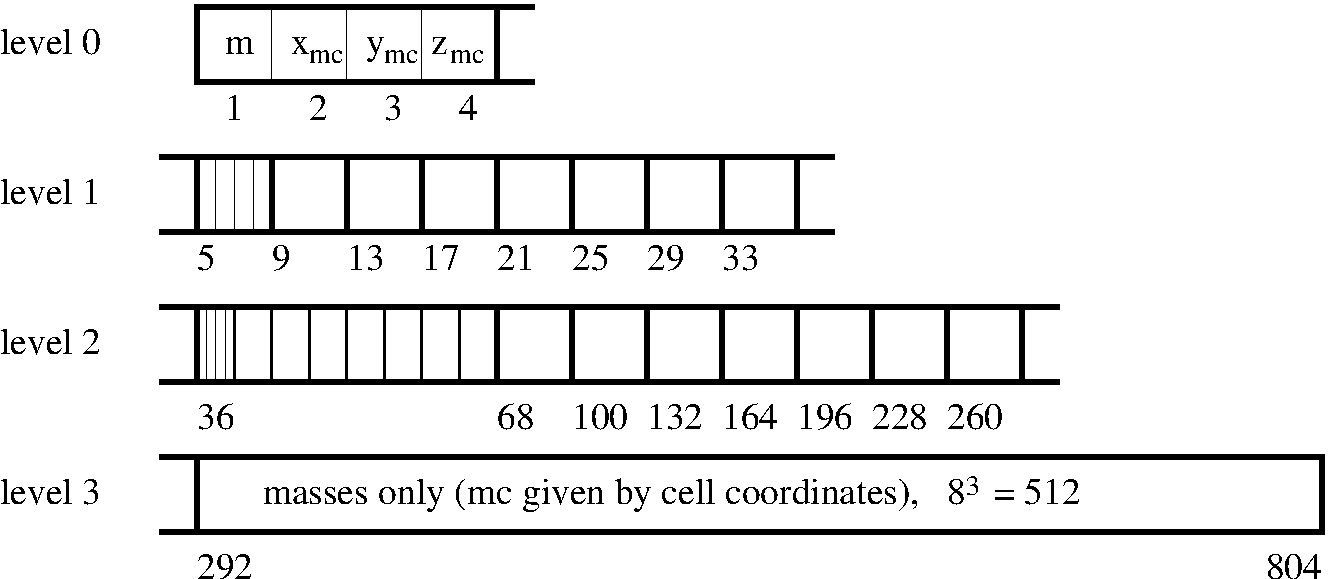
\includegraphics[width=15cm]{tree-in-ram}
\caption{Example of a {block-tree} in case of
\texttt{nxb}=\texttt{nyb}=\texttt{nzb}=8 and in case physical units do not
store any further information to tree nodes (masses and mass centre positions
are included by the tree solver itself).}
\label{fig:btree}
\end{figure}

\textit{Communication of the tree.} Most of the tree data is contained on the
bottom levels in individual {\em block-trees}. In order to save memory and
communication time, only parts of {\em block-trees} that are needed on a given
processor are sent to it. The procedure consists of three steps. In the first
one, a level down to which each {\em block-tree} has to be sent to each
processor is determined. For a given {\em block-tree}, it is done by evaluating
the criterion for the node acceptance (traditionally called multipole acceptance
criterion, shortly MAC) for all blocks on a remote processor, searching for the
maximum level down to which the evaluated node will be needed on a given remote
processor. In the second step, information about the {\em block-tree}
levels which are going to be communicated is sent to all processors. This
information is needed for allocation of arrays in which {\em block-trees} are
stored on remote processors. In the third step, the {\em block-tree} arrays are
allocated, all {\em block-trees} for a given processor are packed into a single
message and the messages are communicated.

The MAC is implemented in subroutine \code{gr\_bhMAC} which includes only a
simple geometrical MAC used also by Barnes \& Hut. The node is accepted for
calculation if
\begin{equation}
\label{eq:stl}
\frac{S_\mathrm{node}}{D} < \mathtt{gr\_bhTreeLimAngle} \ ,
\end{equation}
where $S_\mathrm{node}$ is the node size (defined as the largest edge of the
corresponding cuboid) and $D$ is the distance between the node and the {\em
point-of-calculation}. Additionally, \code{gr\_bhMAC} checks that the {\em
point-of-calculation} is not located within the node itself enlarged by factor
\rpi{Grid/gr\_bhTreeSafeBox}. On the top of that, \code{gr\_bhMAC} calls MACs of 
physical units and the node is accepted only if all criteria are fulfilled.

\textit{Tree walk.} The tree is traversed from the top to the bottom, evaluating
MAC of each node and in case it is not fulfilled, continuing the tree walk with
its children. If the node's MAC is fulfilled, the node is accepted for the
calculation and subroutine \code{gr\_bhBotNodeContrib} or
\code{gr\_bhNodeContrib} is called, depending on whether it is a bottom-most
node (i.e. a single grid cell) or higher node, respectively. These subroutines
only call the corresponding subroutines of physical units (\eg,
\texttt{Gravity\_bhNodeContrib}). This is the most CPU-intensive part of
the tree solver, it usually takes more than $90\%$ of the total tree solver
time. It is completely parallel and it does not include any communication (apart
from sending some statistics to the main processor at the end).

The tree solver includes several implementations of the tree walk. The default
algorithm is the Barnes-Hut like tree walk in which the whole tree is traversed
from the top down to nodes fulfilling MAC for each cell separately. This
algorithm is used in case the runtime parameter \rpi{Grid/gr\_bhUnifiedTreeWalk} is
true (default). If it this parameter is set to false, another algorithm is used
in which instead of walking the whole tree for each cell individually, MAC is at
first evaluated for whole mesh block (interacting with some node). If the node
is accepted and if the node is a parent node (i.e. corresponding to whole mesh
block), the node is accepted for all cells of the block and the contribution of
the node is added to them. However, the node contribution is calculated
separately for each cell, because the distance between the node and individual
cells differs. The third tree walk algorithm is an implementation of the so
called \texttt{SumSquare} MAC described by Salmon \& Warren (1994). The tree is
traversed using the priority queue, taking contribution of the most important
nodes first. This algorithm provides much better error control, however, the
implementation in this code version is highly experimental.

The tree solver supports isolated and periodic boundary conditions that can be
set independently in each direction. In the latter case, when a node is
considered for MAC evaluation and eventually calculation by calling
\api{physics/Gravity/Gravity\_bhNodeContrib}, periodic copies of the
node are checked, and the minimum distance among the node periodic copies is
taken in account. This allows for instance to calculate gravitational potential
with periodic boundary conditions using the Ewald method (see description of the
Gravity unit).


\subsubsection{Tree Poisson solver unit test}

The unit test for the tree gravity solver calculates the gravitational potential
of the Bonnor-Ebert sphere (Bonnor, W. B., 1956, MNRAS, 116, 351) and compares
it to the analytical potential. The density distribution and the analytical
potential are calculated by the python script \texttt{bes-generator.py}. The
simulation setup only reads the file with radial profiles of these quantities
and sets it on the grid. It also normalizes the analytical potential (adds a
constant to it) so that the minimum values of the analytical and numerical
potential are the same. The error of the gravitational potential calculated by
the tree code is stored in the field array PERR (written into the PlotFile). The
maximum absolute and relative errors are written into the log file.


%-------------------------------------------------------------------------------
%\input{GridSolversTreeWunsch.tex}  (old version)
%-------------------------------------------------------------------------------


\subsubsection{Multigrid Poisson solver}
\label{Sec:GridSolversMultigrid}

This section of the  User's Guide is taken from a paper by
Paul Ricker,
``A Direct Multigrid Poisson Solver for Oct-Tree Adaptive Meshes''
 (2008).  Dr. Ricker wrote an original version of this 
multigrid algorithm for \flashx.  The Flash Center adapted it to
\flashx.

Structured adaptive mesh refinement provides some challenges for the
implementation of effective, parallel multigrid methods.  In the case of
patch-based meshes, Huang \& Greengard (2000) presents an algorithm which works by
using the coarse-grid solution to impose boundary values on the fine grid.
Discontinuities in the solution caused by jumps in refinement are resolved
through iterative calculation of the residual and subsequent correction.  While
this is not a multigrid method in the standard sense, it still provides
significant convergence acceleration.

The adaptation of this method to the Flash-X grid structure (Ricker, 2008) requires a few
modifications.  The original formulation required that there be shared points
between the coarse and fine patches.  Contrast this with finite-volume,
nested-cell, cell-averaged grids as used in Flash-X(\figref{Fig:GridSolvers_hgMultigrid_f1}).  This is overcome by the
exchange of guardcells from coarse to fine using monotonic interpolation
(\secref{Sec:gridinterp}) and external boundary extrapolation for the calculation of
the residual.

\begin{figure}[!ht]
\begin{center}
{\leavevmode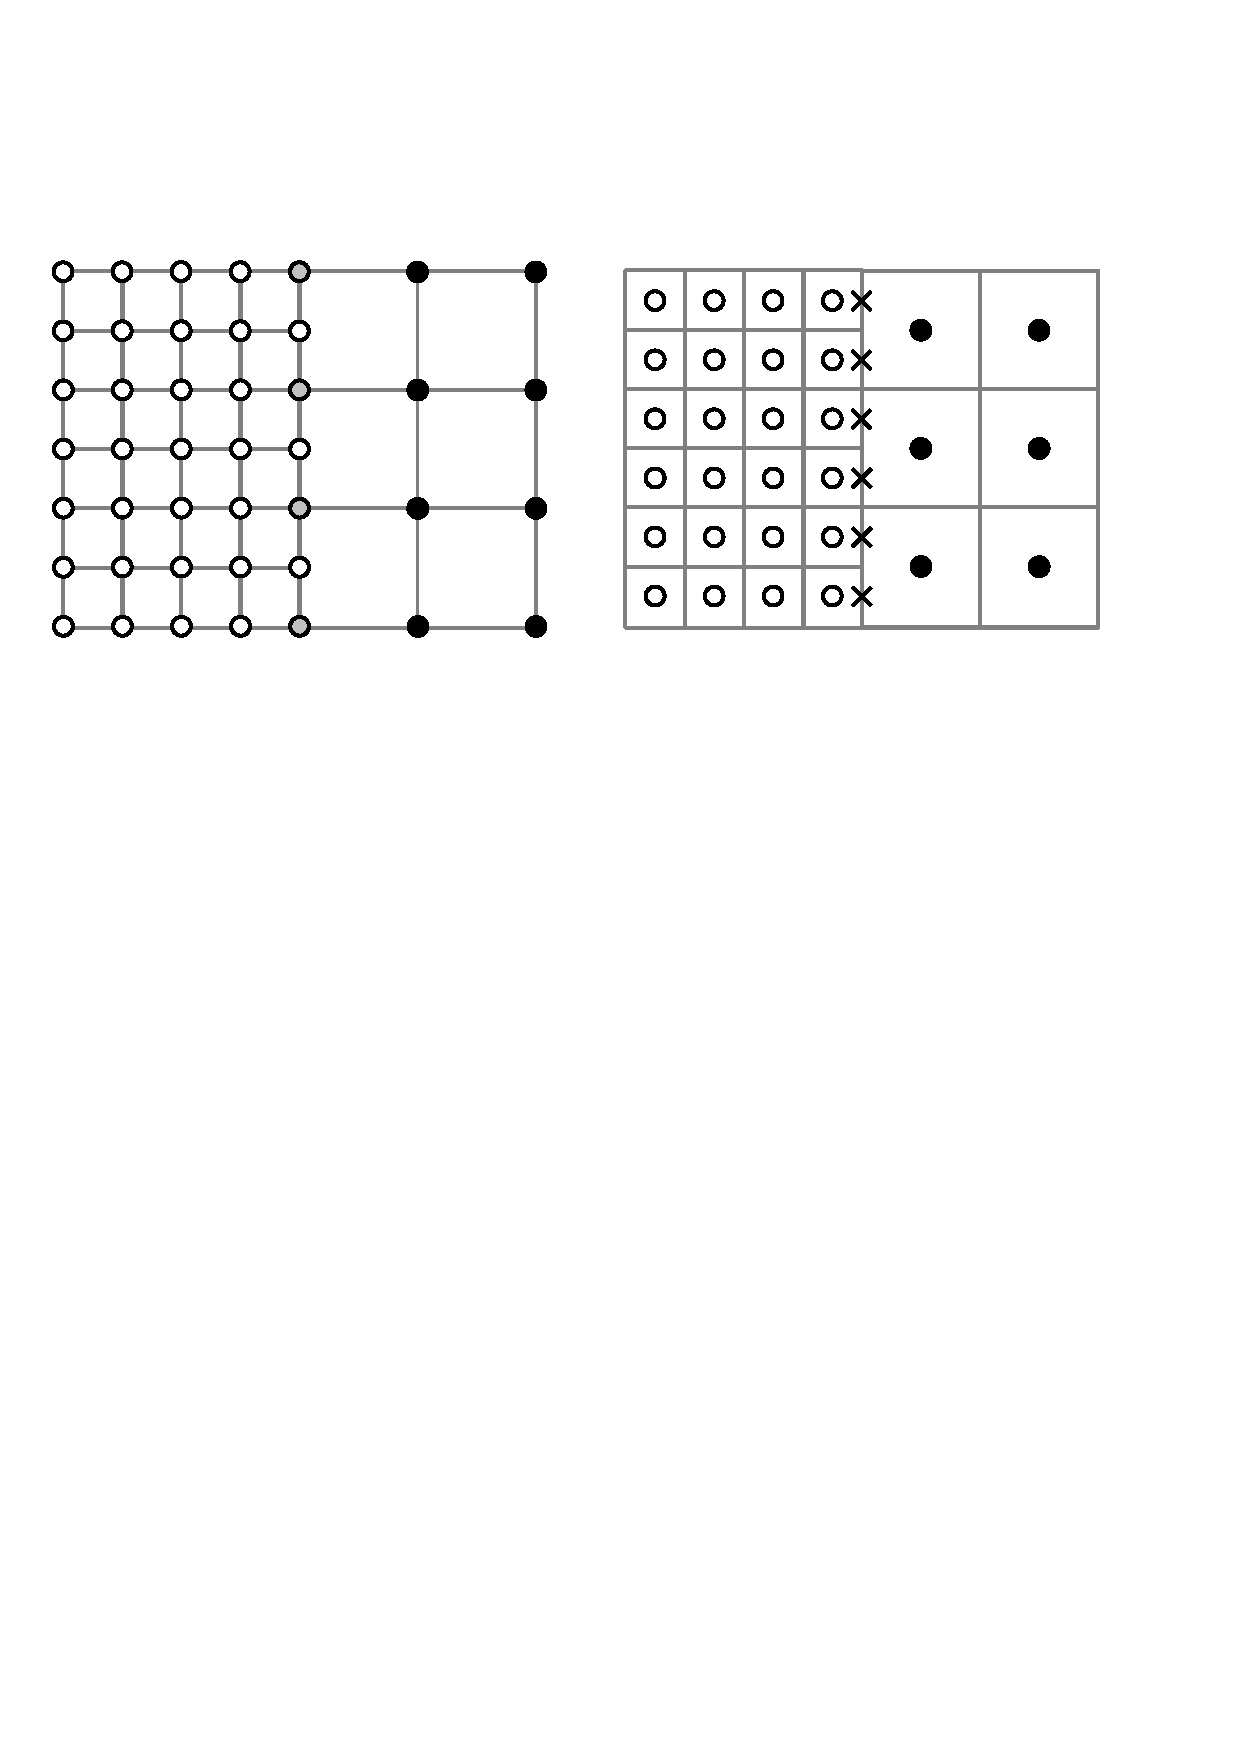
\includegraphics[width=100mm]{GridSolvers_hgMultigrid_f1}}
\end{center}
\caption{\label{Fig:GridSolvers_hgMultigrid_f1} Contrast between jumps of refinement in meshes used in the original paper
(left) and the oct-tree adapted method (right).}
\end{figure}

Another difference between the method of (Ricker 2008) and Huang \& Greengard is
that an oct-tree undoubtedly has neighboring blocks of the same
refinement, while a patch-based mesh would not. This problem is solved through
uniform prolongation of boundaries from coarse-to-fine, with simple relaxation
done to eliminate the slight error introduced between adjacent cells.

One final change between the two methods is that the original computes new
sources at the boundary between corrections, while the propagation here is done
through nested solves on various levels. 

The entire algorithm requires that the PARAMESH grid be reset such that all
blocks at refinement above some level $\ell$ are set as temporarily nonexistent.
This is required so that guardcell filling can occur at only that level,
neglecting blocks at a higher level of refinement.  This requires some global
communication by PARAMESH.

The method requires three basic operators over the solution $\phi$ on the grid:
taking the residual, restricting a fine-level function to coarser-level blocks,
and prolonging values from the coarse level to the faces of fine level blocks in
order to impose boundary values for the fine mesh problems.

The residual is calculated such that: 

\begin{equation}
\label{Eqn:residual}
R({\bf x}) \equiv  4\pi G \rho({\bf x}) - \nabla^2 \tilde\phi({\bf x})\ .
\end{equation}

This is accomplished through the application of the finite difference laplacian,
defined on level $\ell$ with length-scales $\Delta x_\ell$, $\Delta y_\ell$ and
$\Delta z_\ell$.

\begin{eqnarray}  % multiple lines needed in equation
{\cal D}_\ell\tilde\phi^{b\ell}_{ijk} & \equiv &
 {1\over\Delta x_\ell^2}\left(\tilde\phi^{b\ell}_{i+1,jk} -
                              2\tilde\phi^{b\ell}_{ijk} +
                              \tilde\phi^{b\ell}_{i-1,jk}\right)+ 
 {1\over\Delta y_\ell^2}\left(\tilde\phi^{b\ell}_{i,j+1,k} -
                              2\tilde\phi^{b\ell}_{ijk} +
                              \tilde\phi^{b\ell}_{i,j-1,k}\right)  \\
 & & + {1\over\Delta z_\ell^2}\left(\tilde\phi^{b\ell}_{ij,k+1} -
                              2\tilde\phi^{b\ell}_{ijk} +
                              \tilde\phi^{b\ell}_{ij,k-1}\right)\ .
\end{eqnarray}

The restriction operator ${\cal R}_\ell$ for block interior zones $(i,j,k)$ is:
\begin{equation}
({\cal R}_\ell\tilde\phi)^{{\cal P}(c),\ell}_{ijk} \equiv {1 \over {2^d}}
  \sum_{i'j'k'}
  \tilde\phi^{c,\ell+1}_{i'j'k'}\ ,
\end{equation}
where the indices $(i',j',k')$ refer to the zones in block $c$ that lie within
zone $(i,j,k)$ of block ${\cal P}(c)$.  We apply the restriction operator
throughout the interiors of blocks, but its opposite, the prolongation operator
${\cal I}_\ell$, need only be defined on the edges of blocks, because it is only
used to set boundary values for the direct single-block Poisson solver:
\begin{equation}
({\cal I}_\ell\tilde\phi)^{c,\ell+1}_{i'j'k'} \equiv \sum_{p,q,r = -2}^2
                 \alpha_{i'j'k'pqr}\tilde\phi^{{\cal P}(c),\ell}_{i+p,j+q,k+r}
\end{equation}
When needed, boundary zone values are set as for the difference operator.  We
use conservative quartic interpolation to set edge values, then solve with
homogeneous Dirichlet boundary conditions after using second-order
boundary-value elimination.  The coefficients $\alpha$ determine the
interpolation scheme. For the $-x$ face in 3D,
\begin{eqnarray}
\alpha_{1/2,j'k'pqr} &=& \beta_p \gamma_{j'q} \gamma_{k'r} \\
\nonumber
(\beta_p) &=& \left( -{1\over{12}}, {7\over{12}}, {7\over{12}},
                    -{1\over{12}}, 0 \right) \\
\nonumber
(\gamma_{j'q}) &=& \left\{\begin{array}{ll}\displaystyle
                   \left( -{3\over{128}}, {{11}\over{64}},
                                    1, -{{11}\over{64}}, {3\over{128}}\right)
                              & \ \ \ j' {\rm\ odd} \\
                   \displaystyle
                   \left( {3\over{128}}, -{{11}\over{64}},
                                    1, {{11}\over{64}}, -{3\over{128}}\right)
                              & \ \ \ j' {\rm\ even} 
                  \end{array} \right.
\end{eqnarray}
Interpolation coefficients are defined analogously for the other faces.
Note that we use half-integer zone indices to refer to averages over the
faces of a zone; integer zone indices refer to zone averages.

\subsubsection{The direct solver}
\label{Sec:direct solver}

In the case of problems with Dirichlet boundary conditions, a $d$-dimensional
fast sine transform is used.  The transform-space Green's Function for this is:

\begin{equation}
G^\ell_{ijk} = -16\pi G\left[ {1\over{\Delta x_\ell^2}}\sin^2\left({i\pi\over
2n_x}\right) + {1\over{\Delta y_\ell^2}}\sin^2\left({j\pi\over 2n_y}\right) +
{1\over{\Delta z_\ell^2}}\sin^2\left({k\pi\over 2n_z}\right)\right]^{-1}\ .
\end{equation} 

However, to be able to use the block solver in a general fashion, we must be
able to impose arbitrary boundary conditions per-block. In the case of
nonhomogenous Dirichlet boundary values, boundary value elimination may be used
to generalize the solver.  For instance, at the $-x$ boundary:

\begin{equation}
\label{Eqn:bvelim}
\rho_{1jk} \rightarrow \rho_{1jk} - {2\over\Delta x_\ell^2}\phi(x_{1/2},y_j,z_k)\ .
\end{equation}

For periodic problems only the coarsest block must be handled differently; block
adjacency for finer levels is handled naturally.  The periodic solver uses a
real-to-complex FFT with the Green's function:

\begin{equation}
G^\ell_{ijk} = \left\{\begin{array}{ll}\displaystyle {-16\pi G\left[
{1\over{\Delta x_\ell^2}}\sin^2\left({(i-1)\pi\over n_x}\right) + {1\over{\Delta
y_\ell^2}}\sin^2\left({(j-1)\pi\over n_y}\right) + {1\over{\Delta
z_\ell^2}}\sin^2\left({(k-1)\pi\over n_z}\right)\right]^{-1}}\\
\\
                               \hfill i, j, {\rm\ or\ } k \ne 1 \\
\\
\displaystyle
                   0\hfill i = j = k = 1 
                  \end{array} \right.
\end{equation}

This solve requires that the source be zero-averaged; otherwise the solution is
non-unique.  Therefore the source average is subtracted from all blocks.  In
order to decimate error across same-refinement-level boundaries, Gauss-Seidel
relaxations to the outer two layers of zones in each block are done after
applying the direct solver to all blocks on a level.  With all these components
outlined, the overall solve may be described by the following algorithm:

\begin{enumerate}
\item Restrict the source function $4\pi G\rho$ to all levels.  Subtract the
global average for the \code{periodic} case.
\item {\it Interpolation step:} For $\ell$ from 1 to $\ell_{\rm max}$,
      \begin{enumerate}
	\item Reset the grid so that $\ell$ is the maximum refinement level	
 	\item Solve ${\cal D}_\ell \tilde\phi^{b\ell}_{ijk} =
            4\pi G\rho^{b\ell}_{ijk}$ for all blocks $b$ on level $\ell$.
    	\item Compute the residual $R^{b\ell}_{ijk} = 4\pi G\rho^{b\ell}_{ijk} -
            {\cal D}_\ell \tilde\phi^{b\ell}_{ijk}$
    	\item For each block $b$ on level $\ell$ that has children, prolong
            face values for $\tilde\phi^{b\ell}_{ijk}$ onto each child block.
      \end{enumerate}
\item {\it Residual propagation step:} 
      Restrict the residual $R^{b\ell}_{ijk}$ to all levels.
\item {\it Correction step:} Compute the discrete $L_2$ norm of the residual over
      all leaf-node blocks and divide it by the discrete $L_2$ norm of the source
      over the same blocks. If the result is greater than a preset threshold
      value, proceed with a correction step: for each level $\ell$ from 1 to
      $\ell_{\rm max}$,
      \begin{enumerate}
	\item Reset the grid so that $\ell$ is the maximum refinement level
      	\item Solve ${\cal D}_\ell C^{b\ell}_{ijk} =
            R^{b\ell}_{ijk}$ for all blocks $b$ on level $\ell$.
      	\item Overwrite $R^{b\ell}_{ijk}$ with the new residual
            $R^{b\ell}_{ijk} - {\cal D}_\ell C^{b\ell}_{ijk}$ for all blocks
            $b$ on level $\ell$.
      \item Correct the solution on all leaf-node blocks $b$ on level $\ell$:
            $\tilde\phi^{b\ell}_{ijk} \rightarrow \tilde\phi^{b\ell}_{ijk} +
            C^{b\ell}_{ijk}$.
      \item For each block $b$ on level $\ell$ that has children, interpolate
            face boundary values of $C^{b\ell}_{ijk}$ for each child.
      \end{enumerate}
\item If a correction step was performed, return to the residual propagation
      step.
\end{enumerate}

The above procedure requires storage for $\tilde\phi$, $C$, $R$, and $\rho$ on
each block, for a total storage requirement of $4 n_x n_y n_z$ values per
block. Global communication is required in computing the tolerance-based
stopping criterion.


\subsubsection{A Hybrid Poisson Solver: Interfacing PFFT with Multigrid}
\label{PFFTMultigrid}
We can improve the performance of the Multigrid solver in Section
\ref{Sec:GridSolversMultigrid} by replacing single block FFTs with a
parallel FFT at a specified coarse level, where, the coarse level is
any level which is fully refined, i.e. containing blocks that
completely cover the computational domain.  Currently, we
automatically select the maximum refinement level that is fully
refined.

There is load imbalance in the Multigrid solver because each processor
performs single block FFTs on the blocks it owns.  At the coarse
levels there are relatively few blocks compared to available
processors which means many processors are effectively idle during the
coarse level solves.  The introduction of PFFT, and creation of a
hybrid solver, eliminates some of the coarse level solves.


The performance characteristics of the hybrid solver are described in
``Optimization of multigrid based elliptic solver for large scale
simulations in the Flash-X code'' (2012) which is available online at
\url{http://onlinelibrary.wiley.com/doi/10.1002/cpe.2821/pdf}.
Performance results are obtained using the PFFT\_PoissonFD unit test.



\subsection{Using the Poisson solvers}

The \code{GridSolvers} subunit solves the Poisson equation
(\eqref{Eqn:general Poisson}).
Two different elliptic solvers are supplied with Flash-X: a multipole
solver, suitable for approximately spherical source distributions,
and a multigrid solver, which can be used with general source distributions.
The multipole solver accepts only isolated boundary conditions, whereas
the multigrid solver supports Dirichlet, given-value, Neumann,
periodic, and isolated boundary conditions. Boundary conditions for the
Poisson solver are specified using an argument to the 
\api{Grid/Grid_solvePoisson}
routine which can be set from different runtime parameters depending on
the physical context in which the Poisson equation is being solved.
The \code{Grid_solvePoisson} routine is the primary entry point to the Poisson
solver module and has the following interface
\begin{quote}
\code{call Grid_solvePoisson (}{\it iSoln}\code{, }{\it iSrc}\code{, }
{\it bcTypes(6)}\code{, }{\it bcValues(2,6)}\code{, }{\it poisfact}\code{)}~,
\end{quote}
where {\it iSoln} and {\it iSrc} are the integer-valued
indices of the solution and source (density) variables,
respectively. {\it bcTypes(6)} is an integer array specifying the
type of boundary conditions to employ on each of the (up to) 6 sides
of the domain.  Index 1 corresponds to the -x side of the domain, 2 to
+x, 3 to -y, 4 to +y, 5 to -z, and 6 to +z.  The following values are
accepted in the array
\begin{center}
\begin{tabular}{cl}
{\it bcTypes} & Type of boundary condition\\
\hline
0 & Isolated boundaries\\
1 & Periodic boundaries\\
2 & Dirichlet boundaries\\
3 & Neumann boundaries\\
4 & Given-value boundaries\\
\hline
\end{tabular}
\end{center}
Not all boundary types are supported by all solvers.  In this release, {\it
bcValues(2,6)} is not used and can be filled arbitrarily.  Given-value
boundaries are treated as Dirichlet boundaries with the boundary values
subtracted from the outermost interior cells of the source; for this case the
solution variable should contain the boundary values in its first layer of
boundary cells on input to \code{Grid_solvePoisson}.  It should be noted that if
 \Paramesh is used, the values must be set for all levels.  Finally,
{\it poisfact} is real-valued and indicates the value of $\alpha$ multiplying the
source function in  (\eqref{Eqn:general Poisson}).


When solutions found using the Poisson solvers are to be differenced
(\eg, in computing the gravitational acceleration),
it is strongly recommended
that 
%% you use the \code{quadratic\_cartesian/cylindrical/spherical}
%% (quadratic) interpolants supplied  
%% by Flash-X. 
for AMR meshes, quadratic (or better) spatial
interpolation%\index{grid!interpolation}
at fine-coarse boundaries is chosen.  (For PARAMESH,
   this is automatically the case by default, and is handled correctly
   for Cartesian as well as the supported curvilinear geometries.
   But note that the default interpolation implementation may be changed 
   at configuration time with the 
   '\code{-gridinterpolation=}\ldots'%\index{setup!-gridinterpolation@\code{-gridinterpolation}}
   setup option;
   and with the default implementation, the interpolation order may be
   lowered with the \rpi{Grid/interpol_order} runtime parameter.)
If the order of the gridinterpolation of the mesh
is not of at least the same order as the differencing scheme used
in places like \api{physics/Gravity/Gravity_accelOneRow},
unphysical forces will be produced at refinement boundaries. Also, using
constant or linear grid interpolation may cause the multigrid solver to fail
to converge.


\subsubsection{Multipole (original version)}
\label{Sec:GridSolversMultipoleUsing}

The \code{poisson/multipole} sub-module takes two runtime parameters,
listed in \tblref{Tab:multipole parameters}.
Note that storage and CPU costs scale roughly as the square of
\code{mpole\_lmax}, so it is best to use this module only for nearly
spherical matter distributions.
\begin{table}
\caption{ Runtime parameters used with 
\code{poisson/multipole}.}
\label{Tab:multipole parameters} 
\begin{center}
\begin{tabular}{lllp{3in}}
Variable	& Type		& Default	& Description\\
\hline
\code{mpole\_lmax} & integer     & 10        & Maximum multipole moment\\
\code{quadrant}    & logical     & \code{.false.} & Use symmetry to solve a single
                                                  quadrant in 2D axisymmetric
                                                  cylindrical ($r,z$)
                                                  coordinates, instead of a
                                                  half domain.\\
\hline
\end{tabular}
\end{center}
\end{table}



\subsubsection{Multipole (improved version)}
\label{Sec:GridSolversMultipoleImprovedUsing}

To include the new multipole solver in a simulation, the best option
is to use the shortcut \code{+newMpole} at setup command line,
effectively replacing the following setup options :
\begin{codeseg}
-with-unit=Grid/GridSolvers/Multipole_new
-with-unit=physics/Gravity/GravityMain/Poisson/Multipole
-without-unit=Grid/GridSolvers/Multipole
\end{codeseg}
The improved multipole solver currently accepts only two setup parameters, either
one switching on multithreading:
\begin{itemize}
\item
{\bf threadBlockList}: enables multithreaded compilation and execution.
\item
{\bf threadWithinBlock}: enables multithreaded compilation and execution.
\end{itemize}
The names of these two setup parameters are missleading, since there is only one
universal threading strategy used. The use of these two setup parameters is a
temporary solution and will be replaced in near future by only one setup parameter.
\par
The improved multipole solver takes several runtime parameters,
whose functions are explained in detail below, together with comments about expected
time and memory scaling.

\begin{itemize}
\item
\rpi{Grid/mpole\_Lmax}: The maximum angular moment $L$ to be used for the multipole
Poisson solver. Depending on the domain geometry, the memory and time scaling factors
due to this variable alone are: i) 3D cartesian, 3D cylindrical $\rightarrow (L+1)(L+1)$, ii)
3D cartesian axisymmetric, 2D cylindrical, 2D spherical $\rightarrow (L+1)$,
iii) 1D spherical $\rightarrow 1$. Assuming no memory limitations, the multipole
solver is numerically stable for very large $L$ values. Runs up to $L=100$
for 3D cartesian domains have been performed. For 2D geometries, $L=1000$ was the
maximum tested.
\item
\rpi{Grid/mpole\_2DSymmetryPlane}: In 2D coordinates, this runtime parameter
enables the user to specify a plane of symmetry along the radial part of the
domain coordinates. In effect, this allows a reduction of the computational
domain size by one half. The code internally computes the multipole moments as if the
other symmetric part is present, i.e. no memory or execution time savings
can be achieved by this runtime parameter.
\item
\rpi{Grid/mpole\_3DAxisymmetry}: Forces rotational invariance around the main ($z$)
axis in 3D cartesian domains. The assumed rotational invariance in the $(x,y)$
plane effectively cancels all $m\neq 0$ multipole moments and one can restrict
the calculation to the $m=0$ multipole moments only. The time and memory
savings compared to a asymmetric 3D cartesian run is thus about a factor
of $(L+1)$. For 3D cylindrical domains, rotational invariance in the $(x,y)$
plane is equivalent of setting up the corresponding 2D cylindrical domain,
hence this runtime parameter is not honored for 3D cylindrical domains, and
the user is informed about the 3D to 2D cylindrical domain reduction possibility.
\item
\rpi{Grid/mpole\_DumpMoments}: This parameter is meant mainly for debugging purposes.
It prints the entire moment array for each radial bin for each time step.
This option should be used with care and for small problems only. The output
is printed to a text file named '$<$basenm$>$\_dumpMoments.txt', where $<basenm>$
is the base name given for the output files.
\item
\rpi{Grid/mpole\_PrintRadialInfo}: This parameter enables showing all detailed radial
bin information at each time step. This option is especially useful for optimizing
the radial bin sizes. The output is written to the text file '$<$basenm$>$\_printRadialInfo.txt'.
\item
\rpi{Grid/mpole\_IgnoreInnerZone}: Controls switching on/off the radial inner zone.
If it is set .true., the inner zone will not be recognized and all inner zone
radii will be treated statistically. This parameter is meant only for performing
some error analysis. For production runs it should always be at its default value
of false. Otherwise errors will be introduced in calculating the moments near
the expansion center.
\item
\rpi{Grid/mpole\_InnerZoneSize}: The size defining the discrete inner zone. The size
is given in terms of the inner zone smallest (atomic) radius, which is determined
at each time step by analyzing the domain grid structure around the multipolar origin
(expansion center). Only very rarely will this value ever have to be changed. The
default setting is very conservative and only under unusual circumstances
(ex: highly nonuniform grid around the expansion center) this might be necessary.
This value needs to be an integer, as it is used by the code to define dimensions
of certain arrays. Note, that by giving this runtime parameter a large integer
value (> 1000 for domain refinement levels up to 5) one can enforce the code to use
only non-statistical radial bins.
\item
\rpi{Grid/mpole\_InnerZoneResolution}: Defines the inner zone radial bin size for the
inner zone in terms of the inner zone smallest (atomic) radius.
Two inner zone radii will be considered different, if they are more than this
resolution value apart. A very tiny number (for example $10^{-8}$) will result in a complete
separation of all inner zone radii into separate radial bins. The default
value of $0.1$ should never be surpassed, and any attempt to do so will stop the
program with the appropriate information to the user. Likewise with a meaningless
resolution value of 0.
\item
\rpi{Grid/mpole\_MaxRadialZones}: The maximum number of outer radial zones to be used.
In contrast to the inner radial zone, the outer radial zones are much more important
for the user. Their layout defines the performance of the multipole solver both
in cpu time spent and accuracy of the potential obtained at each cell. The
default value of 1 outer radial zone at maximum refinement level leads to high
accuracy, but at the same time can consume quite a bit of memory, especially for full
3D runs. In these cases the user can specify several outer radial zones
each having their own radial bin size determination rule.
\item
\rpi{Grid/mpole\_ZoneRadiusFraction\_n}: The fraction of the maximum domain radius
defining the n-th outer zone maximum radial value. The total number of fractions given
must match the maximum number of outer radial zones specified and the fractions
must be in increasing order and less than unity as we move from the 1st outer zone
upwards. The last outer zone must always have a fraction of exactly 1. If not, the
code will enforce it.
\item
\rpi{Grid/mpole\_ZoneType\_n}: String value containing the outer radial zone type for
the n-th outer zone. If set to 'exponential', the radial equation $r(Q) = s \cdot \Delta r \cdot Q^t$,
defining the upper bound radius of the Q-th radial bin in the n-th outer zone,
is used. If set to 'logarithmic', the radial equation $r(Q) = s \cdot \Delta r \cdot (e^{Qt}-1)/(e^t-1)$ 
is used. In these equations $Q$ is a local radial bin counting index for each outer zone
and $s,t$ are parameters defining size and growth of the outer zone radial bins
(see below).
\item
\rpi{Grid/mpole\_ZoneScalar\_n}: The scalar value $s$ in the n-th outer radial zone equation
$r(Q) = s \cdot \Delta r \cdot Q^t$ or $r(Q) = s \cdot \Delta r \cdot (e^{Qt}-1)/(e^t-1)$. The
scalar is needed to be able to increase (or decrease) the size of the first radial
bin with respect to the default smallest outer zone radius $\Delta r$.
\item
\rpi{Grid/mpole\_ZoneExponent\_n}: The exponent value $t$ in the n-th outer radial zone
equations $r(Q) = s \cdot \Delta r \cdot Q^t$ or $r(Q) = s \cdot \Delta r \cdot (e^{Qt}-1)/(e^t-1)$.
The exponent controls the growth (shrinkage) in size of each radial bin with increasing bin index.
For the first equation, growing will occur for $t>1$, shrinking for $t<1$ and same size
for $t=1$. For the logarithmic equation, growing will occur for $t>0$, shrinking for
$t<0$, but the same size option $t=0$ will not work because the denominator becomes
undefined. The same size option must hence be treated using the exponential outer zone
type choice.
\item
{\bf Runtime parameter types, defaults and options}: 
\begin{center}
\begin{tabular}{llll}
Parameter & Type & Default & Options \\
\hline
\rpi{Grid/mpole\_Lmax}                      & integer & 0     & $>0$    \\
\rpi{Grid/mpole\_2DSymmetryPlane}           & logical & false & true    \\
\rpi{Grid/mpole\_3DAxisymmetry}             & logical & false & true    \\
\rpi{Grid/mpole\_DumpMoments}               & logical & false & true    \\
\rpi{Grid/mpole\_PrintRadialInfo}           & logical & false & true    \\
\rpi{Grid/mpole\_IgnoreInnerZone}           & logical & false & true    \\
\rpi{Grid/mpole\_InnerZoneSize}             & integer & 16    & $>0$    \\
\rpi{Grid/mpole\_InnerZoneResolution}       & real    & 0.1   & less than $0.1$ and $>0.0$ \\
\rpi{Grid/mpole\_MaxRadialZones}            & integer & 1     & $>1$    \\
\rpi{Grid/mpole\_ZoneRadiusFraction\_n}     & real    & 1.0   & less than $1.0$ and $>0.0$ \\
\rpi{Grid/mpole\_ZoneType\_n}               & string  & ''exponential''   & ''logarithmic'' \\
\rpi{Grid/mpole\_ZoneScalar\_n}             & real    & 1.0   & $>0.0$  \\
\rpi{Grid/mpole\_ZoneExponent\_n}           & real    & 1.0   & $>0.0$ (exponential) \\
                                 & real    &   -   & any $\neq 0$ (logarithmic)
\end{tabular}
\end{center}
\end{itemize}


\subsubsection{Tree Poisson solver}
\label{Sec:GridSolversBHTreeUsing}

The tree gravity solver can be included by \code{setup} or a \code{Config} file by
requesting

\bigskip

\texttt{physics/Gravity/GravityMain/Poisson/BHTree}

\bigskip

The current implementation works only in 3D Cartesian coordinates, and blocks
have to be logically cubic (\ie, \texttt{nxb}=\texttt{nyb}=\texttt{nzb}).
Physical dimensions of blocks can be arbitrary, however, some multipole
acceptance criteria can provide inaccurate error estimates with non-cubic
blocks. The computational domain can have arbitrary dimensions, and there can be
more blocks with \texttt{lrefine}=1 (\ie, \texttt{nblockx}, \texttt{nblocky} and
\texttt{nblockz} can have different values).

Runtime parameters \rpi{Grid/gr\_bhPhysMACTW} and \rpi{Grid/gr\_bhPhysMACComm}
control whether MACs of physical units are used in tree walk and communication,
respectively. If one of them (or both) is set \texttt{.false.}, only purely geometric
MAC is used for a corresponding part of the tree solver. It is not allowed to
set \rpi{Grid/gr\_bhPhysMACTW} = \texttt{.false.} and \rpi{Grid/gr\_bhPhysMACComm} =
\texttt{.true.}.

Runtime parameter \rpi{Grid/gr\_bhTreeLimAngle} allows to set the limit opening
angle for the purely geometrical MAC. Another condition controlling the
acceptance of the node for the calculations is that the {\em point-of-calculation}
must lie out of the box obtained by increasing the considered node by factor
\rpi{Grid/gr\_bhTreeSafeBox}.

Parameter \rpi{Grid/gr\_bhUseUnifiedTW} controls whether the Barnes-Hut like tree
walk algorithm is used (\texttt{.true.}) or whether an alternative algorithm is
used which checks the MAC only once for whole block for interactions with parent
blocks (\texttt{.false.}; see 8.10.2.4 for more details). The latter one is $10
- 20\%$ faster, however, it may lead to higher errors at block boundaries, in
particular if the gravity modules calculates the potential which is
subsequently differentiated to obtain gravitational acceleration. The tree walk
algorithm base on the priority queue is used if \code{grv\_bhMAC} is set to
\texttt{"SumSquare"}.

\bigskip

\begin{tabular}{|l|l|l|l|}
\hline
Variable & Type & Default & Description \\
\hline
\rpi{Grid/gr\_bhPhysMACTW}    & logical & .false. & whether physical MAC should be used in tree walk\\
\hline
\rpi{Grid/gr\_bhPhysMACComm}  &  logical & .false. & whether physical MAC should be used in communication\\
\hline
\rpi{Grid/gr\_bhTreeLimAngle} & real & $0.5$ & limiting opening angle\\
\hline
\rpi{Grid/gr\_bhTreeSafeBox}   & real & $1.2$ & relative size of restricted volume around node where the\\
                               &      &       & point-of-calculation is not allowed to be located\\
\hline
\rpi{Grid/gr\_bhUseUnifiedTW}   & logical  & .true.  & whether Barnes-Hut like tree walk algorithm should be used \\
\hline
\rpi{Grid/gr\_bhTWMaxQueueSize} & integer & .true.  & maximum length of the priority queue\\
\hline
\end{tabular}




\subsubsection{Multigrid}
\label{Sec:GridSolversMultigridUsing}

The \code{Grid/GridSolvers/Multigrid} module is appropriate for general source
distributions.  It solves Poisson's equation for 1, 2, and 3 dimensional
problems with Cartesian geometries.  It only supports the \Paramesh
Grid with one block at the coarsest level. For any other mesh
configuration it is advisable to use the hybrid solver, which switches
to a uniform grid exact solve when the specified level of coarsening
has been achieved. In most use cases for Flash-X, the multigrid solver
will be used to solve for Gravity (see: \secref{chp:Gravity}). It may
be included by \code{setup} or
\code{Config} by including:
\begin{codeseg}
physics/Gravity/GravityMain/Poisson/Multigrid
\end{codeseg}

The multigrid solver may also be included stand-alone using:
\begin{codeseg}
Grid/GridSolvers/Multigrid
\end{codeseg}

In which case the interface is as described above.  The supported boundary
conditions for the module are periodic, Dirichlet, given-value, and isolated.
Due to the nature of the FFT block solver, the same type of boundary condition
must be used in all directions.  Therefore, only the value of {\it bcTypes(1)}
will be considered in the call to \code{Grid_solvePoisson}.

The multigrid solver requires the use of two internally-used grid variables:
\code{isls} and \code{icor}.  These are used to store the calculated residual and solved-for
correction, respectively.  If it is used as a Gravity solver with isolated
boundary conditions, then two additional grid variables, \code{imgm} and
\code{imgp}, are used to store the image mass and image potential.  

\begin{center}
\begin{longtable}{lllp{2.25in}}

\caption{ \label{Tab:multigrid parameters} Runtime parameters used with
\code{Grid/GridSolvers/Multigrid}.} \\

Variable	& Type		& Default	& Description\\
\hline
\rpi{Grid/mg_MaxResidualNorm}
                & real          & $1\times 10^{-6}$  & Maximum ratio of the norm
                 of the residual to that of the right-hand side\\
\rpi{Grid/mg_maxCorrections}
                & integer & 100 & Maximum number of iterations to take\\
\rpi{Grid/mg_printNorm} & real & \code{.true.} & Print the norm ratio per-iteration\\
\rpi{Grid/mpole_lmax} & integer & 4 & The number of multipole moments used in the
isolated case\\
\hline

\end{longtable}
\end{center}

\subsubsection{Hybrid (Multigrid with PFFT)}
\label{Sec:GridSolversHybridUsing}

The hybrid solver can be used in place of the Multigrid solver for
problems with
\begin{itemize}
\item all-periodic
\item 2 periodic and 1 Neumann
\item 1 periodic and 2 Neumann
\end{itemize}
boundary conditions, if the default PFFT solver variant 
(called DirectSolver) is used.  
To use the hybrid solver in this way, add
\code{Grid/\-GridSolvers/\-Multigrid/\-PfftTopLevelSolve} to your
setup line or request the solver in your Simulation Config file (see
e.g. unitTest/PFFT\_PoissonFD).  The following setup lines create a
unit test that uses first the hybrid solver and then the standard
Multigrid solver

\begin{codeseg}
./setup unitTest/PFFT_PoissonFD -auto -3d -parfile=flash_pm_3d.par -maxblocks=800 +noio

./setup unitTest/PFFT_PoissonFD -auto -3d -parfile=flash_pm_3d.par -maxblocks=800 +noio
--without-unit=Grid/GridSolvers/Multigrid/PfftTopLevelSolve
--with-unit=Grid/GridSolvers/Multigrid
\end{codeseg}

It is also possible to select a different PFFT solver variant. In that case,
different combinations of boundary conditions for the Poisson problem may be
supported. 
The \code{HomBcTrigSolver} variant supports the largest set of
combinations of boundary conditions.
Use the \code{PfftSolver} setup variable to choose a variant.
Thus, appending \code{PfftSolver=HomBcTrigSolver} to the \code{setup}
chooses the \code{HomBcTrigSolver} variant.
When using the hybrid solver with the PFFT variants \code{HomBcTrigSolver} or
\code{SimplePeriodicSolver},
the runtime parameter \rpi{Grid/gr_pfftDiffOpDiscretize} should be set to 1.


The \code{Multigrid} runtime parameters given in the previous section also apply.


\subsection {HYPRE}
As a part of implicit time advancement we end up with a system of equations that needs to be solved at every time 
step. In \flashx the HYPRE linear algebra package is used to solve
these systems of equations. Therefore it is necessary to install Hypre
if this capability of Flash-X is to be used.\\

\api{Grid/Grid\_advanceDiffusion} is the API function which solves the system of equations. This API is provided by both
the split and unsplit solvers. The unsplit solver uses HYPRE to solve the system of equations and split solver does
a direct inverse using Thomas algorithm. Note that the split solver relies heavily on PFFT infrastructure
for data exchange and a significant portion of work in split \code{Grid\_advanceDiffusion} involves PFFT routines. In the 
unsplit solver the data exchange is implicitly done within HYPRE and is hidden. \\

The steps in unsplit \code{Grid\_advanceDiffusion} are as follows:
\begin{itemize}
\item {Setup HYPRE grid object}
\item {Exchange Factor B}
\item {Set initial guess}
\item {Compute HYPRE Matrix M such that B = MX}
\item {Compute RHS Vector B}
\item {Compute matrix A}
\item {Solve system AX = B}
\item {Update solution (in \flashx)} \\
\end{itemize} 

Mapping UG grid to HYPRE matrix is trivial, however mapping PARAMESH grid to a HYPRE matrix can be quite complicated. The 
process is simplified using the grid interfaces provided by HYPRE.
\begin{itemize}
\item {Struct Grid interface}
\item {SStruct Grid interface}
\item {IJ System interface}
\end{itemize} 

The choice of an interface is tightly coupled to the underlying grid on which the problem is being solved. We have chosen the SSTRUCT 
interface as it is the most compatible with the block structured AMR mesh in \flashx. Two terms commonly used in HYPRE terminology 
are part and box. We define these terms in equivalent \flashx terminology. A HYPRE box object maps directly to a leaf block in \flashx. 
The block is then defined by it's extents. In \flashx this information can be computed easily using a combination of \code{Grid\_getBlkCornerID} 
and \code{Grid\_getBlkIndexLimits}.All leaf blocks at a given refinement level form a HYPRE part. So number of parts in a typical 
\flashx grid would be give by,  \\

\code{nparts = leaf\_block(lrefine\_max) - leaf\_block(lrefine\_min) + 1} \\

So, if a grid is fully refined or UG, nparts = 1. However, there could still be more then one box object. \\

Setting up the HYPRE grid object is one of the most important step of the solution process. We use the SSTRUCT interface 
provided in HYPRE to setup the grid object. Since the HYPRE Grid object is mapped directly with \flashx grid, whenever the 
\flashx grid changes the HYPRE grid object needs to be updated. Consequentlywith AMR the HYPRE grid setup might happen multiple times. \\

Setting up a HYPRE grid object is a two step process, 
\begin{itemize}
\item Creating stenciled relationships.
\item Creating Graph relationships.
\end{itemize}

Stenciled relationships typically exist between leaf blocks at same refinement level (intra part) and graph relationships exist 
between leaf blocks at different refinement levels (inter part). The
fine-coarse boundary is handled in such a way that fluxes are
conserved at the interface (see \chpref{Chp:diffuse} for details). UG
does not require any graph relationships. \\

Whether a block needs a graph relationship depends on the refinement
level of it's neighbor. While this information is not directly
available in PARAMESH, it is possible to determine whether the block
neighbor is coarser or finer. Combining this information with the
constraint of at best a factor of two jump in refinement at block
boundaries, it is possible to compute the 
part number of a neighbor block, which in turn determines whether we need a graph. Creating a graph involves creating a link between all the cells on
the block boundary. \\

Once the grid object is created, the matrix and vector objects are
built on the grid object. The diffusion solve needs uninterpolated data from 
neighbor blocks even when there is a fine-coarse boundary, therefore
it cannot rely upon the guardcell fill process.
 A two step process is used to handle this situation, \\

\begin{itemize}
\item {Since HYPRE has access to X(at n, \ie, initial guess), the RHS vector B can be computed as MX where M is a modified Matrix.}
\item {Similarly the value of Factor B can be shared across the fine-coarse boundary by using \\
\code{Grid\_conserveFluxes},the fluxes need to be set in a intuitive to way to achieve the desired effect.} \\
\end{itemize}

With the computation of Vector B (RHS), the system can be solved using HYPRE and UNK can be updated. \\

\subsubsection{HYPRE Solvers}
\label{Sec:Hypre Solvers}
In \flashx  we use the HYPRE PARCSR storage format as this exposes the maximum number of iterative solvers. 

\begin{center}
\begin{longtable}{ll}
\caption{ \label{Tab:HYPRE solver types} Solvers, Preconditioners combinations used with \code{Grid/GridSolvers/HYPRE}.} \\
Solver        & Preconditioner  \\
\hline
PCG & AMG, ILU(0) \\
BICGSTAB & AMG, ILU(0) \\
GMRES & AMG, ILU(0) \\
AMG & - \\
SPLIT & - \\
\hline
\end{longtable}
\end{center}

{\bf Parallel runs:} One issue that has been observed is that there is a difference in the results produced by HYPRE using one or 
more processors. This would most likely be due to use of CG (krylov subspace methods), which involves an MPI\_SUM over the 
dot product of the residue. We have found this error to be dependent on the type of problem. One way to get across this problem is to use 
direct solvers in HYPRE like SPLIT. However we have noticed that direct solvers tend to be slow. THe released code has
an option to use the SPLIT solver, but this solver has not been extensively tested and was used only for internal debugging 
purposes and the usage of the HYPRE SPLIT solver in \flashx is purely experimental. \\ 

{\bf Customizing solvers:} HYPRE exposes a lot more parameters to tweak the solvers and preconditioners mentioned above. We have only used those 
which are applicable to general diffusion problems. Although in general these settings might be good enough it is by no means complete and 
might not be applicable to all class of  problems. Use of additional HYPRE parameters might require direct manipulation of \flashx code. \\

{\bf Symmetric Positive Definite (SPD) Matrix:}
PCG has been noticed to have convergence issues which might be related to (not necessarily),
\begin{itemize}
\item {A non-SPD matrix generated due to round of errors (only).} \\
\item {Use of BoomerAMG as PC (refer to HYPRE manual).} \\
\end{itemize}

The default settings use PCG as the solver with AMG as preconditioner. The following parameters 
can be tweaked at run time, \\

\begin{center}
\begin{longtable}{lllp{2.25in}}
\caption{ \label{Tab:HYPRE solver  parameters} Runtime parameters used with \code{Grid/GridSolvers/HYPRE}.} \\
Variable        & Type          & Default       & Description\\
\hline
\code{gr\_hyprePCType}
                & string          & \code{"hypre\_amg"}  & Algebraic Multigrid as Preconditioner \\
\code{gr\_hypreMaxIter}
                & integer & 10000 & Maximum number of iterations\\
\code{gr\_hypreRelTol} & real & $1\times 10^{-8}$ &  Maximum ratio of the norm
                 of the residual to that of the initial residue\\
\code{gr\_hypreSolverType} & string & \code{"hypre\_pcg"} & Type of linear solver, Preconditioned Conjugate gradient \\
\code{gr\_hyprePrintSolveInfo} & boolean & FALSE & enables/disables some basic solver information (for e.g number of iterations) \\
\code{gr\_hypreInfoLevel} & integer & 1 & Verbosity level of solver diagnostics (refer HYPRE manual). \\
\code{gr\_hypreFloor} & real & $1\times 10^{-12}$ & Used to floor the end solution. \\
\code{gr\_hypreUseFloor} & boolean & TRUE & whether to apply {gr\_hypreFloor} to floor results from HYPRE. \\
\hline
\end{longtable}
\end{center}




\section{Grid Geometry}
\label{Sec:Grid geometry}

Flash-X can use various kinds of coordinates (``\emterm{geometries}'')
for modeling physical problems. The available geometries
represent different (orthogonal) curvilinear coordinate systems.

The geometry for a particular problem is set at runtime
(after an appropriate invocation of \code{setup})
through
the \code{geometry} runtime parameter, which can take a value of
\code{"cartesian", "spherical", "cylindrical",} or \code{"polar"}. Together
with the dimensionality of the problem, this serves to completely
define the nature of the problem's coordinate axes
(\tblref{Tab:geometries}). Note that not all \unit{Grid} implementations
support all geometry/dimension combinations.
Physics units may also be limited in the geometries supported,
some may only work for Cartesian coordinates.

The core code of a \unit{Grid} implementation is not concerned with
the mapping of cell indices to physical coordinates; this is not required
for under-the-hood \unit{Grid} operations such as keeping track of which blocks
are neighbors of which other blocks, which cells need to be filled with data
from other blocks, and so on. Thus the physical domain can be logically modeled as
a rectangular mesh of cells, even in curvilinear coordinates.

There are, however, some areas where geometry needs to be taken into consideration.
The correct implementation of a given geometry%\index{mesh!geometry}%\index{geometry|see{mesh}}
requires that gradients and divergences have the appropriate area factors
and that the volume of a cell is computed properly for that geometry.
Initialization of the grid as well as AMR operations (such as restriction,
prolongation, and flux-averaging) must respect the geometry also.
Furthermore,
the hydrodynamic methods in Flash-X are finite-volume methods, so the
interpolation%\index{grid!interpolation}
must also be conservative in the given geometry.
The default mesh refinement criteria of \flashx also currently
take geometry into account, see \secref{Sec: refinement} above.

% %
\begin{table}[ht]

\caption{Different geometry types.
For each geometry/dimensionality combination,
the ``support'' column lists the \unit{Grid} implementations
that support it: pm4 stands for \Paramesh4.0 and \Paramesh4dev, pm2 for \Paramesh2, UG for
Uniform Grid implementations, respectively.
}
\label{Tab:geometries} 
\begin{center}
\begin{tabular}{lclcccc}
name       & dimensions & support  & axisymmetric & $X$-coord & $Y$-coord & $Z$-coord \\
\hline
cartesian   &    1       & pm4,pm2,UG & n            & $x$         &             &      \\
cartesian   &    2       & pm4,pm2,UG & n            & $x$         & $y$         &      \\
cartesian   &    3       & pm4,pm2,UG & n            & $x$         & $y$         & $z$  \\
\hline
cylindrical &    1       & pm4,UG   &   y            & $r$         &             &      \\
cylindrical &    2       & pm4,pm2,UG & y            & $r$         & $z$         &      \\
cylindrical &    3       & pm4,UG   &   n            & $r$         & $z$         & $\phi$ \\\hline
spherical   &    1       & pm4,pm2,UG & y            & $r$         &             &      \\
spherical   &    2       & pm4,pm2,UG & y            & $r$         & $\theta$    &      \\
spherical   &    3       & pm4,pm2,UG & n            & $r$         & $\theta$    & $\phi$ \\\hline
polar       &    1       & pm4,UG   &   y            & $r$         &             &      \\
polar       &    2       & pm4,pm2,UG & n            & $r$         & $\phi$      &      \\
\llap{}
\begin{minipage}{1.5in}
''polar + $z$''\\
(cylindrical with a different ordering of coordinates)
\end{minipage}
&  3       & ---      &   n            & $r$         & $\phi$      & $z$ \\
\hline
\end{tabular}
\end{center}

\end{table}
%

A \textbf{convention:}
in this section,
Small letters $x$, $y$, and $z$ are used with their usual meaning in
designating coordinate directions for specific coordinate systems:
\ie, $x$ and $y$ refer to directions in Cartesian coordinates,
and $z$ may refer to a (linear) direction in either Cartesian
or cylindrical coordinates.

On the other hand, capital symbols $X$, $Y$, and $Z$ are used to refer to the
(up to) three directions of any coordinate system, \ie,
the directions corresponding to the
\code{IAXIS}, \code{JAXIS}, and \code{KAXIS}
dimensions in \flashx, respectively.
Only in the Cartesian case do these correspond directly to
their small-letter counterparts. For other geometries,
the correspondence is given in \tblref{Tab:geometries}.



\subsection[Understanding 1D, 2D, Curvilinear]{Understanding 1D, 2D, and Curvilinear Coordinates}

In the context of Flash-X, curvilinear coordinates are most useful
with 1-d or 2-d simulations, and this is how they are commonly used.
But what does it mean to apply curvilinear coordinates in this way?
And what does it mean to do a 1D or a 2D simulation of threedimensional reality? 
Physical reality has three spatial
dimensions (as far as the physical problems simulated with Flash-X are concerned).
In Cartesian coordinates, it is relatively straightforward to understand
what a 2-d (or 1-d) simulation means: ``Just leave out one (or two) coordinates.''
This is less obvious for other coordinate systems, therefore
some fundamental discussion follows.

A reduced dimensionality (RD) simulation can be naively understood as
taking a cut (or, for 1-d, a linear probe) through the real 3-d problem.
However, there is also an assumption, not always explicitly stated, that
is implied in this kind of simulation: namely, that
the cut (or line) is representative of the 3-d problem.
This can be given a stricter  meaning:
it is assumed that the physics of the problem do not depend
on the omitted dimension (or dimensions).
A RD simulation can be a good description of a physical
system only to the degree that this assumption is warranted.
Depending on the nature of the simulated physical system,
non-dependence on the omitted dimensions may mean the absence
of force and/or momenta vector components in directions of
the omitted coordinate axes, zero net mass and energy flow
out of the plane spanned by the included coordinates, or similar.

For omitted dimensions that are lengths --- $z$ and possibly $y$ in Cartesian,
and $z$ in cylindrical and polar RD simulations ---
one may think of a 2-d cut as representing a (possibly very thin) layer
in 3-d space sandwiched between two parallel planes.
There is no \textit{a priori\/} definition of the thickness of the layer,
so it is not determined what 3-d volume should be asigned to a 2-d cell
in such coordinates. We can thus arbitrarily assign the length ``$1$''
to the edge length of a 3-d cell volume, making the volume equal
to the 2-d area.
We can understand generalizations of ``volume'' to 1-d, and of ``face
areas'' to 2-d and 1-d RD simulations with omitted linear coordinates,
in an equivalent way: just set the length of cell edges along omitted
dimensions to 1.


For omitted dimensions that are angles --- the $\theta$ and $\phi$ coordinates
on spherical, cylindrical, and polar geometries ---
it is easier to think of omitting an angle as the equivalent of integrating
over the full range of that angle coordinate (under the assumption that
all physical solution variables are independent of that angle).
Thus omitting an angle $\phi$ in these geometries implies
the assumption of axial symmetry, and this is noted in \tblref{Tab:geometries}.
Similarly, omitting both $\phi$ and $\theta$ in spherical coordinates
implies an assumption of complete spherical symmetry.
When $\phi$ is omitted, a 2-d cell actually represents the 3-d object
that is generated by rotating the 2-d area around a $z$-axis.
Similarly, when only $r$ is included, 1-d cells (\ie, $r$ intervals)
represent hollow spheres or cylinders.
(If the coordinate interval begins at $r_l=0.0$, the sphere or cylinder
is massive instead of hollow.)


As a result of these considerations,
the measures for cell (and block)
volumes and face areas in a simulation depends on the chosen geometry.
Formulas for the volume of a cell dependent on the geometry
are given in the geometry-specific sections further below.


As discussed in \secref{Sec:PARAMESH flux conservation},
to ensure conservation at a
jump in refinement in AMR grids, a flux correction step is taken.
The fluxes leaving the fine cells adjacent to a coarse cell are used
to determine more accurately the flux entering the coarse cell.
This step takes the coordinate geometry into account in order
to accurately determine the areas of the cell faces where
fine and coarse cells touch. By way of example,
an illustration is provided below in the
section on cylindrical geometry.

\subsubsection{Extensive Quantities in Reduced Dimensionality}\label{Sec:ExtQinRD}
The considerations above lead to some consequences for the understanding
of extensive quantities, like mass or energies, that may not be obvious.

The following discussion applies to geometries with
omitted dimensions that are lengths --- $z$ and possibly $y$ in Cartesian,
and $z$ in cylindrical and polar RD simulations.
We will consider Cartesian geometries as the most common case,
and just note that the remaining cases can be thought of analogously.

In 2D Cartesian, the ``volume'' of a cell should be $\Delta V = \Delta x\,\Delta y$.
We would like to preserve the form of equations that relate extensive quantities
to their densities, \eg,
$\Delta m = \rho \Delta V$ for mass and 
$\Delta E_{\mathrm tot} = \rho e_{\mathrm tot}\Delta V$ for total energy
in a cell. We also like to retain the usual definitions for
intensive quantities such as density $\rho$, including 
their physical values and units, so that material density $\rho$
is expressed in $g/cm^3$ (more generally $M/L^3$),
no matter whether 1D, 2D, or 3D.
We cannot satisfy both desiderata without modifying the interpretation
of ``mass'', ``energy'', and similar extensive quantities in the
system of equations modeled by Flash-X.

Specifically, in a 2D Cartesian simulation, we have to interpret ``mass''
as really representing a linear mass density, measured in $M/L$.
Similarly, an ``energy'' is really a linear energy density, \etc

In a 1D Cartesian simulation, we have to interpret ``mass''
as really representing a surface mass density, measured in $M/L^2$,
and an ``energy'' is really a surface energy density.

(There is a different point of view, which amounts to the same thing:
One can think of the ``mass'' of a cell (in 2D) as the physical mass contained in a
threedimensional cell of volume $\Delta x \Delta y \Delta z$ where the
cell height $\Delta z$
is set to be exactly 1 length unit. Always with the understanding that
``nothing happens'' in the $z$ direction.)

Note that this interpretation of ``mass'',``energy'', \etc
must be taken into account not just when examining the physics in individual cells,
but equally applies for quantities integrated over larger regions, including
the ``total mass'' or ``total energy'' \etc reported by Flash-X in \code{flash.dat}
files --- they are to be interpreted as (linear or surface) densities
of the nominal quantities (or, alternatively, as integrals over 1 length unit
in the missing Cartesian directions).

\subsection{Choosing a Geometry}

The user chooses a geometry by setting the
\rpi{Grid/geometry}
runtime parameter in \code{flash.par}. The default is
\code{"cartesian"} (unless overridden in a simulation's \code{Config} file).
Depending on the \unit{Grid} implementation used and the way it is
configured, the geometry may also have to be compiled into the program
executable and thus may have to be specified at configuration
time;
the \code{setup} flag 
\code{-geometry} %and/or \code{-curvilinear}
should be used for this purpose, see \secref{Sec:ListSetupArgs}.


The \rpi{Grid/geometry} runtime parameter is most useful
in cases where the geometry does not have to be specified
at compile-time, in particular for the Uniform Grid.
The runtime parameter will, however, always be considered
at run-time during \unit{Grid} initialization.
If the \rpi{Grid/geometry} runtime parameter is inconsistent
with a geometry specified at setup time,
Flash-X will then either
override the geometry specified at setup time (with a warning)
if that is possible, or it will abort.

This runtime parameter is used by the \unit{Grid} unit and
also by hydrodynamics solvers, which add the
necessary geometrical factors to the divergence terms.
Next we describe how user code can use the runtime parameter's value.

\subsection[Geometry Information in Code]{Getting Geometry Information in Program Code}
The \unit{Grid} unit provides an accessor
\api{Grid/Grid_getGeometry} property that returns
the geometry as an integer, which can be compared to the symbols
\{\code{CARTESIAN, SPHERICAL, CYLINDRICAL,
  POLAR}\}
% \index{mesh!geometry!CARTESIAN@\code{
%CARTESIAN}}%\index{mesh!geometry!SPHERICAL@\code{
%SPHERICAL}}%\index{mesh!geometry!CYLINDRICAL@\code{
%CYLINDRICAL}}%\index{mesh!geometry!POLAR@\code{POLAR}}
defined in \code{"constants.h"} to determine
which of the supported geometries we are using.  A unit writer can
therefore determine flow-control based on the geometry type (see
\figref{Code:geom_select}). Furthermore, this provides a mechanism
for a unit to determine at runtime whether it supports the current
geometry, and if not, to abort.

\begin{figure}[ht]
\begin{shrink}
\begin{fcodeseg}
  #include "constants.h"

  integer :: geometry

  call Grid_getGeometry(geometry)

  select case (geometry)

  case (CARTESIAN)

  ! do Cartesian stuff here ...

  case (SPHERICAL)

  ! do spherical stuff here ...

  case (CYLINDRICAL)

  ! do cylindrical stuff here ...

  case (POLAR)

  ! do polar stuff here ...

  end select
\end{fcodeseg}
\end{shrink}
\caption{\label{Code:geom_select} Branching based on geometry type}
\end{figure}

Coordinate information for the mesh can be determined via the
\api{Grid/Grid_getCellCoords} routine.
This routine can provide the coordinates of cells at the left
edge, right edge, or center.
The width of cells can be determined via the
\api{Grid/Grid_getDeltas} routine.
Angle values and differences are given in radians.
Coordinate information for a block of cells as a whole
is available through
\api{Grid/Grid_getBlkCenterCoords}
and
\api{Grid/Grid_getBlkPhysicalSize}.


The volume of a single cell can be obtained via the
\api{Grid/Grid_getSingleCellVol} or the
\api{Grid/Grid_getPointData}
routine.
Use the
\api{Grid/Grid_getBlkData},
\api{Grid/Grid_getPlaneData}, or
\api{Grid/Grid_getRowData}
routines with argument \code{dataType=CELL_VOLUME}
To retrieve cell volumes for more than one cell of a block.
To retrieve cell face areas, use the same \fcn{Grid\_get*Data}
interfaces with the appropriate \code{dataType} argument.

Note the following difference between the two groups of routines mentioned in
the previous two paragraphs: the routines for volumes and areas take
the chosen geometry into account in order to return geometric measures
of physical volumes and faces (or their RD equivalents).
On the other hand, the routines for coordinate values and widths
return values for $X$, $Y$, and $Z$ directly, without converting
angles to (arc) lengths.



\subsection{Available Geometries}

Currently, all of Flash-X's physics support one-, two-, and
(with a few exceptions explicitly stated in the appropriate chapters) three-dimensional
Cartesian grids.
Some units, including the Flash-X
\unit{Grid} unit and PPM hydrodynamics unit (\chpref{Chp:Hydrodynamics Unit}),
support additional geometries, such as two-dimensional cylindrical ($r,z$) grids,
one/two-dimensional spherical ($r$)/($r, \theta$) grids, and two-dimensional polar
($r, \phi$) grids. Some specific considerations for each geometry follow.

The following tables use the convention that
$r_l$ and $r_r$ stand for the values of the $r$ coordinate at the ``left'' and
``right'' end of the cell's $r$-coordinate range, respectively (\ie,
$r_l < r_r$ is always true), and $\Delta r = r_r-r_l$; and similar for
the other coordinates.

\subsubsection{Cartesian geometry}

Flash-X uses Cartesian (plane-parallel) geometry by default. This is
equivalent to specifying
\begin{codeseg}
   geometry = "cartesian"
\end{codeseg}
in the runtime parameter file.

% %%%It is not possible to define a volume for the 1- and 2-d Cartesian geometries,
% %%%so the length and area are returned respectively:

{\it Cell Volume in Cartesian Coordinates}
% \index{mesh!geometry!Cartesian}} 
\begin{minipage}{6in}
\renewcommand{\arraystretch}{1.5}
\begin{center}
\begin{tabular}{|l|c|}
\hline
1-d & $\Delta x$ \\
\hline
2-d & $\Delta x \Delta y$ \\
\hline
3-d & $\Delta x \Delta y \Delta z$  \\
\hline
\end{tabular}
\end{center}
\end{minipage}
%

% %%When running problems that have
% %%spherical or cylindrical symmetry on a Cartesian mesh, it is
% %%recommended that the refinement marking routine be designed to
% %%always refine the origin in order to minimize grid geometry effects
% %%there (see \secref{Sec:MarkRefLib}).

% %%The multigrid Poisson solver (\code{solvers/poisson/multigrid})
% %%supplied with Flash-X 2.5 works with Cartesian, 2D axisymmetric
% %%Cylindrical and 1/2D Spherical geometries. The multipole solver
% %%(\code{solvers/poisson/multipole}) works in any supported
% %%``closed'' geometry, including 1/2-D spherical, 2D axisymmetric
% %%cylindrical, and 3D Cartesian geometries.

\subsubsection{Cylindrical geometry}

%%Axisymmetric cylindrical geometry ($r,z$) is supported by Flash-X in
%%two dimensions (3D cylindrical ($r$,$z$,\/$\theta$) geometry is not
%%yet supported.)  It is assumed that the cylindrical radial
%%coordinate is in the $X$-direction, and the cylindrical
%%$z$-coordinate is in the $Y$-direction.
To run Flash-X with
cylindrical coordinates, the \code{geometry} parameter must be set
thus:

\begin{codeseg}
   geometry = "cylindrical"
\end{codeseg}


%%%1-d cylindrical is not supported.  In 2-d cylindrical
%%%coordinates, the domain is axisymmetric, so we integrate
%%%over the $\phi$ coordinate:

\vspace{1cm}

\begin{minipage}{6in}
\renewcommand{\arraystretch}{1.5}
\begin{center}
{\it Cell Volume in Cylindrical Coordinates}%\index{mesh!geometry!cylindrical} \\
\begin{tabular}{|l|c|}
\hline
1-d & $\pi (r_r^2 - r_l^2)$ \\
\hline
2-d & $\pi (r_r^2 - r_l^2) \Delta z$ \\
\hline
3-d & $\frac{1}{2} (r_r^2 - r_l^2) \Delta z \Delta \phi$ \\
\hline
\end{tabular}
\end{center}
\end{minipage}
%

As in other non-Cartesian
geometries, if the minimum radius is chosen to be zero
(\code{xmin = 0.}), the left-hand boundary type should be reflecting
(or \code{axisymmetric}).
Of all supported non-Cartesian geometries, the cylindrical is
in 2-d most similar to a 2-d coordinate system: it uses two
linear coordinate axes ($r$ and $z$) that form a rectangular
grid physically as well as logically.

As an illustrative example of the kinds of considerations
necessary in curved coordinates,
\figref{Fig:fluxes} shows a jump in refinement along the cylindrical
`$z$' direction.  When performing the flux correction step at a jump
in refinement, we must take into account the area of the annulus
through which each flux passes to do the proper weighting.  We
define the cross-sectional area through which the $z$-flux passes as
\begin{equation}
    A = \pi (r_r^2 - r_l^2)
\enskip .
\end{equation}
The flux entering the coarse cell above the
jump in refinement is corrected to agree with the fluxes leaving the
fine cells that border it.  This correction is weighted according to
the areas
\begin{equation}
   f_3 = \frac{A_1 f_1 + A_2 f_2}{A_3}~.
\end{equation}
%%
\begin{figure}
\begin{center}
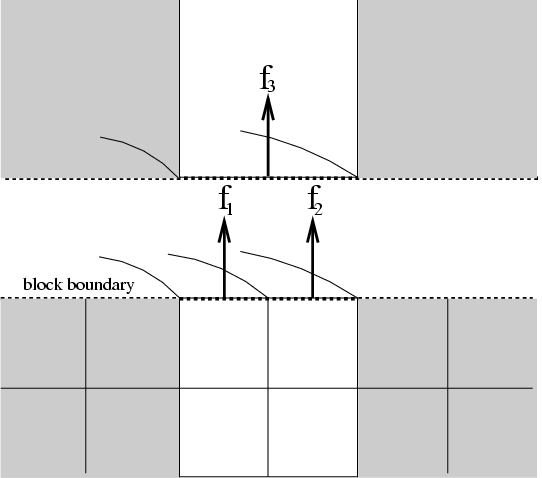
\includegraphics[height=2.5in]{Grid_flux2}
\end{center}
\caption{\label{Fig:fluxes} Diagram showing two fine cells and a
coarse cell at a jump in refinement in the cylindrical `$z$'
direction. The block boundary has been cut apart here for
illustrative purposes.  The fluxes out of the fine blocks are shown
as $f_1$ and $f_2$.  These will be used to compute a more accurate
flux entering the coarse flux $f_3$.  The area that the flux passes
through is shown as the annuli at the top of each fine cell and the
annulus below the coarse cell.}
\end{figure}

For fluxes in the radial direction, the cross-sectional area is independent
of the height, $z$, so the corrected flux is simply taken as the average of
the flux densities in the adjacent finer cells.

%%When using the multipole Poisson solver in 2D axisymmetric geometry,
%%the gravitational boundary type should be set to \code{"isolated"}.
%%In this geometry multipole moments $\ell > 0$ (\code{mpole\_lmax})
%%can now be accommodated, but only the $m=0$ terms are used.

\subsubsection{Spherical geometry}

One or two dimensional spherical problems can be performed by
specifying
\begin{codeseg}
   geometry = "spherical"
\end{codeseg}
in the runtime parameter file.


%%%In spherical coordinates, we can compute a true volume for all dimensions:


\vspace{1cm}
\begin{minipage}{6in}
\renewcommand{\arraystretch}{1.5}
\begin{center}
{\it Cell Volume in Spherical Coordinates}%\index{mesh!geometry!spherical} \\
\begin{tabular}{|l|c|}
\hline
1-d & $\frac{4}{3} \pi (r_r^3 - r_l^3)$ \\
\hline
2-d & $\frac{2}{3} \pi (r_r^3 - r_l^3) (\cos(\theta_l) - \cos(\theta_r))$ \\
\hline
3-d & $\frac{1}{3} (r_r^3 - r_l^3) (\cos(\theta_l) - \cos(\theta_r))
      \Delta \phi$ \\
\hline
\end{tabular}
\end{center}
\end{minipage}

\vspace{1cm}



%%Flux corrections use area weightings as for
%%2D cylindrical geometry.
If the minimum radius is chosen to be zero
(\code{xmin = 0.}), the left-hand boundary type should be reflecting.
%%When using the multipole Poisson solver spherical coordinates,
%%the gravitational boundary type should be \code{"isolated"}. Note that
%%in this case it does not make sense to use a multipole moment $\ell$
%%(\code{mpole\_lmax}) larger than 0.

\subsubsection{Polar geometry}
Polar geometry is a 2-D subset of 3-D cylindrical configuration
without the ``z'' coordinate. Such geometry is natural for studying
objects like accretion disks. This geometry can be selected by
specifying
\begin{codeseg}
   geometry = "polar"
\end{codeseg}
in the runtime parameter file.


%%In polar coordinates, the volumes are actually areas, since the domain is
%%always a disk:

\vspace{1cm}
\begin{minipage}{6in}
\renewcommand{\arraystretch}{1.5}
\begin{center}
{\it Cell Volume in Polar Coordinates}%\index{mesh!geometry!polar} \\
\begin{tabular}{|l|l|}
\hline
1-d & $ \pi (r_r^2 - r_l^2)$ \\
\hline
2-d & $ \frac{1}{2} (r_r^2 - r_l^2)\Delta \phi$ \\
\hline
3-d & $ \frac{1}{2} (r_r^2 - r_l^2)\Delta \phi \Delta z$ (not supported) \\
\hline
\end{tabular}
\end{center}
\end{minipage}
\vspace{1cm}

As in other non-Cartesian
geometries, if the minimum radius is chosen to be zero
(\code{xmin = 0.}), the left-hand boundary type should be reflecting.

%%Flux corrections use area weightings as
%%in other curvilinear coordinate systems.


%%Currently there is no support for self-gravity in polar geometry.


\subsection{Conservative Prolongation/Restriction on Non-Cartesian Grids}
\label{Sec:Non-Cart Prol/Rest}

When blocks are refined, we need to initialize the child data using the
information in the parent cell in a manner which preserves the
cell-averages in the coordinate system we are using.  When a block is
derefined, the parent block (which is now going to be a leaf block)
needs to be filled using the data in the child blocks (which are soon
to be destroyed).  The first procedure is called prolongation.%\index{grid!prolongation}
The latter is called restriction.%\index{grid!restriction}
Both of these procedures must respect
the geometry in order to remain conservative.  Prolongation and
restriction are also used when filling guard cells at jumps in
refinement.

\subsubsection{Prolongation}
When using a supported non-Cartesian geometry, Flash-X has to use
geometrically correct prolongation routines. These
are located in:
\begin{itemize}
\item {\code{source/Grid/GridMain/paramesh/Paramesh2/monotonic} (for
\Paramesh2)}
\item {\code{source/Grid/GridMain/paramesh/interpolation/Paramesh4/prolong}
(for \Paramesh4)}
\begin{comment}
\item {\code{source/Grid/GridMain/paramesh/Paramesh2/quadratic\_cylindrical} (for
cylindrical coordinates)}
\item {\code{source/Grid/GridMain/paramesh/Paramesh2/quadratic\_polar}
(for polar coordinates)}
\item {\code{source/Grid/GridMain/paramesh/Paramesh2/quadratic\_spherical}
(for spherical coordinates)}
\end{comment}
\end{itemize}
These paths will be be automatically added by the \code{setup} script when the
\code{-gridinterpolation=monotonic} option is in effect
%%(either explicitly or implicitly by specifying
%%a non-\code{cartesian} \code{-geometry}).
(which is the case by default, unless \code{-gridinterpolation=native} was specified).
The ``monotonic'' interpolation%\index{grid!interpolation}
scheme
used in both cases is taking geometry
into consideration and is appropriate for all supported geometries.

\begin{flashtip}
Some more specific \Paramesh2 interpolation schemes are included in the distribution
and might be useful for compatibility with \flashx:
\begin{itemize}
\item {\code{source/Grid/GridMain/paramesh/Paramesh2/quadratic\_cartesian}
(for Cartesian coordinates)}
\item {\code{source/Grid/GridMain/paramesh/Paramesh2/quadratic\_spherical}
(for spherical coordinates)}
\end{itemize}
Other geometry types and prolongation schemes can
be added in a manner analogous to the ones implemented here.

These routines could be included by specifying the correct path in your
\code{Units} file, or by using appropriate \code{-unit=} flags
for \code{setup}.
However, their use is not recommended.
\end{flashtip}


\subsubsection{Restriction}%\index{grid!restriction}
The default restriction routines understand the supported geometries
by default.  A cell-volume weighted average is used when restricting
the child data up to the parent.  For example, in 2-d, the restriction
would look like
\begin{equation}
\avgsub{f}{i,j} = \frac{V_{ic,jc} \avgsub{f}{ic,jc} +
                        V_{ic+1,jc} \avgsub{f}{ic+1,jc} +
                        V_{ic,jc+1} \avgsub{f}{ic,jc+1} +
                        V_{ic+1,jc+1} \avgsub{f}{ic+1,jc+1}}
                       {V_{i,j}}~,
\end{equation}
where $V_{i,j}$ is the volume of the cell with indices, $i, j$, and the
$ic, jc$ indices refer to the children.



\section{Unit Test}

The \unit{Grid} unit test has implementations to test  Uniform Grid
and \Paramesh. The Uniform Grid version of the test has two parts; the
latter portion is also tested in \Paramesh.
The test initializes the grid with a sinusoid function
\(\sin(x)\times\cos(y)\times\cos(z)\), distributed over a number of
processors. Knowing the configuration of processors, it is possible to
determine the part of the sinusoid on each processor. Since guardcells
are filled either from the interior points of the neighboring
processor, or from boundary conditions, it is also possible to predict
the values expected in guard cells on each processor. The first part of
the UG unit test makes sure that the actual received values of guard
cell match with the predicted ones. This process is carried out for
both cell-centered and face-centered variables.

The second part of the UG test, and the only part of the \Paramesh\ test,
exercises the get and put data functions. Since the \unit{Grid} unit
has direct access to all of its own data structures, it can compare
the values fetched using the getData functions against the directly
accessible values and report an error if they do not match.
The testing of the \unit{Grid} unit is not exhaustive, and given the complex
nature of the unit, it is difficult to devise tests that would do
so. However, the more frequently used functions are exercised in this test.


